%% (Master) Thesis template
% Template version used: v1.4
%
% Largely adapted from Adrian Nievergelt's template for the ADPS
% (lecture notes) project.


%% We use the memoir class because it offers a many easy to use features.
\documentclass[12pt,a4paper,titlepage]{memoir}

% no book layout now
\setulmarginsandblock{4cm}{4cm}{*}
\setlrmarginsandblock{4cm}{4cm}{*}

%% Packages
%% ========

\usepackage{xargs}                      % Use more than one optional parameter in a new commands
\usepackage[pdftex,dvipsnames]{xcolor}  % Coloured text etc.
% 
\usepackage[colorinlistoftodos,prependcaption,textsize=tiny]{todonotes}
\newcommandx{\unsure}[2][1=]{\todo[linecolor=red,backgroundcolor=red!25,bordercolor=red,#1]{#2}}
\newcommandx{\change}[2][1=]{\todo[linecolor=blue,backgroundcolor=blue!25,bordercolor=blue,#1]{#2}}
\newcommandx{\info}[2][1=]{\todo[linecolor=OliveGreen,backgroundcolor=OliveGreen!25,bordercolor=OliveGreen,#1]{#2}}
\newcommandx{\improvement}[2][1=]{\todo[linecolor=Plum,backgroundcolor=Plum!25,bordercolor=Plum,#1]{#2}}
\newcommandx{\thiswillnotshow}[2][1=]{\todo[disable,#1]{#2}}

%% LaTeX Font encoding -- DO NOT CHANGE
\usepackage[OT1]{fontenc}

%% Babel provides support for languages.  'english' uses British
%% English hyphenation and text snippets like "Figure" and
%% "Theorem". Use the option 'ngerman' if your document is in German.
%% Use 'american' for American English.  Note that if you change this,
%% the next LaTeX run may show spurious errors.  Simply run it again.
%% If they persist, remove the .aux file and try again.
\usepackage[ngerman]{babel}

%% Input encoding 'utf8'. In some cases you might need 'utf8x' for
%% extra symbols. Not all editors, especially on Windows, are UTF-8
%% capable, so you may want to use 'latin1' instead.
\usepackage[utf8]{inputenc}

%% This changes default fonts for both text and math mode to use Herman Zapfs
%% excellent Palatino font.  Do not change this.
\usepackage[sc]{mathpazo}
\usepackage[natbibapa]{apacite}

%% The AMS-LaTeX extensions for mathematical typesetting.  Do not
%% remove.
\usepackage{amsmath,amssymb,amsfonts,mathrsfs}

%% NTheorem is a reimplementation of the AMS Theorem package. This
%% will allow us to typeset theorems like examples, proofs and
%% similar.  Do not remove.
%% NOTE: Must be loaded AFTER amsmath, or the \qed placement will
%% break
\usepackage[amsmath,thmmarks]{ntheorem}

%% LaTeX' own graphics handling
\usepackage{graphicx}
\usepackage{lscape}

\addto\extrasngerman{\def\figureautorefname{Abbildung}}
\addto\extrasngerman{\def\sectionautorefname{Abschnitt}}
\addto\extrasngerman{\def\subsectionautorefname{Unterabschnitt}}

\graphicspath{ {bilder/} }

%% We unfortunately need this for the Rules chapter.  Remove it
%% afterwards; or at least NEVER use its underlining features.
\usepackage{soul}

%% This allows you to add .pdf files. It is used to add the
%% declaration of originality.
\usepackage{pdfpages}

%% Some more packages that you may want to use.  Have a look at the
%% file, and consult the package docs for each.
%% See the TeXed file for more explanations

%% [OPT] Multi-rowed cells in tabulars
%\usepackage{multirow}

%% [REC] Intelligent cross reference package. This allows for nice
%% combined references that include the reference and a hint to where
%% to look for it.
\usepackage{varioref}

%% [OPT] Easily changeable quotes with \enquote{Text}
%\usepackage[german=swiss]{csquotes}

%% [REC] Format dates and time depending on locale
\usepackage{datetime}

%% [OPT] Provides a \cancel{} command to stroke through mathematics.
%\usepackage{cancel}

%% [NEED] This allows for additional typesetting tools in mathmode.
%% See its excellent documentation.
\usepackage{mathtools}

%% [ADV] Conditional commands
%\usepackage{ifthen}

%% [OPT] Manual large braces or other delimiters.
%\usepackage{bigdelim, bigstrut}

%% [REC] Alternate vector arrows. Use the command \vv{} to get scaled
%% vector arrows.
\usepackage[h]{esvect}

%% [NEED] Some extensions to tabulars and array environments.
\usepackage{array}

%% [OPT] Postscript support via pstricks graphics package. Very
%% diverse applications.
%\usepackage{pstricks,pst-all}

%% [?] This seems to allow us to define some additional counters.
%\usepackage{etex}

%% [ADV] XY-Pic to typeset some matrix-style graphics
%\usepackage[all]{xy}

%% [OPT] This is needed to generate an index at the end of the
%% document.
%\usepackage{makeidx}

%% [OPT] Fancy package for source code listings.  The template text
%% needs it for some LaTeX snippets; remove/adapt the \lstset when you
%% remove the template content.
\usepackage{listings}
\lstset{language=TeX,basicstyle={\normalfont\ttfamily}}
%% [REC] Fancy character protrusion.  Must be loaded after all fonts.
\usepackage[activate]{pdfcprot}

%% [REC] Nicer tables.  Read the excellent documentation.
\usepackage{booktabs}


%% Our layout configuration.  DO NOT CHANGE.
%% Memoir layout setup

%% NOTE: You are strongly advised not to change any of them unless you
%% know what you are doing.  These settings strongly interact in the
%% final look of the document.

% Dependencies
\usepackage{HSLUlogo}

% Turn extra space before chapter headings off.
\setlength{\beforechapskip}{0pt}

\nonzeroparskip
\parindent=0pt
\defaultlists

% Chapter style redefinition
\makeatletter

\if@twoside
  \pagestyle{Ruled}
  \copypagestyle{chapter}{Ruled}
\else
  \pagestyle{ruled}
  \copypagestyle{chapter}{ruled}
\fi
\makeoddhead{chapter}{}{}{}
\makeevenhead{chapter}{}{}{}
\makeheadrule{chapter}{\textwidth}{0pt}
\copypagestyle{abstract}{empty}

\makechapterstyle{bianchimod}{%
  \chapterstyle{default}
  \renewcommand*{\chapnamefont}{\normalfont\Large\sffamily}
  \renewcommand*{\chapnumfont}{\normalfont\Large\sffamily}
  \renewcommand*{\printchaptername}{%
    \chapnamefont\centering\@chapapp}
  \renewcommand*{\printchapternum}{\chapnumfont {\thechapter}}
  \renewcommand*{\chaptitlefont}{\normalfont\huge\sffamily}
  \renewcommand*{\printchaptertitle}[1]{%
    \hrule\vskip\onelineskip \centering \chaptitlefont\textbf{\vphantom{gyM}##1}\par}
  \renewcommand*{\afterchaptertitle}{\vskip\onelineskip \hrule\vskip
    \afterchapskip}
  \renewcommand*{\printchapternonum}{%
    \vphantom{\chapnumfont {9}}\afterchapternum}}

% Use the newly defined style
\chapterstyle{bianchimod}

\setsecheadstyle{\Large\bfseries\sffamily}
\setsubsecheadstyle{\large\bfseries\sffamily}
\setsubsubsecheadstyle{\bfseries\sffamily}
\setparaheadstyle{\normalsize\bfseries\sffamily}
\setsubparaheadstyle{\normalsize\itshape\sffamily}
\setsubparaindent{0pt}

% Set captions to a more separated style for clearness
\captionnamefont{\sffamily\bfseries\footnotesize}
\captiontitlefont{\sffamily\footnotesize}
\setlength{\intextsep}{16pt}
\setlength{\belowcaptionskip}{1pt}

% Set section and TOC numbering depth to subsection
\setsecnumdepth{subsection}
\settocdepth{subsection}

%% Titlepage adjustments
\pretitle{\vspace{0pt plus 0.7fill}\begin{center}\HUGE\sffamily\bfseries}
\posttitle{\end{center}\par}
\preauthor{\par\begin{center}\let\and\\\Large\sffamily}
\postauthor{\end{center}}
\predate{\par\begin{center}\Large\sffamily}
\postdate{\end{center}}

\def\@advisors{}
\newcommand{\advisors}[1]{\def\@advisors{#1}}
\def\@department{}
\newcommand{\department}[1]{\def\@department{#1}}
\def\@thesistype{}
\newcommand{\thesistype}[1]{\def\@thesistype{#1}}

\renewcommand{\maketitlehooka}{\noindent\HSLUlogo[2in]}

\renewcommand{\maketitlehookb}{\vspace{1in}%
  \par\begin{center}\Large\sffamily\@thesistype\end{center}}

\renewcommand{\maketitlehookd}{%
  \vfill\par
  \begin{flushright}
    \sffamily
    \@advisors\par
    \@department, Hochschule Luzern
  \end{flushright}
}

\checkandfixthelayout

\setlength{\droptitle}{-48pt}

\makeatother

% This defines how theorems should look. Best leave as is.
\theoremstyle{plain}
\setlength\theorempostskipamount{0pt}

%%% Local Variables:
%%% mode: latex
%%% TeX-master: "thesis"
%%% End:


%% Theorem environments.  You will have to adapt this for a German
%% thesis.
%% Theorem-like environments

%% This can be changed according to language. You can comment out the ones you
%% don't need.

\numberwithin{equation}{chapter}

%% German theorems
%\newtheorem{satz}{Satz}[chapter]
%\newtheorem{beispiel}[satz]{Beispiel}
%\newtheorem{bemerkung}[satz]{Bemerkung}
%\newtheorem{korrolar}[satz]{Korrolar}
%\newtheorem{definition}[satz]{Definition}
%\newtheorem{lemma}[satz]{Lemma}
%\newtheorem{proposition}[satz]{Proposition}

%% English variants
\newtheorem{theorem}{Theorem}[chapter]
\newtheorem{example}[theorem]{Example}
\newtheorem{remark}[theorem]{Remark}
\newtheorem{corollary}[theorem]{Corollary}
\newtheorem{definition}[theorem]{Definition}
\newtheorem{lemma}[theorem]{Lemma}
\newtheorem{proposition}[theorem]{Proposition}

%% Proof environment with a small square as a "qed" symbol
\theoremstyle{nonumberplain}
\theorembodyfont{\normalfont}
\theoremsymbol{\ensuremath{\square}}
\newtheorem{proof}{Proof}
%\newtheorem{beweis}{Beweis}


%% Helpful macros.
%% Custom commands
%% ===============

%% Special characters for number sets, e.g. real or complex numbers.
\newcommand{\C}{\mathbb{C}}
\newcommand{\K}{\mathbb{K}}
\newcommand{\N}{\mathbb{N}}
\newcommand{\Q}{\mathbb{Q}}
\newcommand{\R}{\mathbb{R}}
\newcommand{\Z}{\mathbb{Z}}
\newcommand{\X}{\mathbb{X}}

%% Fixed/scaling delimiter examples (see mathtools documentation)
\DeclarePairedDelimiter\abs{\lvert}{\rvert}
\DeclarePairedDelimiter\norm{\lVert}{\rVert}

%% Use the alternative epsilon per default and define the old one as \oldepsilon
\let\oldepsilon\epsilon
\renewcommand{\epsilon}{\ensuremath\varepsilon}

%% Also set the alternate phi as default.
\let\oldphi\phi
\renewcommand{\phi}{\ensuremath{\varphi}}


%% Make document internal hyperlinks wherever possible. (TOC, references)
%% This MUST be loaded after varioref, which is loaded in 'extrapackages'
%% above.  We just load it last to be safe.
\usepackage[linkcolor=black,colorlinks=true,citecolor=black,filecolor=black]{hyperref}


%% longtable
\usepackage{longtable}

%% sourcecode
\usepackage{minted}

\providecommand*{\listingautorefname}{Listing}


%% Document information
%% ====================

\title{Prototyping einer webbasierten Visualisierung zur intuitiven Interaktion mit einem Wissensnetzwerk}
\author{Andreas Waldis, Patrick Siegfried}
\thesistype{}
\advisors{Advisor: Dr.\ Michael Kaufmann}
\department{Departement Informatik}
\date{\today}

\begin{document}

\listoftodos

\frontmatter


%% Title page is autogenerated from document information above.  DO
%% NOT CHANGE.
\begin{titlingpage}
  \calccentering{\unitlength}
  \begin{adjustwidth*}{\unitlength-24pt}{-\unitlength-24pt}
    \maketitle
  \end{adjustwidth*}
\end{titlingpage}

%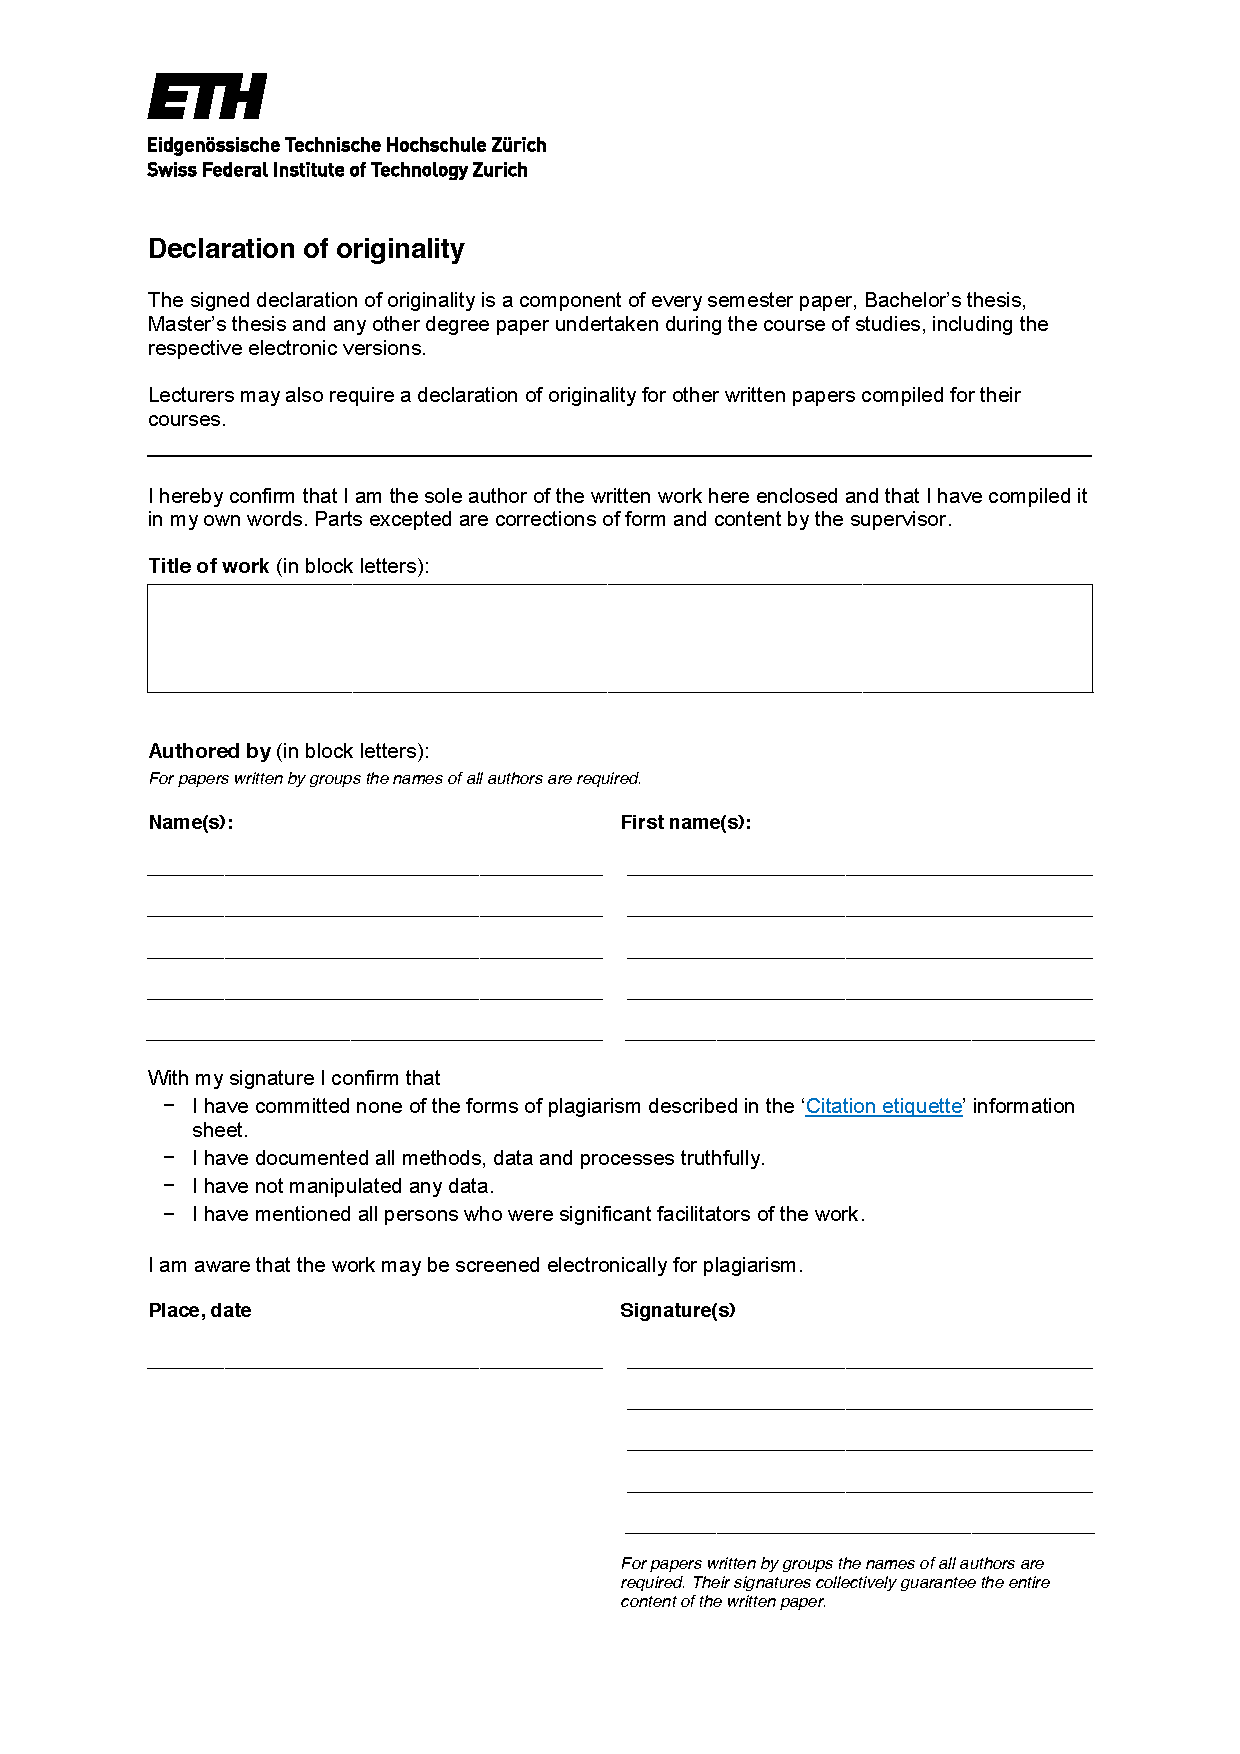
\includepdf[pages={-}]{declaration-originality.pdf}

%% The abstract of your thesis.  Edit the file as needed.
%\begin{abstract}
  Im Rahmen des Informatikprojekts wurde ein Prototyp für die Visualisierung und Interaktion von \gls{Netzwerk}[en] erarbeitet. Dazu wurden mithilfe der Spezifikation von funktionalen Anforderungen verschiedene \gls{Framework}[s] für die Grundlage der Entwicklung evaluiert. Anschliessend wurde die für den Anwendungsfall beste Wahl getroffen.
  
  Der Prototyp bietet eine Benutzeroberfläche, welche sowohl auf kleinen und grossen Bildschirmen, mit Touch-Gesten oder der Maus und der Tastatur, verwendet werden kann.
  Der resultierende Prototyp wurde als selbständiges Software-Paket entwickelt. Dadurch kann dieser in beliebigen Applikationen verwendet werden. In der letzten Projektphase wurde der Prototyp schlussendlich in den bestehenden \gls{ikc-core} integriert.
\end{abstract}


%% TOC with the proper setup, do not change.
\cleartorecto
\setcounter{tocdepth}{3}
\tableofcontents
\mainmatter

%% Your real content!
\chapter{Einleitung}

Im Hasler-Projekt Intuitive Knowledge Connectivity (IKC) wird ein Prototyp für plattformübergreifendes Wissensnetzwerk erstellt. Die grundlegende Datenbank basiert auf einen Netzwerk (einem gerichteten beschrifteten Property-Graph), hat aber bisher nur eine technische Konsole. Eine ideale grafische Benutzerschnittstelle stellt das Netzwerk oder Teilausschnitte daraus visuell und zweidimensional dar, und stellt beschriftete Knoten und Pfeile grafisch dar. Dies ermöglicht eine einfache und übersichtliche Repräsentation und eine intuitive Interaktion mit den gegebenen Kanten und Knoten. Der bestehende Prototyp implementiert die grundlegenden Datenbankoperationen (CRUD) und die Verknüpfung von Knoten mit Drag and Drop. Auf dieser Kern-Software soll aufgebaut werden, um diese hinsichtlich intuitiver Benutzung zu erweitern, damit mit mehreren Knoten im Netzwerk gleichzeitig und visuell gearbeitet werden kann. Dies soll in erster Linie auf dem Touchscreen (mobil / Tablet) und in zweiter Linie responsive mit dem gleichen Code auch mit Bildschirm, Tastatur und Maus / Touchpad bedienbar sein.

\chapter{Projektmanagement}

Führung und Kontrolle des Projekts werden im folgenden Kapitel aufgezeigt. Das Projektmanagement funktioniert agil, dafür werden geeignete Hilfsmittel eingesetzt. 

\section{Ausgangslage}
Aus dem Forschungsprojekt \textit{Intuitive Knowledge Connectivity} \cite{ikc:hslu} ging neben einer Publikation \cite{ikc-paper:hslu} auch ein Software-Prototyp (\textit{ikc-core}) hervor. Das Projekt beschäftigt sich mit einem intuitiven Umgang mit Daten aus diversen Cloud-Dienstleistern, beispielsweise \textit{Dropbox}, \textit{Evernote} und vielen mehr. Diese werden, ebenfalls \textit{cloudbasiert}, gespeichert und verteilt. Der Mehrwert entsteht durch Verknüpfung der verschiedenen Daten zu einem gesamtheitlichen Ganzen. Diese Verknüpfungen sind be\-nutzer\-bas\-iert und werden mithilfe einer Graph-Datenbank gehandhabt.

Da beide Projektarbeiter ebenfalls am Forschungsprojekt tätig sind, ist das Grundlagewissen bereits grösstenteils vorhanden. Die Arbeit am Forschungsprojekt und am PAWI verlaufen parallel weiter. Um eine adäquate Trennung der beiden Projekte zu gewährleisten, wird im \autoref{sec:scope} näher auf die Gegebenheiten eingegangen.

\subsection{Internationale Projektorganisation}
\label{subsec:international}
Da mit Andreas Waldis ein Team-Mitglied während des Projekts in den Vereinigten Staaten im Austauschsemester weilt, müssen einige zusätzliche organisatorische Massnahmen ergriffen werden. Diese umfassen die folgenden Tools und Arbeitsweisen:
\begin{itemize}
\item Zeitverschiebung: Zwischen den beiden Zeitzonen von Luzern (\textit{UTC+01:00}) und West Lafayette (\textit{UTC-05:00}) beträgt sechs Stunden. Daher werden Sitzungen überwiegend Nachmittags nach 14:00 angesetzt. 
\item Projektplanung: Die Projektdauer wurde für diesen speziellen Fall um 6 Wochen auf Ende Januar erweitert. Dies ermöglicht den verschiedenen Teammitglieder entsprechend ihrer Auslastung zu arbeiten. Insbesondere für Andreas Waldis, welcher bereits im Dezember die Abschlussprüfungen hat. 
\item Werkzeuge: Es werden verschiedene zusätzliche Werkzeuge verwendet, um eine möglichst optimale Kommunikation und Kollaboration zu gewährleisten. Dazu gehören:
\begin{enumerate}
\item Slack: Ein Messenger, welcher für die Verwendung im professionellen Umfeld ausgelegt ist. So können beispielsweise verschiedene Cloud-Services integriert werden.\cite{SlackBel4:online}
\item Skype \& Discord \cite{DiscordF75:online}\cite{SkypeKos72:online}: Beides Werkzeuge für Video- und Audio-Sitzungen. Skype ist wohlbekannt. Discord hingegegen ist spezialisiert für Gamer und beinhaltet ein umfangreicheres Chat-System.
\item Targetprocess \cite{targetprocess}: Vergleichbar mit dem bekannten ScrumDo \cite{scrumdo}. Im Gegensatz dazu verfügt Targetprocess über eine moderne Benutzeroberfläche und scheint für den Verwendungszweck im Allgemeinen idealer zu sein.
\item Sharelatex \cite{sharelatex}: Online Kollaborationstools für Latex. Anstelle von lokalen Installationen in einem gemeinsamen Versionverwaltungssystem, wird einfach direkt online am selben Dokument gearbeitet.
\item draw.io\cite{draw:io}: Werkzeug um online Diagramme zu zeichnen. Diese können ebenfalls gemeinsam und gleichzeitig gezeichnet werden. Es wird aber vor allem darum verwendet, weil es einfach und schnell möglich ist alles Mögliche zu zeichnen.
\end{enumerate}
\end{itemize}

\section{Scope}
\label{sec:scope}

Die Schwierigkeit in der Abgrenzung liegt zu einem grossen Teil im parallel laufenden Projekt \textit{IKC}. Der bestehende \textit{ikc-core} wird soweit vorbereitet, dass die Visualisierung ohne Zusatzaufwand integriert werden kann. Darunter gehören Arbeiten betreffend Schnittstellen, absenden von allfälligen Event und dergleichen. Die genaue Spezifikation ist im Lösungskonzept noch zu erarbeiten.

Weiter ist zu betonen, dass die intuitive Bedienung (\textit{Usability} und auch \textit{User Experience}) nach bestem Wissen und Gewissen angestrebt wird. Allerdings handelt es sich bei den Projektmitarbeitern um Informatiker ohne grundlegenden Kenntnisse in den angesprochenen Bereichen. Daher wird das Resultat eine objektive Sicht auf die Oberfläche sein, optimiert zusammen mit dem Projektpartner.

\section{Projektstrukturplan}
Die \autoref{fig:projektstrukturplan} gewährt einen Überblick über das Projekt. Sie stellt die wichtigsten Bereiche und Phasen dar, worin die Arbeit grob eingegliedert werden kann:
\begin{enumerate}
    \item Die \textbf{Projektführung} beinhaltet die Planung des Vorhabens über den gegebenen Zeitraum. Ständige Kontrolle des Ist- gegenüber dem Soll-Zustand kann gegebenenfalls zur Steuerung oder Anpassungen des Zeitplans führen. Im Gegensatz zu den anderen Bereichen wird die Projektführung über die volle Projektdauer ausgeführt. Da das Projekt agil organisiert ist, liegt der Augenmerk auf der Priorisierung der Anforderungen.
    \item In der \textbf{Konzeption} werden neben den Anforderungen auch mög\-li\-che Lösungsansätze in den Bereichen Architektur, Schnittstellen und \textit{User Interface} / \textit{User Experience} gesammelt.
    \item \textbf{Evaluation}: Nach der Recherche von möglichen Lösungsansätzen für die Visualisierung muss allenfalls die Auswahl an Mög\-li\-chkei\-ten eingeschränkt werden. Eine anschliessende Testphase erleichtert die Auswahl der Lösungsvariante.
    \item Nun beginnt die Phase der eigentlichen \textbf{Entwicklung}. Auf Basis der bestehenden Tests wird die Visualisierung mit allen erforderlichen Komponenten erarbeitet. Der Schwerpunkt liegt auf der Gestik und dem \textit{Responsive Design}. Ein abschliessendes Testing des Systems stellt sicher, dass die Integration beginnen kann.
    \item Die Visualisierung läuft eigenständig reibungslos. Nun wird sie in den bestehenden \textit{ikc-core} \textbf{integriert}. Alle Anforderungen werden erfüllt und anschliessend getestet.
    \item Nachdem die Entwicklungsarbeiten abgeschlossen sind, folgt der \textbf{Projektabschluss}. Dabei wird die endgültige Version des Projektreports erstellt und die Abschlusspräsentation gehalten.
\end{enumerate}

\newpage

\begin{landscape}
\begin{figure}[ht]
\centering
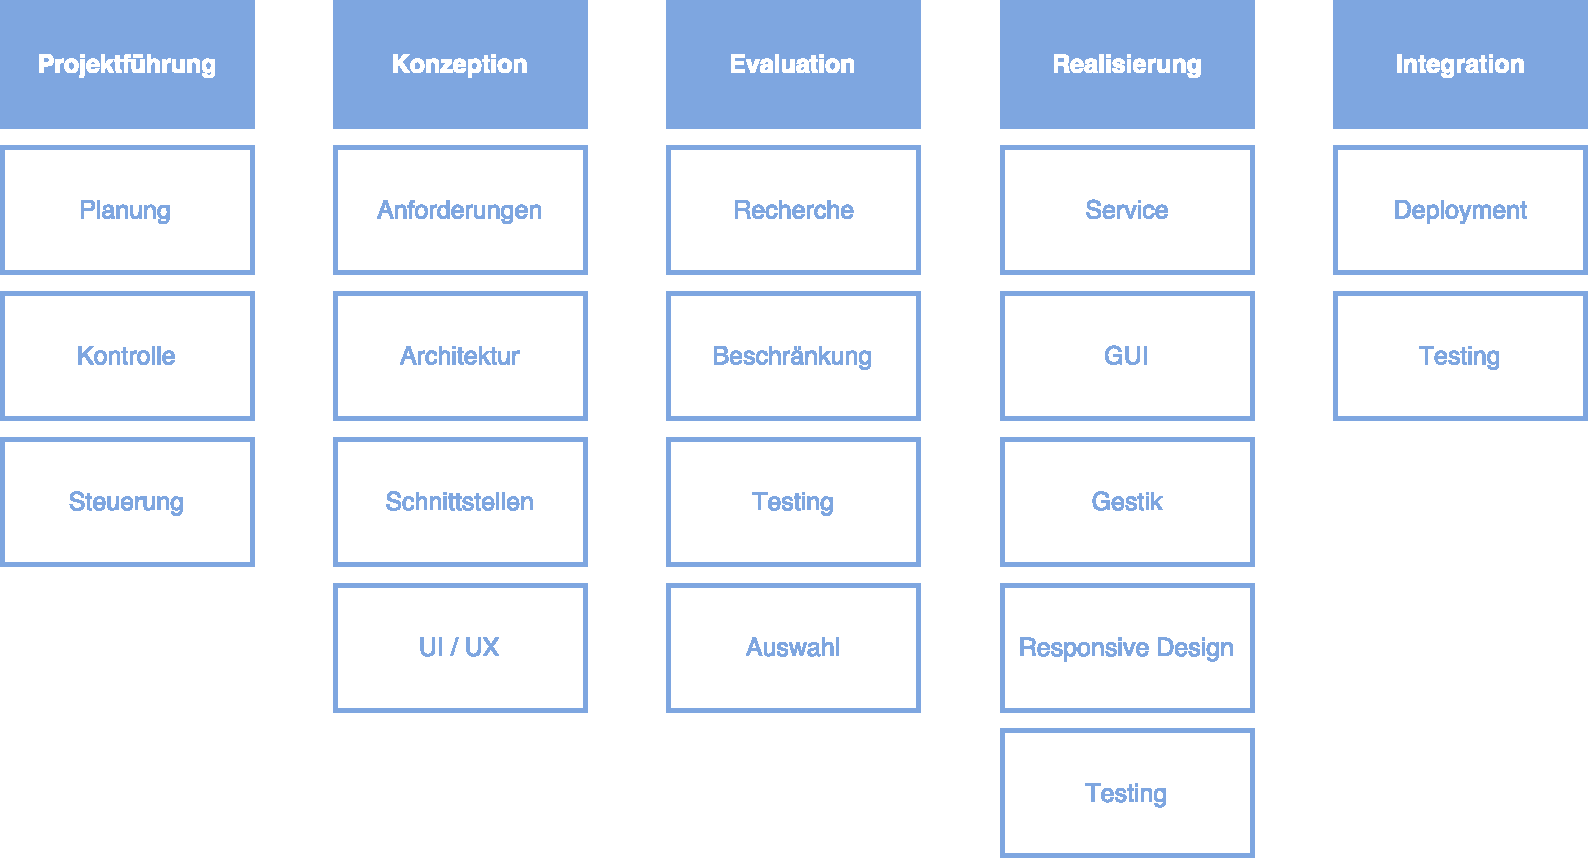
\includegraphics[width=1.5\textwidth]{Projektstrukturplan}
\caption{Projektstrukturplan}
\label{fig:projektstrukturplan}
\end{figure}
\end{landscape}

\newpage

\section{Rahmenplan}
Die Rahmenplanung, basierend auf der Projektstrukturplan (\autoref{fig:rahmenplan}), repräsentiert die zeitliche Planung des Projekts. Dabei werden Kalenderwochen anstelle von Daten oder Schulwochen verwendet. Dies kommt aufgrund des internationalen Rahmens, den damit verbundenen Zeitverschiebung und unterschiedlichen Stundenplänen. Enthalten sind alle Projektphasen, Sprints und Meilensteine, als auch alle Lieferobjekte welche im \autoref{lieferobjekte} weiter ausgeführt werden. Die Sprints haben absichtlich unterschiedliche Dauer, welche aufgrund der verschieden Projektphasen und deren Inhalt zugeordnet worden sind. Weiter werden administrative Elemente durch blaue Färbung und Entwicklungs-Elemente durch rote Färbung gekennzeichnet.

Eine grosse Rolle in der Rahmenplanung spielen die Meilensteine. Sie unterteilen das Projekt in Phasen, welche dadurch klar von einander getrennt sind. Ebenfalls sind sie eine wichtige Orientierungshilfe im Projekt und weisen den Weg damit das Projekt erfolgreich abgeschlossen werden kann. Die \autoref{tab:meilensteine} listet die Meilensteine auf.


\begin{longtable}{|p{1cm}|p{2cm}|p{8.5cm}|}
  \hline
    ID & Datum &  Beschreibung \\\hline
    M1 & 19.09.2016 & Administrativer Meilenstein, Kickoff\\\hline
    M2 & 10.10.2016 & Administrativer Meilenstein, Projektplanung abgeschlossen\\\hline
    M3 & 17.10.2016 & Entwicklung Meilenstein, Schnittstellen definiert\\\hline
    M4 & 07.11.2016 & Entwicklung Meilenstein, Evaluation Entscheid\\\hline
    M5 & 26.12.2016 & Entwicklung Meilenstein, Funktionale Oberfläche umgesetzt\\\hline
    M6 & 13.01.2017 & Entwicklung Meilenstein, Integration in \textbf{ikc-core} abgeschlossen\\\hline
    M7 & 20.01.2017 & Administrativer Meilenstein, 95\% erreicht\\\hline
    M8 & 31.01.2017 & Administrativer Meilenstein, PAWI Bericht Abgabe\\\hline
    M9 & TBD & Administrativer Meilenstein, Präsentation\\\hline
    \caption{Meilensteine}
  \label{tab:meilensteine}
\end{longtable}
\newpage

\begin{landscape}
\begin{figure}[ht]
\centering
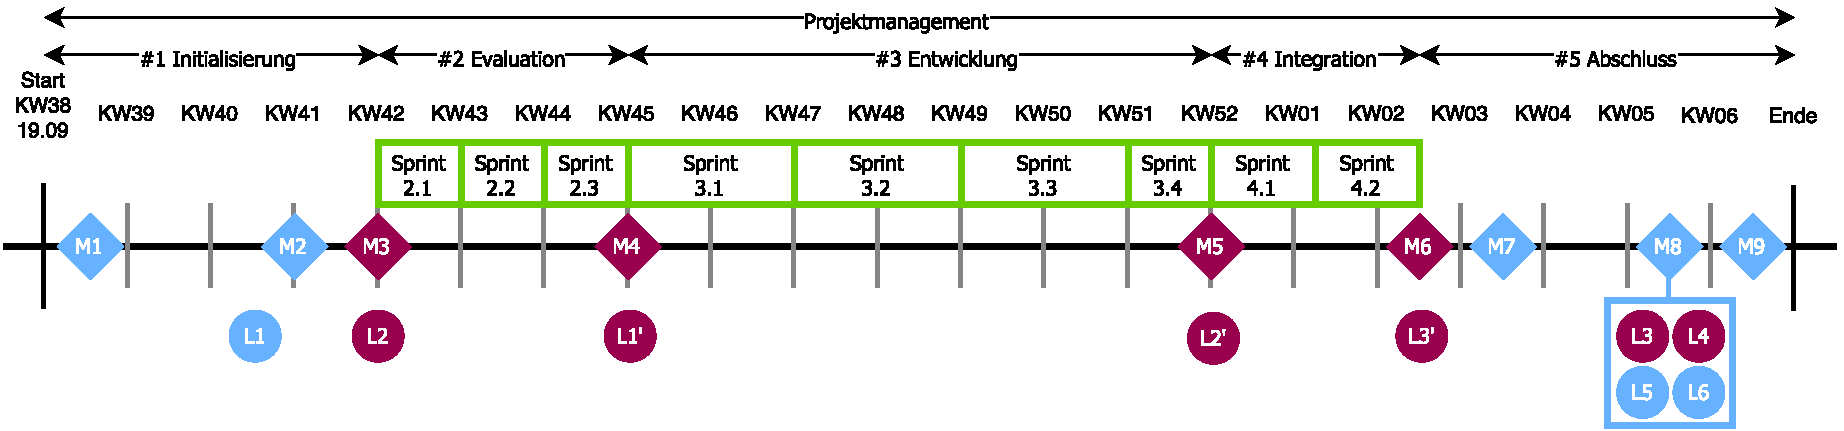
\includegraphics[width=1.7\textwidth]{Rahmenplan}
\caption{Rahmenplan}
\label{fig:rahmenplan}
\end{figure}
\end{landscape}

\newpage

\section{Projektziele} \label{projektziele}
Projektziele werden definiert, um den Projekterfolg an einigen möglichst konkreten Punkten zu messen. Diese sind in der folgenden \autoref{tab:projekt-ziele} aufgelistet.

\begin{longtable}{|p{1cm}  | p{10.5cm}|}
  \hline
    ID &  Beschreibung \\\hline
    Z1 & Ergänzung zur bestehenden Benutzeroberfläche.\\\hline
    Z2 & Intuitive, visuelle und effiziente Interaktion.\\\hline
    Z3 & Übersichtliche Visualisierung der Knoten und Kanten.\\\hline
    Z4 & Erweiterung der Funktionalität mittels Sichten (Views).\\\hline
    \caption{Projektziele}
  \label{tab:projekt-ziele}
\end{longtable}

\section{Anforderungen}

Für die weitere Unterteilung in Arbeitspakete und Stories werden die Anforderungen zunächst in Prosa gesammelt. Diese entstammen dem Kundenworkshop und der Aufgabenstellung und sind im Sinn der Projektziele (\autoref{projektziele}) ausgeführt. Die Anforderungen werden unterschieden in funktionale und nicht funktionale Anforderungen. Die funktionalen Anforderungen definieren direkt die Eigenschaften \autoref{tab:funktionale-anforderungen}. Nicht funktionale Anforderungen im Gegenteil definierten dabei die Leistung und die Randbedingungen, aufgelistet in \autoref{tab:nicht-funktionale-anforderungen}.

\begin{longtable}{|p{1.5cm} | p{1.5cm} | p{8.1cm}|}
  \hline
    ID & Priorität & Beschreibung \\\hline
    A1.1 & X & Die zugrunde liegende Datenbasis kann mittels eines Netzwerks visualisiert werden. Jenes besteht aus Knoten und Kanten, welche gerichtet und beschriftet sind. Sowohl Kanten als auch Knoten sind beschriftet.\\\hline
    A1.2 & X & Der zu erarbeitende Prototyp kann bidirektional mit dem \textit{ikc-core}-Prototypen interagieren. Änderungen am \textit{ikc-core} sind in der Visualisierung sichtbar. Es ist jedoch es auch möglich Änderungen direkt in der Visualisierung vorzunehmen.\\\hline
    A1.3 & X & Mittels der Visualisierung können die grundlegenden Datenbankoperationen \textit{CREATE}, \textit{READ}, \textit{UPDATE} und \textit{DELETE} (CRUD) teilweise direkt auf der Datenbasis des \textit{ikc-core} angewendet werden.\\\hline
    A1.3.1 & X & Es können sowohl Knoten aus dem Diagramm, als auch aus der Datenbasis gelöscht werden. Diese Vorgänge können klar unterschieden werden.\\\hline
    A1.3.2 & X & Knoten ohne Kanten können in der Visualisierung abgebildet werden.\\\hline
    A1.4 & X & Der Prototyp kann auf Smartphones und Tablets benutzt werden.\\\hline
    A1.5 & X & Der Prototyp kann auf Laptops und Desktop-Computern benutzt werden.\\\hline    
    A1.6 & X & Mit Hilfe verschiedener Kriterien (beispielsweise Kontext oder Nachbarschaft) kann ein Teilgraphen visualisiert werden.\\\hline 
    A1.6.1 & X & Diese Teilgraphen (Sichten) können unabhängig von der Datenbasis persistiert werden. Es können, zusätzlich zu den Knoten und Kanten, auch deren relative Positionen in der Visualisierung gespeichert werden.\\\hline 
    A1.7 & X & Der Prototyp kann (unter anderem) mit Drag and Drop bedient werden.\\\hline
    A1.7.1 & X & Bidirektionale und unbeschriftete Verknüpfungen zwischen visualisierten Knoten können erstellt werden.\\\hline
    A1.7.2 & X & Ein, im bestehenden User-Interface, mittels der Suche gefundener Knoten kann direkt in die Visualisierung übernommen werden.\\\hline 
    A1.7.3 & X & Ein mittels der Suchfunktion gefundener Knoten kann auf einen bestehenden Knoten gezogen werden, um mit diesem eine Kante zu bilden.\\\hline 
    A1.7.4 & X & Knoten können innerhalb des Diagramms frei positioniert werden.\\\hline 
    A1.8 & X & Die Visualisierung kann innerhalb der bestehenden \textit{ikc-core} Oberfläche genutzt werden.\\\hline 
    A1.9 & X & In der Visualisierung könnnen auch Knoten mit mehr als sieben Kindknoten dargestellt werden: Sind mehr als sieben Kindknoten vorhanden, wird anstelle einer Repräsentation jedes einzelnen Knotens auf eine Liste gewechselt. Diese Liste kann zusätzlich mit einer Such- und oder Filterfunktion versehen werden.\\\hline  
    A1.10 & X & Die von einem Knoten aus- und eingehenden Kanten können auf- und zugeklappt (sichtbar-unsichtbar) werden.\\\hline
    A1.10.1 & X & Einzelne Kanten können individuell zugeklappt / ausgeblendet werden.\\\hline
     
    \caption{Funktionale Anforderungen}
  \label{tab:funktionale-anforderungen}
\end{longtable}

\begin{longtable}{|p{1.5cm} | p{1.5cm} | p{8.1cm}|}
  \hline
    ID & Priorität & Beschreibung \\\hline
    A2.1 & X & Bestehende Komponenten des \textit{ikc-core}, wo möglich, wiederverwendet bzw. erweitert (nachhaltige Entwicklung).\\\hline
    A2.2 & X & Die Visualisierung kann in verschiedenen Projekten wiederverwendet werden.\\\hline
    A2.3 & X & Die Visualisierung wird im \textit{ikc-core} integriert (Deployment).\\\hline
    A2.4 & X & Die Visualisierung wird parallel zum \textit{ikc-core} weiterentwickelt. Die Basis für die Visualisierung bildet ein Klon des bestehenden \textit{Repositories}. Ist die Entwicklung abgeschlossen, werden die beiden Entwicklungsstände mittels eines neuen \textit{Branches} \textit{zusammengeführt} werden.\\\hline
    A2.5 & X & Jegliche Daten werden auf der Dropbox des Benutzers persistiert.\\\hline
    A2.6 & X & Es wird eine intuitive, effiziente Bedienung angestrebt. Ein Mass für die Effizienz: $\frac{\text{Taps}}{\text{Task}}$\\\hline
    A2.7 & X & Randbedingungen 180h pro Person\\\hline
    A2.8 & X & Die Arbeit können in einem Arbeitsjournal, mindestens mit Angaben von Datum, Anzahl Stunden, Arbeitsschritt/Thema, nachverfolgt werden.\\\hline
    \caption{Nicht funktionale Anforderungen}
  \label{tab:nicht-funktionale-anforderungen}
\end{longtable}

\section{Risikoanalyse}

In folgender Tabelle (\autoref{tab:risikoanalyse}) werden mögliche Risiken behandelt. Die Wahrscheinlichkeit ist mit P abgekürzt, R steht für Risiko und S für den Schaden, welcher mittels $P*R=S$ berechnet wird.


\begin{longtable}{|p{0.5cm} | p{7cm} | p{1cm}|  p{1cm}|  p{1cm}|}
  \hline
    ID & Beschreibung &  P & R & S \\\hline
    R1 & Wie in \autoref{subsec:international} bereits angesprochen wird das Projekt im \textbf{internationalen Rahmen} durchgeführt. Dies birgt einige Herausforderungen und bringt auch Riksiken mit sich: Die grösste Schwierigkeit bildet sicherlich die Zeitverschiebung. Aber auch die geographische Distanz und die lediglich im digitalen Rahmen gehaltenen Sitzungen sind nicht zu unterschätzen. Daher werden verschiedene Kommunikations-Tools angewendet, um dieser Problematik zu begegnen. & 1 & 3 & 3\\\hline
    R2 & Die Abgrenzung vom laufenden Projekt \textbf{\textit{IKC}} (vgl. \autoref{sec:scope}) ist klar festzulegen, damit es möglich wenig Überschneidungen und Unklarheiten gibt. Vollständige und detaillierte Arbeitsjournale, wie auch Protokolle bieten dabei wichtige Hilfestellung.  & 2 & 1 & 2\\\hline
    R3 & Die Zahl der Anforderungen ist verhältnismässig hoch. Im Rahmen der \textbf{360 zu leistenden Stunden} ist es wichtig sich nicht in Details oder Ausarbeitung jeglicher Finessen zu verlieren. Darum ist es umso wichtiger die Anforderungen klar zu priorisieren und auch entsprechend abzuarbeiten.  & 3 & 1 & 3\\\hline
    \caption{Risikoanalyse}
  \label{tab:risikoanalyse}
\end{longtable}

\section{Lieferobjekte}\label{lieferobjekte}

Neben den in der Aufgabenstellung vorgegebenen Lieferobjekte (\autoref{tab:set-lieferobjekte}) sind noch zusätzliche, interne Lieferobjekte (\autoref{tab:add-lieferobjekte}) festlegt. Diese sind lediglich als Unterstützung der Projektkontrolle, eine Art Orientierungshilfe, gedacht.

\begin{longtable}{|p{1cm} | p{2cm} | p{8.1cm}|}
  \hline
    ID & Datum &  Beschreibung \\\hline
    L1 & 07.10.2016 & Anforderungskatalog.\\\hline
    L2 & 17.10.2016 & Lösungskonzept inkl. Schnittstellendefinition.\\\hline
    L3 & 31.01.2017 & Funktionale Software mit folgenden Eigenschaften:
    \begin{itemize}
        \item Integriert bestehenden Prototyp auf Basis React mit allen CRUD     Funktionen \& Schnittstellen zu Dropbox und Evernote
        \item Gibt die Möglichkeit zur visuellen Interaktion mit einem 
            (Teil-)Netzwerk: Knoten können per Drag \& Drop verknüpft werden
        \item Die Applikation läuft auf dem Mobile, Tablet, Laptop und Desktop (in     Priorität der Reihenfolge) $=>$ responsive CSS Template verwenden
    \end{itemize}
    \\\hline
    L4 & 31.01.2017 & Dokumentierter Source Code (für Methoden und Parameter).\\\hline
    L5 & 31.01.2017 & Benutzerhandbuch.\\\hline
    L6 & 31.01.2017 & PAWI-Bericht.\\\hline
    \caption{Zusätzliche, interne Lieferobjekte}
  \label{tab:set-lieferobjekte}
\end{longtable}
 
\begin{longtable}{|p{1cm} | p{2cm} | p{8.1cm}|}
  \hline
    ID & Datum &  Beschreibung \\\hline
    L1' & 07.11.2016 & Abgeschlossene Evaluation der verschiedenen Frameworks zur Umsetzung der Visualisierung.\\\hline
    L2' & 26.12.2016 & Funktionale Visualisierung gemäss den funktionalen Anforderungen A1.3, A1.4, A1.5, A1.6, A1.7, A1.9 und A1.10. Bereit für die Integration in den \textit{ikc-core}.\\\hline
    L3' & 13.01.2017 & Abgeschlossene Integration der Visualisierung in den \textbf{ikc-core} und Erfüllung aller Anforderungen insbesondere A1.1, A1.2.\\\hline
    \caption{Zusätzliche, interne Lieferobjekte}
  \label{tab:add-lieferobjekte}
\end{longtable}

%\section{Epics}



%\section{Stories}


\chapter{Lösungsdesign}

Das Lösungsdesign beinhaltet die Grundlagen für die erfolgreiche Umsetzung des Prototyps. Vor der eigentlichen Implementation wird das Vorhaben auf konzeptioneller Ebene genauer betrachtet. Die Definition der Schnittstellen, besonders die Verminderung der Kopplung zwischen der Visualisierung und dem \gls{ikc-core}, ist hier ein wichtiger Punkt.


%Dieses Kapitel beinhaltet die definierten Schnittstellen sowohl die Auswahl des Frameworks für die Darstellung. Ein besonderes Augenmerk wird auf die Interaktion zwischen der Visualisierung und dem \textit{ikc-core} gelegt, besonders auf die Verminderung der Kopplung zwischen den beiden Komponenten. 

\section{User Interface Design}

Nachfolgend werden wichtige Punkte zum Umgang mit dem \gls{Netzwerk} und zur Integration der Visualisierung aufzeigt und weitergehende Überlegungen dazu dargelegt.

\subsection{Umgang mit dem Netzwerk}

Die Benutzeroberfläche orientiert sich hauptsächlich am \gls{Netzwerk}, bestehend aus \gls{Node}[s] und \gls{Link}[s]. Diese besitzen eine Beschriftung in Form des Titels oder in Form des entsprechenden \gls{Tags} (\autoref{fig:nodes-links}). Die Beschriftung kann zugunsten der Übersichtlichkeit gegebenenfalls ausgeblendet werden.

Wo immer möglich soll die Interaktion nicht über eine entfernte Schaltfläche, sondern direkt am jeweiligen Element in der Visualisierung geschehen. Ein mögliches Beispiel hierfür zeigt \autoref{fig:node-menu}. Am Knoten, wo eine Aktion vorgenommen werden soll, kann mittels eines Klicks (oder Ähnlichem) ein Kontextmenü geöffnet werden. Dieses ermöglicht der Situation entsprechende, weiterführende Funktionalitäten. Entsprechende Möglichkeiten sind auch beim Umgang mit Kanten vorstellbar.

\begin{figure}[htbp]
\centering
 \begin{subfigure}[b]{0.35\textwidth}
        \centering
        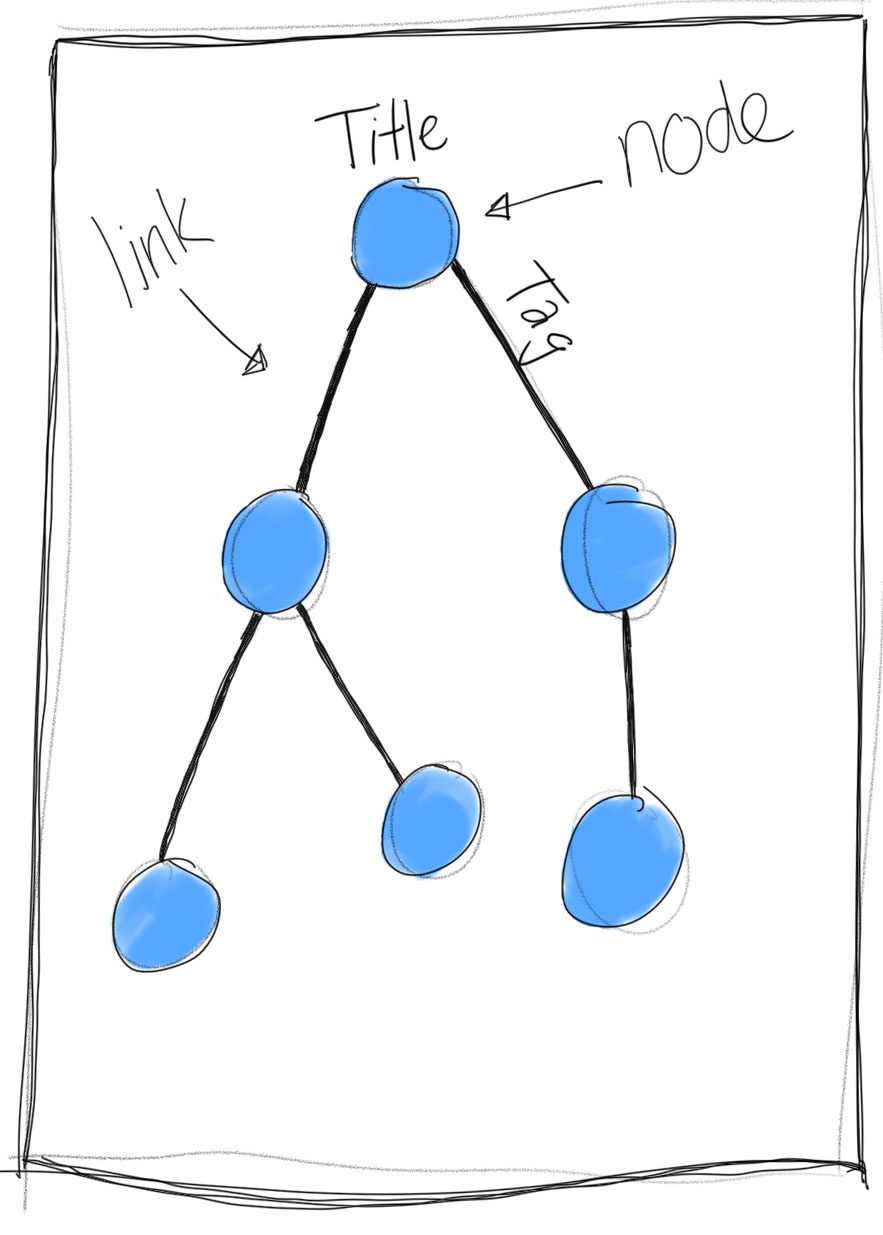
\includegraphics[width=0.9\linewidth]{skizze-nodes-links}
        \caption{Nodes und Links}
        \label{fig:nodes-links}
    \end{subfigure}
 \begin{subfigure}[b]{0.35\textwidth}
        \centering
        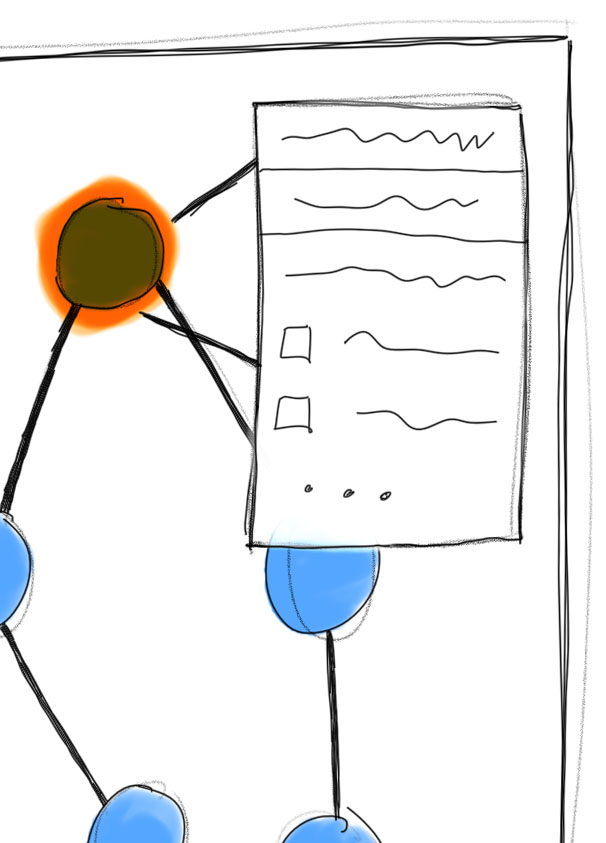
\includegraphics[width=0.9\linewidth]{skizze-contextmenu}
        \caption{Node-Menü}
        \label{fig:node-menu}
    \end{subfigure}
    \caption{Skizzen: Benutzeroberfläche}
\end{figure}


\subsection{Komponenten der Benutzeroberfläche}\label{komponenten}

Die Visualisierung verwendet Komponenten, welche Funktionen für den Benutzer zusammenfassen oder als Container für weitere Elemente dienen können. In der späteren Implementation werden diese komplett oder teilweise direkt mit einer \hyperref[react]{\textit{React}}-Komponente realisiert.

%Für die Visualisierung verwenden wir verschieden Element, in welchen Funktionen für den Benutzer zusammengefasst werden oder auch als Container für weiter Inhalte dienen. Diese werden dann in der Implementation durch eine \gls{React} Komponente oder einen Teil einer repräsentiert. 

\subsubsection{GraphScreen}
Der \textit{GraphScreen} (\autoref{fig:graph-screen-draw}) beinhaltet alle wesentlichen Elemente der Visualisierung. Dazu gehört in erster Linie das \gls{Netzwerk}, in welchem die \gls{Node}[s] und \gls{Link}[s] dargestellt werden. Weiter ist eine Navigationsleiste (\textit{Toolbar}) enthalten, in welcher wichtige Funktionen zur Verfügung gestellt werden. 

\begin{figure}[htbp]
    \centering
     \begin{subfigure}[b]{0.4\textwidth}
    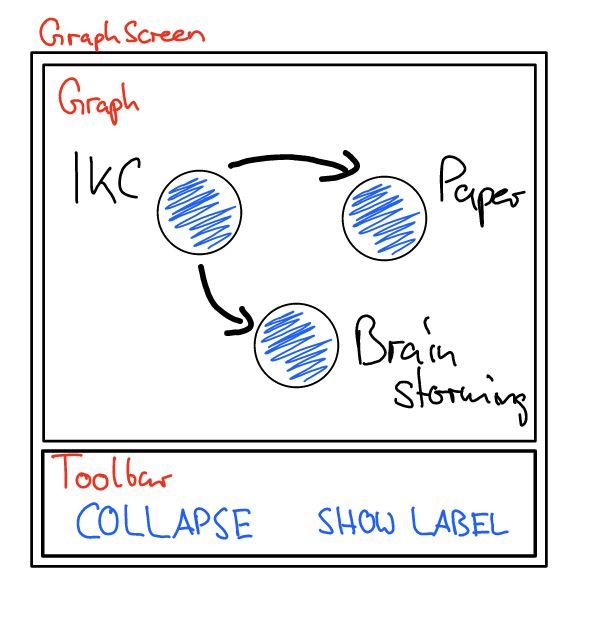
\includegraphics[width=1\linewidth]{GraphScreen}
    \caption{GraphScreen}
    \label{fig:graph-screen-draw}
    \end{subfigure}
    \begin{subfigure}[b]{0.5\textwidth}
    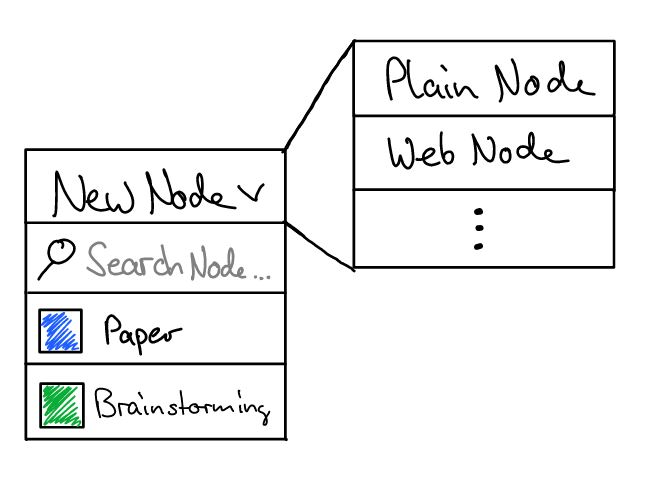
\includegraphics[width=1\linewidth]{CoreContextMenu}
    \caption{CoreContextMenu}
    \label{fig:core-context-menu}
    \end{subfigure}
    \caption{Skizzen: Benutzeroberfläche}
\end{figure}

\subsubsection{CoreContextMenu}
Das über einen \textit{Rechtsklick} (Desktop) bzw. \textit{Tap} (Mobile) zu öffnende \textit{CoreContextMenu} macht für den gegebenen Kontext weitere Funktionen abrufbar (\autoref{fig:core-context-menu}). Dabei geht es in erster Linie darum in der Visualisierung neue \gls{Node}[s] darzustellen. Einerseits können neue \gls{Node}[s] erstellt, andererseits über die Suchfunktion (auch in der Datenbasis bestehende) gefunden und verwendet werden. Der neu hinzugefügtn Knotenbefindet sich automatisch an jener Position, wo das Menü geöffnet wurde.

% So können verschiedenen Dialoge aufgerufen werden um unterschiedliche \gls{Node}[s] zu erstellen und in der Sicht darzustellen oder über ein Such Feld können bestehende Node der Sicht hinzugefügt werden. Der resultierende neue Node wird dabei an derselben Stelle dargestellt wo das Menu geöffnet wurde. Das Öffnen des Menüs erfolgt dabei durch einen \textit{Rechtsklick} (Desktop) oder \textit{Tap} (Mobile). 


\subsubsection{NodeContextMenu}
Aktionen, welche auf einen spezifischen \gls{Node} angewendet werden, sind im \textit{NodeContextMenu} zusammengefasst (\autoref{fig:node-context-menu}). Dazu zählen Aktionen, mit welchen der entsprechende \gls{Node} oder dessen \gls{Link}[s] bearbeitet werden können. Auch dieses Menü öffnet sich durch einen \textit{Rechtsklick} (Desktop) oder \textit{Tap} (Mobile). 


\begin{figure}[htbp]
\centering
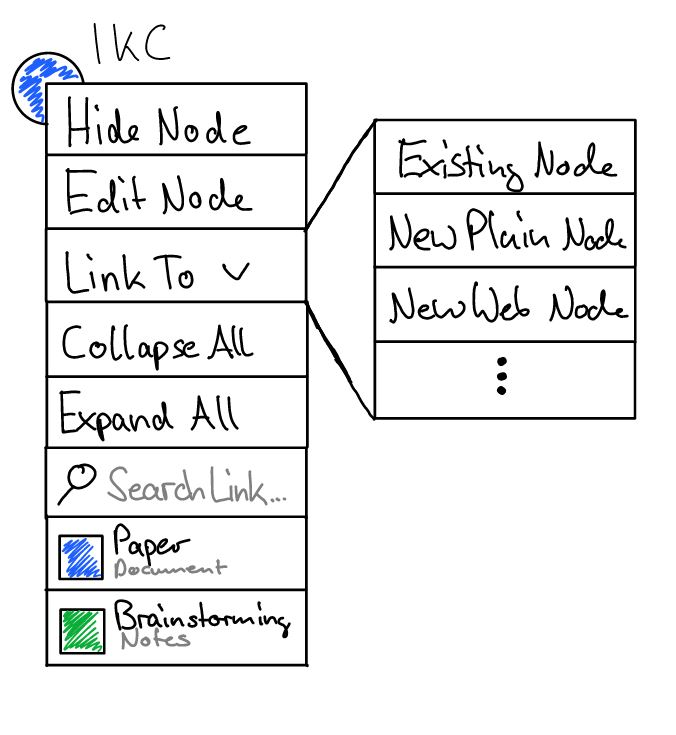
\includegraphics[width=0.5\textwidth]{NodeContextMenu}
\caption{Skizze: NodeContextMenu}
\label{fig:node-context-menu}
\end{figure}

\subsection{Aktionen}
\label{subsec:aktionen}
In einem Menu, der Toolbar oder durch ein \gls{Drag'n'Drop} können verschiedene Funktionen auf einzelne \gls{Node}[s], \gls{Link}[s] oder das gesamte \gls{Netzwerk} angewendet werden. Dazu gehören:

    \begin{longtable}{|P{2cm}|P{5cm}||p{0.3cm}|p{0.3cm}|p{0.3cm}|p{0.3cm}|p{0.3cm}|p{0.3cm}|}
  \hline
    Aktion & Beschreibung & \rotatebox[origin=c]{90}{CoreContextMenu}& \rotatebox[origin=c]{90}{NodeContextMenu}& \rotatebox[origin=c]{90}{Toolbar}& \rotatebox[origin=c]{90}{Drag'n'Drop}& \rotatebox[origin=c]{90}{Click}& \rotatebox[origin=c]{90}{Tab}\\\hline
    \textit{Edit Node} & Einen \gls{Node} bearbeiten. &&x&&&x& \\\hline
    \textit{Add Node} & Einen existierenden \gls{Node} aus der Datenbasis der Visualisierung hinzufügen. Dabei werden alle \gls{Link}[s] und deren Ziel-Nodes ebenfalls dargestellt. &x&&&x&& \\\hline
    \textit{Hide Node} & Einen \gls{Node} mit seinen \gls{Link}[s] aus der Sicht entfernen (nicht aber aus der Datenbasis). &&x&&&& \\\hline
    \textit{Delete Node} & Das Löschen eines \gls{Node}[s] aus der Sicht und der Datenbasis. Dies ist nur möglich durch die Bearbeitung des \gls{Node}[s] in der Detailansicht. &&&&&& \\\hline
    \textit{Delete Link} & Das Löschen eines \gls{Link}[s] aus der Sicht und der Datenbasis. Dies ist nur möglich durch die Bearbeitung des \gls{Node}[s] in der Detailansicht. &&&&&& \\\hline
    \textit{New Node} &  Einen neuen \gls{Node} erstellen. &x&&&&& \\\hline
    \textit{New Link} & Einen neuen \gls{Link} zwischen zwei \gls{Node}[s] erstellen. Hierzu wird ein \gls{Node} über einen anderen gezogen und losgelassen. (\autoref{fig:add-link}). &&&&x&& \\\hline
    \textit{Link To New Node} & Neuen \gls{Node} erstellen und anschliessend mit einem anderen \gls{Node} durch einen \gls{Link} verbinden. &&x&&&& \\\hline
    \textit{Link To Existing Node} & \gls{Link} zu einem existierenden \gls{Node} in der Datenbasis erstellen. &&x&&x&& \\\hline
    \textit{Collapse All} & Alle ausgehenden \gls{Link}[s] des entsprechenden \gls{Node}[s] werden zusammen mit ihren Ziel-Nodes ausgeblendet. Falls der Ziel-Node noch über andere \gls{Link}[s] verfügt, wird nur der \gls{Link} zwischen dem \gls{Node} und dem Ziel-Node ausgeblendet (\autoref{fig:collapse-all}). &&x&&&& \\\hline
    \textit{Select Link} & \gls{Link}[s] auswählen, um eine weitere Aktion auf alle anwenden zu können. &&&&&x&x \\\hline
    \textit{Collapse Links} & Ausgewählte \gls{Link}[s] werden zusammen mit ihren Ziel-Nodes ausgeblendet. Falls der Ziel-Node noch über andere \gls{Link}[s] verfügt, wird nur der \gls{Link} zwischen dem \gls{Node} und dem Ziel-Node ausgeblendet (\autoref{fig:collapse-link}). &&&x&&& \\\hline
    \textit{Expand All} & Alle ausgehenden \gls{Link}[s] eines entsprechenden \gls{Node}[s] werden zusammen mit deren Ziel-Nodes eingeblendet (\autoref{fig:expand-all}). &&x&&&& \\\hline
    \textit{Expand Link} & Einen ausgehenden \gls{Link} eines \gls{Node} darstellen. &&x&&&& \\\hline
    \textit{Show/Hide Labels} & Beschreibungen der \gls{Link}[s] darstellen oder ausblenden. &&&x&&& \\\hline
    \textit{Update Position} & Ein \gls{Node} kann neu positioniert werden. &&&&x&& \\\hline
    \caption{Funktionen}
  \label{tab:funktionen}
\end{longtable}


% \begin{figure}
%    \centering
%     \begin{subfigure}{0.4\textwidth}
%    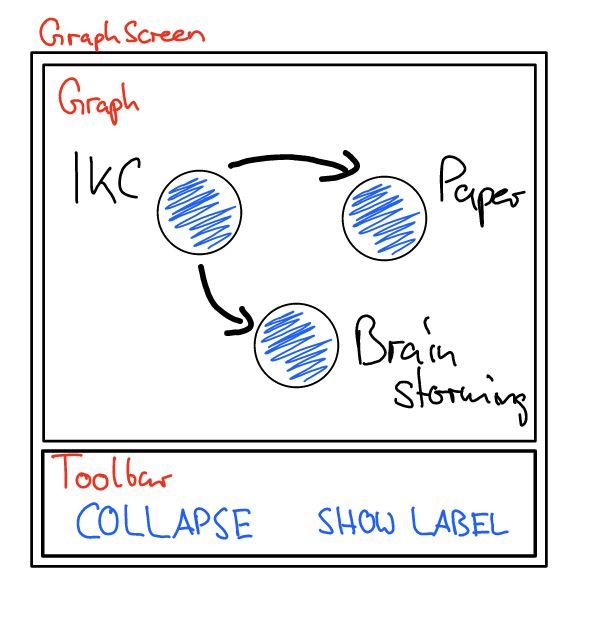
\includegraphics[width=0.9\linewidth]{GraphScreen}
%    \caption{GraphScreen}
%    \label{fig:graph-screen-draw}
%    \end{subfigure}
%    \begin{subfigure}{0.5\textwidth}
%    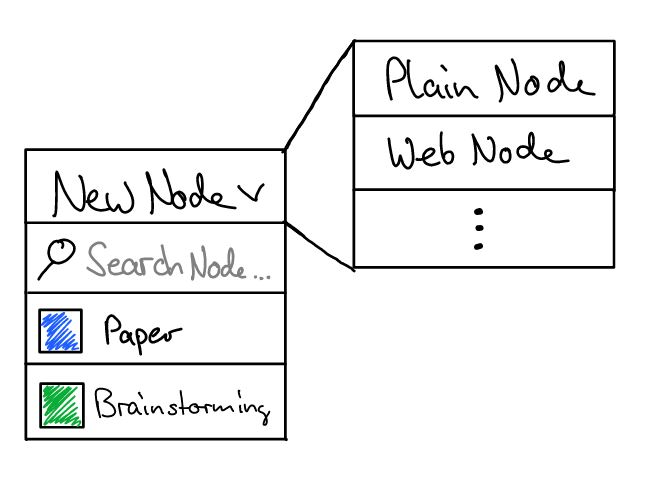
\includegraphics[width=0.9\linewidth]{CoreContextMenu}
%    \caption{CoreContextMenu}
%    \label{fig:core-context-menu}
%    \end{subfigure}
%    \caption{Skizzen Benutzeroberfläche}
%\end{figure}

\begin{figure}[htbp]
\centering
    \begin{subfigure}[b]{0.5\textwidth}
    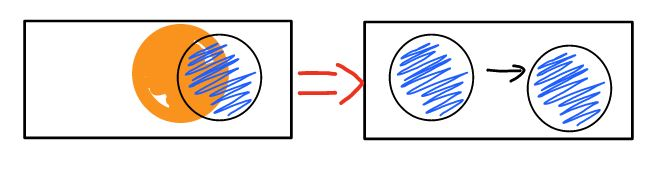
\includegraphics[width=1\linewidth]{AddLink}
    \caption{New Link}
    \label{fig:add-link}
    \end{subfigure}
    \begin{subfigure}[b]{0.4\textwidth}
    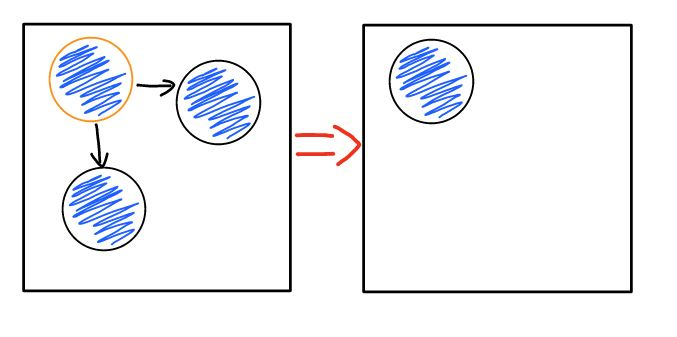
\includegraphics[width=1\linewidth]{CollapseAll}
    \caption{Collapse All}
    \label{fig:collapse-all}
    \end{subfigure}
    \caption{Skizzen: Aktionen}
\end{figure}

\begin{figure}[htbp]
\centering
    \begin{subfigure}[b]{0.4\textwidth}
    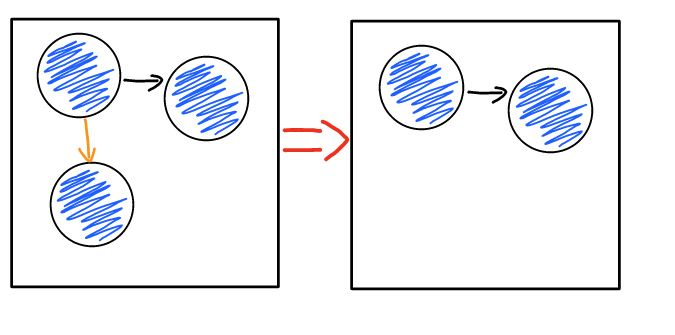
\includegraphics[width=1\linewidth]{CollapseLink}
    \caption{Collapse Link}
    \label{fig:collapse-link}
    \end{subfigure}
    \begin{subfigure}[b]{0.5\textwidth}
    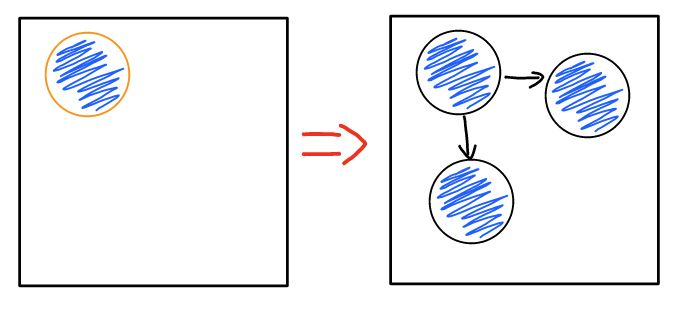
\includegraphics[width=1\linewidth]{ExpandAll}
    \caption{Expand All}
    \label{fig:expand-all}
    \end{subfigure}
    \caption{Skizzen: Aktionen}
\end{figure}


\subsection{Integration}

Aus den Anforderungen geht die Interaktion mit dem \gls{ikc-core} als weiterer wichtiger Punkt hervor. Von besonderer Bedeutung ist hier die Bedienung mittels \gls{Drag'n'Drop}. Wie in \autoref{fig:grenze-core-visual} sichtbar, muss dabei die Grenze zwischen \gls{ikc-core} und der Visualisierung (grüne Linie) überwunden werden. Mittels \gls{Drag'n'Drop} kann also beispielweise ein \gls{Node} aus der \gls{ikc-core}-Komponente (orange) in die Visualisierung positioniert werden. Dort kann dieser weiter mit dem bestehenden \gls{Netzwerk} verknüpft oder als eigenständiger neuer Knoten dargestellt werden.

\begin{figure}[htbp]
\centering
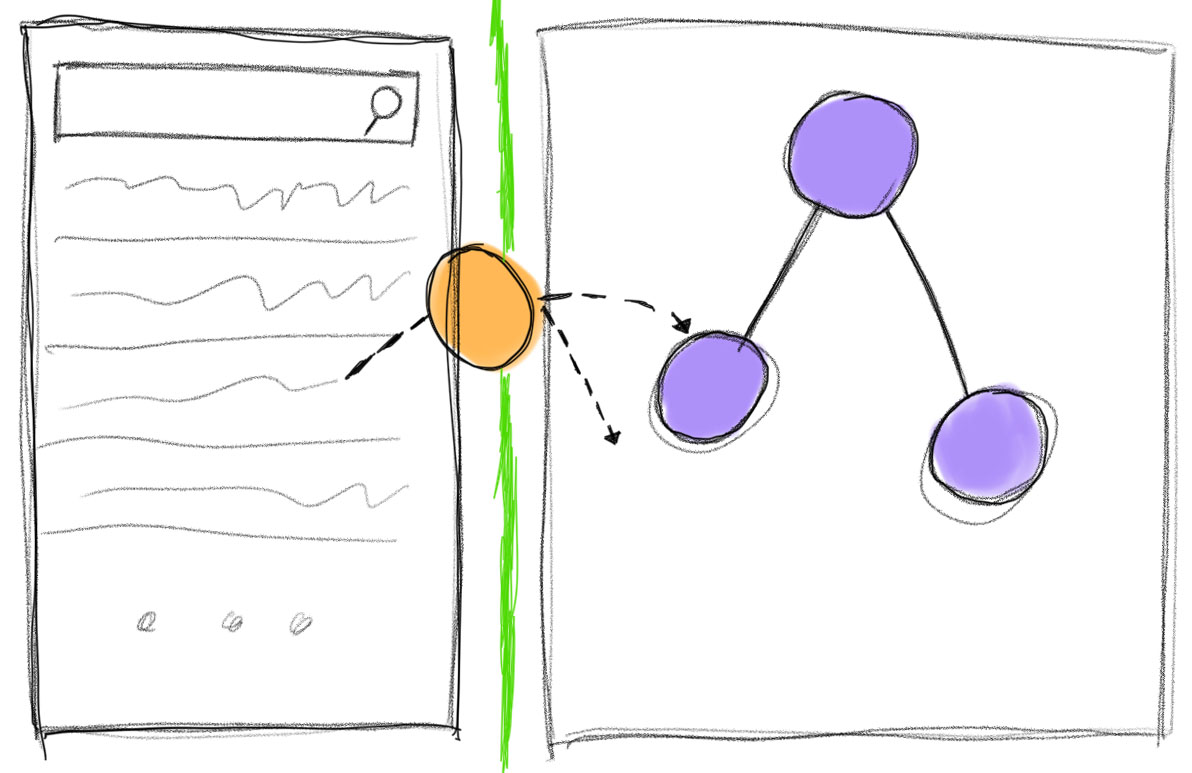
\includegraphics[width=0.5\textwidth]{ikc-core-visual}
\caption{Grenze \gls{ikc-core} - visual}
\label{fig:grenze-core-visual}
\end{figure}

Wo immer möglich, sollen bestehende Komponenten wiederverwendet werden. Dies bietet sich nicht nur bei \autoref{fig:node-menu} in Form eines Kontextmenüs, sondern auch für die Suchfunktion und die Detailansicht an. Für die Desktop-Ansicht wird die Visualisierung mittig in einer dreispaltigen Anordnung in den \textit{ikc-core} eingebettet (\autoref{fig:3-column}). Auf der linken Seite befindet sich die Suche. Auf der rechten Seite die Detailansicht für den in der Visualisierung ausgewählten \gls{Node}. Dort sind auch weitere Optionen in Form von Menüpunkten verfügbar, beispielsweise sind die ausgehenden \gls{Link}[s] erreichbar. Zu\-sätz\-lich gibt es eine übergeordnete Navigationsleiste, wo wichtige Funktion direkt abrufbar sind.

Bei der Version für Tablets und Smartphones sind, je nach verfügbarer Breite, nur eine oder zwei Spalten sichtbar.

\begin{figure}[htbp]
\centering
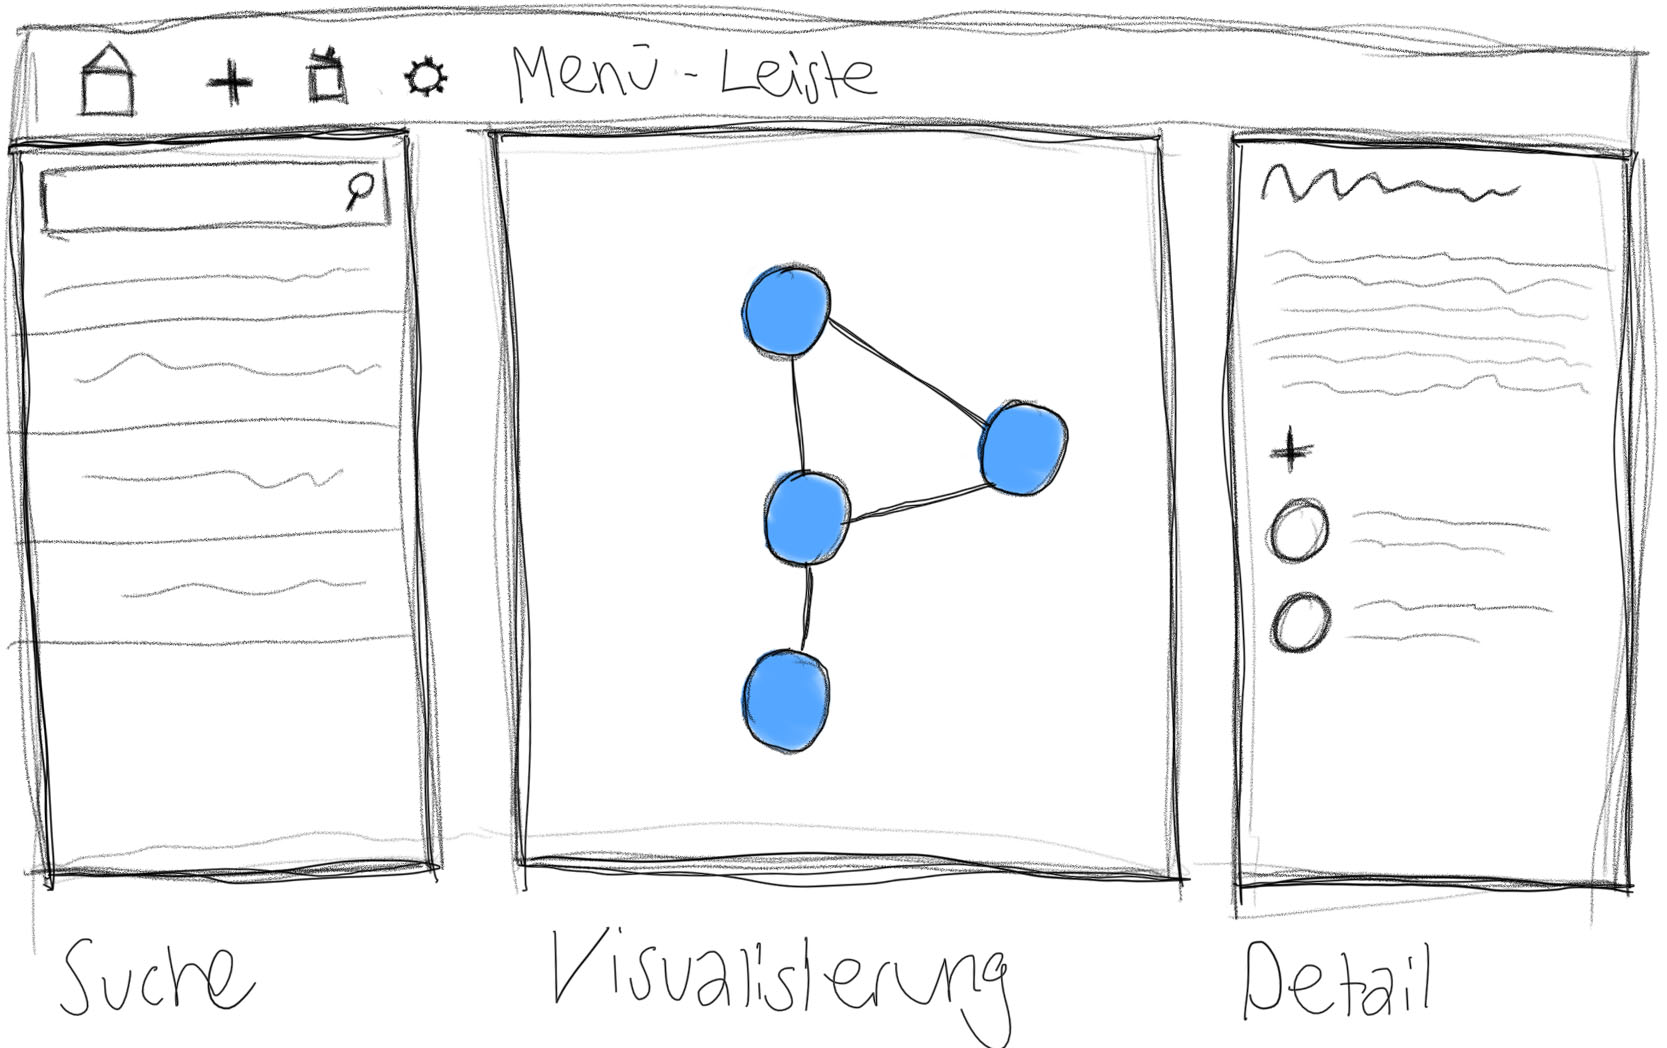
\includegraphics[width=0.8\textwidth]{integration-3-column}
\caption{3-spaltige Oberfläche}
\label{fig:3-column}
\end{figure}

\section{Technische Ausgangslage}
Der \gls{ikc-core} funktioniert momentan mit einer rudimentären Benutzeroberfläche. Die Applikationslogik und der Umgang mit der Datenbasis existieren somit bereits. Wie auf dem Komponentendiagramm (\autoref{fig:komponentendiagramm}) ersichtlich, nutzt der \gls{ikc-core} die Visualisierung (\textit{graph-visualization}). Jedoch müssen dazu verschiedene Schnittstellen der Visualisierung implementiert werden. Diese werden von der Visualisierung genutzt, um Operationen an den \gls{ikc-core} zu delegieren. Dies kann als Nutzungsvertrag zwischen der Visualisierung und der Komponente, welche sie verwendet, verstanden werden. Beispielsweise interessiert es die Visualisierung wenig, wie und wo ein \gls{Node} gespeichert wird. Es wird nur die jeweilige Methode ausgeführt, alles andere geschieht ausserhalb der Vi\-su\-ali\-si\-erung. Mehr Details dazu sind im \autoref{sec:architektur} zu finden.

\begin{figure}[htbp]
\centering
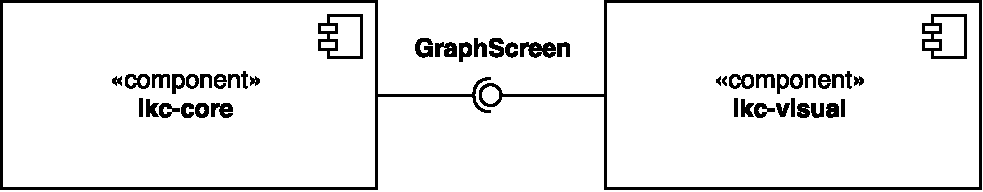
\includegraphics[width=0.6\textwidth]{components}
\caption{Komponentendiagramm}
\label{fig:komponentendiagramm}
\end{figure}

\section{Architektur}
\label{sec:architektur}

Das Klassendiagramm (\autoref{fig:klassendiagramm}) gewährt einen detaillierten Überblick über die Architektur der Visualisierung. Es zeigt die Schnittstellen zum \gls{ikc-core} und die wichtigsten Komponenten auf. Die \hyperref[react]{\textit{React}}-Klasse \textit{GraphScreen} repräsentiert das gesamte Packet ausserhalb der Visualisierung. Sie hält alle internen Klassen, Interfaces und Komponenten zusammen und stellt sicher, dass Informationen zum richtigen Zeitpunkt bei der richtigen Klasse platziert werden. \textit{Graph} als zweite grosse \hyperref[react]{\textit{React}}-Klasse kapselt das \gls{Framework} \textit{cytoscape} und stellt die Interaktion mit der Visualisierung sicher. Die weiteren Schnittstellen, Klassen und ihre Implementationen werden im \autoref{schnittstellen}, \autoref{model} und \autoref{implementation} genauer ausgeführt.

\begin{landscape}
\begin{figure}[htbp]
\centering
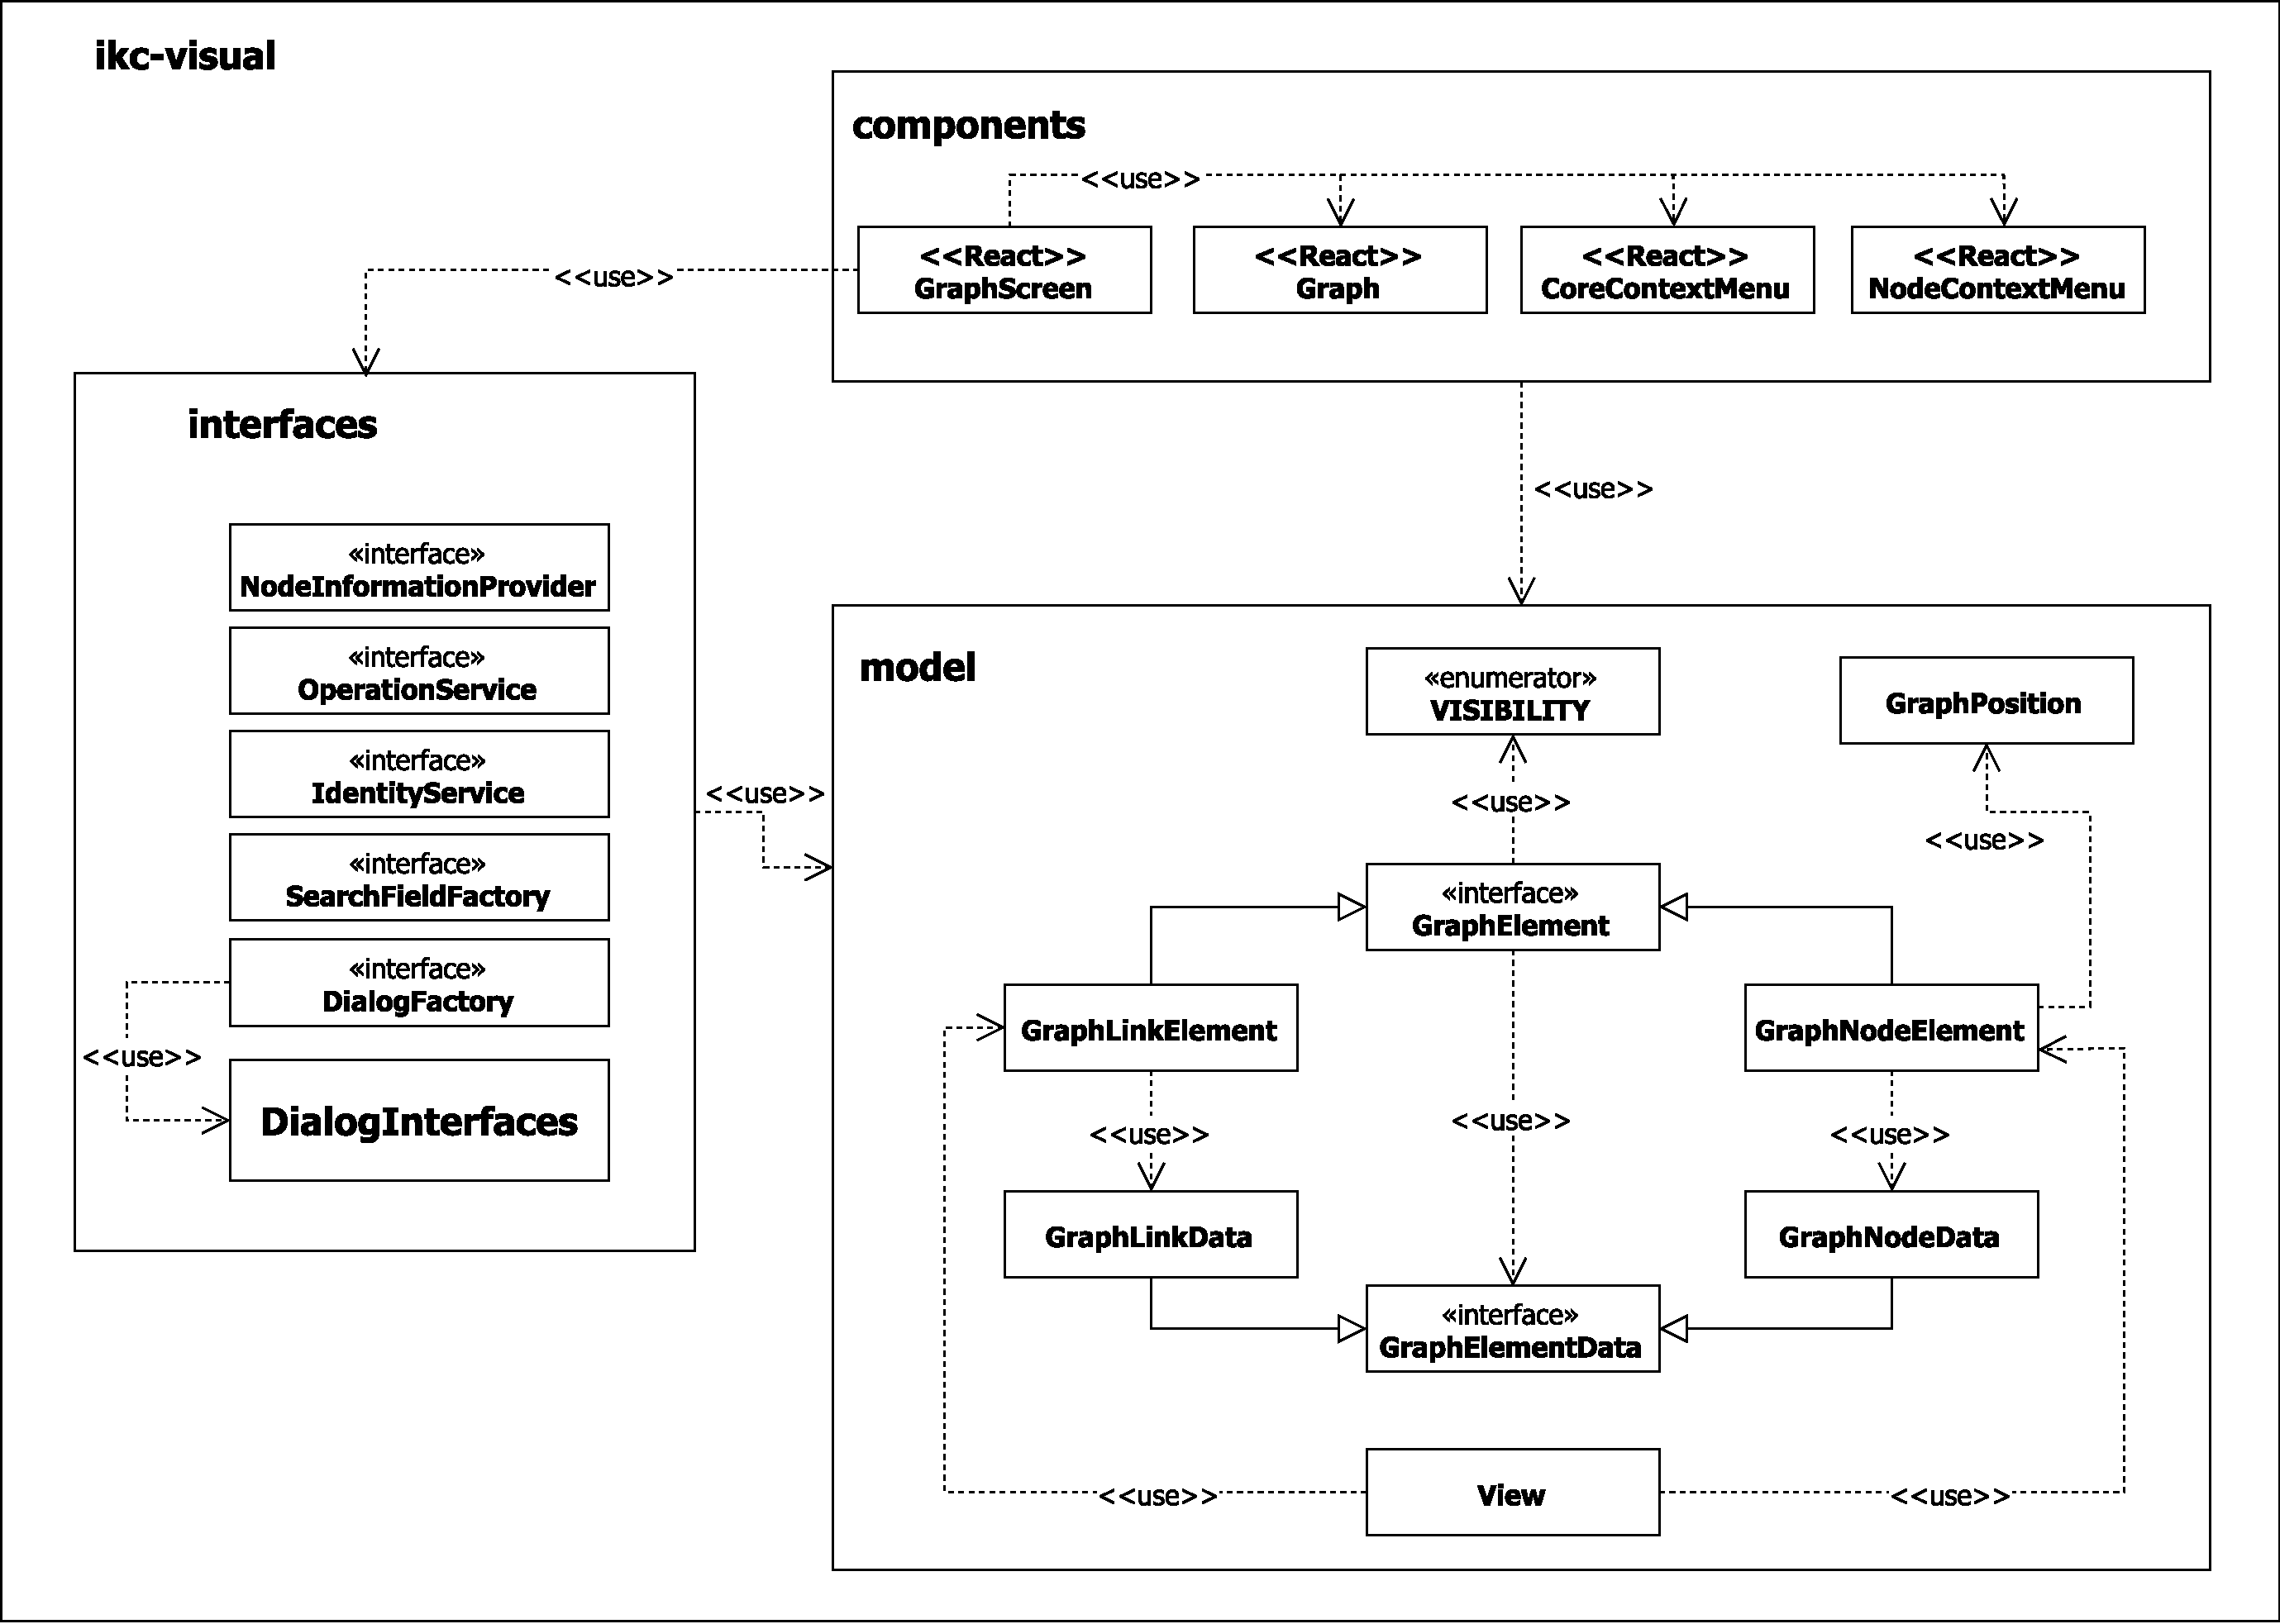
\includegraphics[width=1.6\textwidth]{architecture-overview}
\caption{Klassendiagramm}
\label{fig:klassendiagramm}
\end{figure}
\end{landscape}

\section{Schnittstellen} \label{schnittstellen}

Die hier gezeigten Schnittstellen dienen dem Austausch und der Interaktion mit dem \textit{ikc-core}. Um die Visualisierung in einer bestehenden Umgebung zu verwenden, müssen die erforderlichen Teile implementiert werden.

Die \autoref{fig:integration-ikc-core} zeigt einen Teil einer möglichen Integration, beispielsweise in den bestehenden \gls{ikc-core}. Die rechte Seite stellt einen Ausschnitt des \textit{ikc-visual}-Paketes an. Die Klasse \textit{GraphScreen} (\autoref{GraphScreenProps}) ist zu\-stä\-ndig für die Visualisierung des \gls{Netzwerk}[s]. Um den vollen Funktionsumfang zu bieten, benutzt sie, unter anderem, die Schnittstelle \textit{DialogFactory} (\autoref{DialogFactory}). Diese soll den Umgang mit Dialogfenstern ermöglichen. Da dies zu den grundlegenden Funktionen der Visualisierung zählt, befindet sich diese Schnittstelle direkt im \textit{ikc-visual}-Paket. Bei der Integration der Visualisierung in eine bestehende Umgebung gilt es somit, alle Schnittstellen entsprechend zu implementieren.

Die Klasse \textit{GraphVisualisation} verwendet die Klasse \textit{GraphScreen} aus der Visualisierung. Folglich muss beispielsweise die Schnittstelle \textit{DialogFactory} implementiert werden. Dies wird mit der Klasse \textit{GraphDialogFactory} realisiert.

Ähnlich wie beim oben beschriebenen Beispiel gibt es weitere Voraussetzungen des \textit{GraphScreen}, welche bei einer Integration beachtet werden sollten. Diese werden nachfolgend genau erläutert.

Es folgt eine Beschreibung der im \textit{ikc-visual}-Paket enthaltenen Klassen und Schnittstellen. 
\begin{figure}[htbp]
\centering
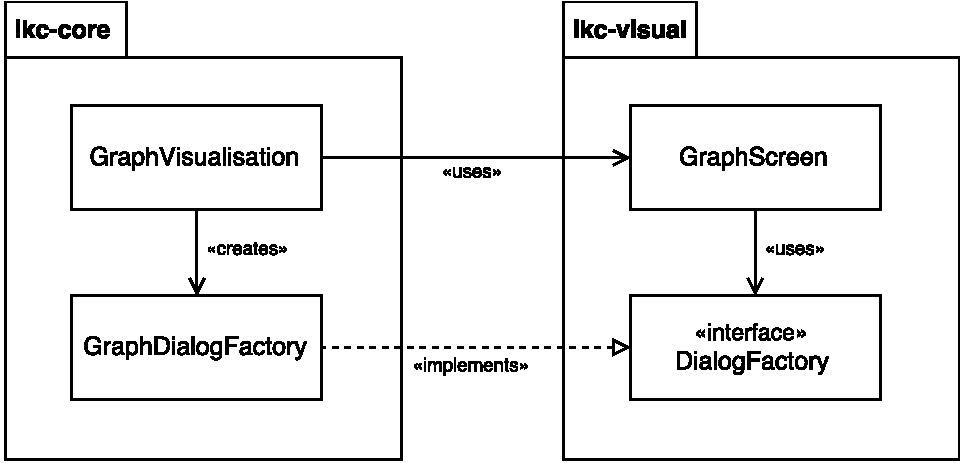
\includegraphics[width=0.7\textwidth]{architecture}
\caption{Integration \gls{ikc-core}}
\label{fig:integration-ikc-core}
\end{figure}

\subsection{GraphScreenProps}\label{GraphScreenProps}
Die \hyperref[react]{\textit{React}}-Komponente \textit{GraphScreen} wird seitens der Visualisierung implementiert. Sie ist die einzige, welche ausserhalb der Visualisierung genutzt werden kann. Damit ist deren Nutzung gleichzustellen mit der Nutzung der Visualisierung. Mit Hilfe der Schnittstelle \textit{GraphScreenProps} wird geregelt, wie die Komponente genutzt werden kann und welche Informationen, respektive welche Implementationen ihr zur Verfügung gestellt werden müssen.  

Somit sammelt die \textit{GraphScreen}-Komponente alle Abhängigkeiten und repräsentiert das \gls{Netzwerk} als Ganzes. Sie hält alle Referenzen zu Daten, Funktionen, sowie zu den umliegenden Komponenten. Damit stellt sie das einzige Bindeglied zwischen \gls{ikc-core} und der Visualisierung dar. Für die Verwendung der Komponente sind die folgenden Objekte bereitzustellen: Ein grosser Teil in Form von Implementationen von Schnittstellen, welche in der Visualisierung definiert sind. Diese werden in den nächsten Abschnitten genauer erläutert (\autoref{listing:graphscreen}):

\begin{itemize}
    \item \textit{viewToLoad} - View, welche angezeigt wird.
    \item \textit{nodeInformationProvider} - Stellt weitere Informationen zu \gls{Node}[s] und \gls{Link}[s] zur Verfügung.
    \item \textit{operationService} - Ermöglicht Interaktion mit der Datenbasis.
    \item \textit{timestamp} - Timestamp der letzten Verwendung.
    \item \textit{dialogFactory} - Ermöglicht den Zugriff auf die verschiedenen Dialoge.
    \item \textit{searchFieldFactory} - Ermöglicht den Zugriff auf die verschiedenen Suchfelder.
    \item \textit{onNodeDetailRequest} - \gls{Callback}-Methode, wenn weitere Informationen zu einem \gls{Node} gewünscht sind.
    \item \textit{nodeTypes} - Eine Liste verschiedener Arten von \gls{Node}[s], z.B. \textit{Plain}, \textit{Dropbox}, etc.
    \item \textit{identityService} - Ermöglicht das Erstellen von eindeutigen Indentifikationsnummern für neu erstellte \gls{Node}[s] und \gls{Link}[s]
\end{itemize}

\begin{listing}[htbp]
\inputminted[
frame=lines,
framesep=2mm,
baselinestretch=1.2,
linenos,
breaklines=true
]{js}{sourcecode/common/interfaces/GraphScreenProps.ts}
\caption{GraphScreen-Komponente}
\label{listing:graphscreen}
\end{listing}

In \autoref{listing:graphscreenexample} ist ein Beispiel für die Verwendung aufgezeigt. 

\begin{listing}[htbp]
\inputminted[
frame=lines,
framesep=2mm,
baselinestretch=1.2,
linenos,
breaklines=true
]{js}{sourcecode/GraphScreenExample.tsx}
\caption{GraphScreen-Beispiel}
\label{listing:graphscreenexample}
\end{listing}


\subsection{NodeInformationProvider}
\label{NodeInformationProvider}

Die Visualisierung benötigt für die Darstellung des \gls{Netzwerk}[s] diverse Informationen zu den einzelnen \gls{Node}[s] und \gls{Link}[s]. Dazu bietet der \textit{NodeInformationProvider} die beiden Methoden \texttt{getNodeTitle} und \texttt{getLinkLabel}. Die Identifikation erfolgt jeweils über eine eindeutige Identifikationsnummer (ID) (\autoref{listing:nodeinformationprovider}).

Teile der Visualisierung sollen mittels \gls{Drag'n'Drop} bedient werden können. Folgend ein Beispiel, wie die Schnittstelle in diesem Anwendungsfall benutzt werden kann:

Für ein \textit{Drag and Drop} wird üblicherweise ein \gls{Event} beim Loslassen des gepackten Elements ausgelöst. Das Element soll eine eindeutige ID enthalten. Dies ist aus dem bestehenden \textit{IKC-Core} vorausgesetzt. Wird das Element nun innerhalb der Visualisierung losgelassen, enthält der ausgelöste \gls{Event} diese ID. Sie wird zusammen mit dem \gls{Event} abgefangen und kann weiterverwendet werden. Beispielsweise können nun Informationen über den \textit{NodeInformationProvider} bezogen werden.

\begin{listing}[htbp]
\inputminted[
frame=lines,
framesep=2mm,
baselinestretch=1.2,
linenos,
breaklines=true
]{js}{sourcecode/common/interfaces/NodeInformationProvider.ts}
\caption{NodeInformationProvider-Interface}
\label{listing:nodeinformationprovider}
\end{listing}

Diese Schnittstelle deckt alle Leseoperationen ab. Schreiboperationen sind in der Schnittstelle \textit{OperationService} (\autoref{listing:operationservice}) zusammengefasst und werden im nächsten Abschnitt ausgeführt. 

\subsection{OperationService}
\label{OperationService}

Die \textit{OperationService}-Schnittstelle ermöglicht der Visualisierung Operationen an die Datenbasis weiterzuleiten. Damit spezifiziert und bün\-delt diese Schnittstelle alle Schreiboperationen, welche vom \gls{ikc-core} implementiert werden müssen (\autoref{listing:operationservice}). Diese Operationen entsprechen den folgenden vier Methoden:

\begin{enumerate}
  \item \texttt{createNodeFromDialogState} - neuer \gls{Node} auf der Basis des \textit{NewNode} Dialogs.
  \item \texttt{createNodeWithLinkFromDialogState} - neuer \gls{Node}, zusammen mit einem \gls{Link} zu einem bestehenden \gls{Node}, auf der Basis des \textit{NewNodeToConnect} Dialogs.
  \item \texttt{createLink} - neuer \gls{Link} definiert durch \textit{id}, den beiden \gls{Node}[s] \textit{source} und \textit{target} und dem entsprechenden \textit{label}.
  \item \texttt{saveView} - speichert die übergebene \gls{View}.
\end{enumerate}

\begin{listing}[htbp]
\inputminted[
frame=lines,
framesep=2mm,
baselinestretch=1.2,
linenos,
breaklines=true
]{js}{sourcecode/common/interfaces/OperationService.ts}
\caption{OperationService-Interface}
\label{listing:operationservice}
\end{listing}

\subsection{IdentityService}
\label{IdentityService}

Jeder \gls{Node} und jeder \gls{Link} in der Visualisierung als auch in der zugrundeliegenden Datenbasis verfügt über eine ID. Diese ermöglicht es, das Element eindeutig zu identifizieren und Operationen korrekt auszuführen. So kann ein konsistenter Kontext gewährleistet werden. Neue Elemente, welche aus der Visualisierung entstehen, müssen ebenfalls mit einer korrekten ID versehen werden. Dazu bietet die Schnittstelle \textit{IdentityService} (\autoref{listing:identityservice}) die beiden Methoden \texttt{create\-New\-Node\-Id} und \texttt{createNewLinkId}.

\begin{listing}[htbp]
\inputminted[
frame=lines,
framesep=2mm,
baselinestretch=1.2,
linenos,
breaklines=true
]{js}{sourcecode/common/interfaces/IdentityService.ts}
\caption{IdentityService-Interface}
\label{listing:identityservice}
\end{listing}

\subsection{DialogFactory}
\label{DialogFactory}
Durch die Entkopplung der Erstellung von Dialogen und der Visualisierung ist es möglich, die Visualisierung sehr flexibel einzusetzen. Die Visualisierung definiert zwar, welche Dialoge existieren, deren Implementation wird aber komplett ausgelagert. Diese Implementation ist für die Visualisierung nur soweit bedeutsam, als dass sie die benötigten Informationen liefert. Die Dialog-Schnittstellen definieren die dazu nötigen Eigenschaften. Diese Spezifikationen werden dann vom \gls{ikc-core} für die Implementation verwendet. Die verschiedenen Schnittstellen werden im nächsten \autoref{subsec:dialoginterfaces} detailliert behandelt.

%Mittels der Entkopplung, der Erstellung der nötigen Dialoge von der Visualisierung, wird ermöglicht die Visualisierung mit hoher Flexibilität zu verwenden. Die Visualisierung definiert welche Dialoge es gibt, wie diese jedoch konkret implementiert sind für die Visualisierung nicht bedeutsam solange diese die benötigen Informationen liefern. Dazu werden die Dialog Schnittstellen definiert und dadurch die zwingenden Eigenschaften der Dialoge. Diese Spezifikationen werden dann von dem \gls{ikc-core} für die Implementation verwendet. Die verschiedenen Schnittstellen werden im nächsten \autoref{subsec:dialoginterfaces} detailliert behandelt.\\
Mit Hilfe der Implementierung des \textit{DialogFactory}-Interfaces kann die Visualisierung die entsprechenden Dialoge erstellen und mit den nöt\-igen \gls{Callback} Methoden ausstatten. Dies funktioniert auch im Falle, dass die Implementation für die Visualisierung gänzlich unbekannt ist. Dabei handelt es sich um drei Dialoge, welche über separate Methoden adressiert werden können:

\begin{enumerate}
  \item \texttt{getDialogNodeNewNode} - liefert einen \textit{NewNode}-Dialog.
  \item \texttt{getDialogNodeNewNodeToConnect} - liefert einen \textit{New\-Node\-To\-Con\-nect}-Dialog.
  \item \texttt{getDialogNodeSearchToCon\-nect} - liefert einen \textit{Search\-Node\-To\-Con\-nect}-Dialog.
\end{enumerate}

\begin{listing}[htbp]
\inputminted[
frame=lines,
framesep=2mm,
baselinestretch=1.2,
linenos,
breaklines=true
]{js}{sourcecode/common/interfaces/DialogFactory.ts}
\caption{DialogFactory-Interface}
\label{listing:dialogfactory}
\end{listing}

\subsection{Dialog-Schnittstellen}
\label{subsec:dialoginterfaces}
Wie bereits aufgezeigt, übernehmen die Dialog Schnittstellen die Aufgabe, die minimalen Eigenschaften der verschiedenen Dialoge zu spezifizieren. Dies wird erreicht indem diese Schnittstellen als \textit{State}- und \textit{Props}-Interface verwendet werden.
%In den entsprechenden \hyperref[react]{\textit{React}} Implementierungen der Dialoge. 
Bei Bedarf können diese erweitert werden, um sie dem Kontext entsprechen anzupassen. Auf diese Weise wird erreicht, dass die Visualisierung die benötigten Informationen erhält. Diese Informationen nutzt sie danach, um die resultierenden Operationen der Dialoge auszuführen.

\subsubsection{NewNodeDialog}
Mittels des \textit{NewNode}-Dialogs wird es ermöglicht im \gls{ikc-core} einen Dialog zu nutzen, welcher dann seine Resultate direkt an die Visualisierung liefert. Die Schnittstelle \textit{DialogNewNodeProps} fungiert dabei als \textit{Props}-Interface. Mittels der Eigenschaft \texttt{type} wird der entsprechende Typ des zu erstellenden \gls{Node}[s] übergeben. Als Datencontainer (\texttt{node}) wird die Klasse \textit{GraphNodeElement} verwendet. Über die beiden \gls{Callback}-Methoden \texttt{on\-Request\-Close} und \texttt{onSave} wird die Visualisierung über die Endbedingungen des Dialogs informiert. In der Schnittstelle \texttt{DialogNewNodeState} wird der aktuelle Status des Dialogs gespeichert und schliesslich mit der Methode \texttt{onSave} an die Visualisierung übergeben. Dort kann der Status weiterverarbeitet werden.

\begin{listing}[htbp]
\inputminted[
frame=lines,
framesep=2mm,
baselinestretch=1.2,
linenos,
breaklines=true
]{js}{sourcecode/common/interfaces/DialogNewNodeInterfaces.ts}
\caption{DialogNewNode-Schnittstellen}
\label{listing:dialognewnode}
\end{listing}

\subsubsection{NewNodeToConnectDialog}
\label{NewNodeToConnectDialog}
Nebst der Erstellung eines \gls{Node}[s] soll es auch ermöglicht werden, mit Hilfe eines Dialogs einen neuen \gls{Node} zu erstellen, welcher mittels eines \gls{Link}[s] mit einem bestehenden \gls{Node} verbunden ist. Hierzu werden zwei zusätzliche Schnittstellen definiert: \textit{Dialog\-New\-Node\-To\-Con\-nect\-Props} und \textit{Dialog\-New\-Node\-To\-Con\-nect\-State}. Im Gegensatz zu den Schnittstellen des \textit{NewNodeDialog} wird hier als Datencontainer (\texttt{link}) für die Visualisierung die Klasse \textit{GraphLinkElement} verwendet.

\begin{listing}[htbp]
\inputminted[
frame=lines,
framesep=2mm,
baselinestretch=1.2,
linenos,
breaklines=true
]{js}{sourcecode/common/interfaces/DialogNewNodeToConnectInterfaces.ts}
\caption{DialogNewNodeToConnect-Interfaces}
\label{listing:dialognewnodetoconnect}
\end{listing}

\subsubsection{DialogNodeSearchToConnectInterfaces}
\label{DialogNodeSearchToConnectInterfaces}

Der dritte Dialog dient dazu, einen \gls{Node} aus der bestehenden Datenbasis zu suchen und diesen mit einem existierenden \gls{Node} in der Visualisierung mittels eines \gls{Link} zu verknüpfen. Wiederum werden die Eigenschaften dieses Dialogs mithilfe zweier Schnittstellen definiert: \textit{Dialog\-Node\-Search\-To\-Con\-nect\-Props} stellt wiederum sicher, dass die benötigten \gls{Callback}-Methoden zur Verfügung stehen. \textit{Dialog\-Node\-Search\-To\-Con\-nect\-State} sorgt dafür, dass die richtigen Informationen an die Visualisierung übergeben werden.

\begin{listing}[htbp]
\inputminted[
frame=lines,
framesep=2mm,
baselinestretch=1.2,
linenos,
breaklines=true
]{js}{sourcecode/common/interfaces/DialogNodeSearchToConnectInterfaces.ts}
\caption{DialogSearchNodeToConnect-Interfaces}
\label{listing:dialogsearchnodetoconnect}
\end{listing}


\subsection{SearchFieldFactory}
\label{SearchFieldFactory}
Sowohl das \textit{CoreContextMenu} als auch das \textit{NodeContextMenu} sind Komponenten, welche die Visualisierung liefert. Die integrierte Suche kann jedoch nicht von ihr zur Verfügung gestellt werden, da sie keinen Zugriff auf die zugrundeliegende Datenbasis hat%, insbesondere nicht auf die potentiell unterschiedlichen Suchalgorithmen
. Dazu wird die \textit{SearchFieldFactory} Schnittstelle verwendet, welche Zugriffe auf das \textit{NodeSearchField} und das \textit{LinkSearchField} regelt. Auch hier wird die konkrete Implementation der Suchkomponenten im \gls{ikc-core} erledigt.

Die einzelnen Komponenten werden über die Methoden \texttt{get\-Node\-Search\-Field} und \texttt{getLinkSearchField} geliefert. Dazu muss bei beiden eine \gls{Callback}-Methode übergeben werden, welche bei der Auswahl eines Suchresultats ausgeführt wird. Bei der Methode \texttt{get\-Link\-Search\-Field} muss zusätzlich ein \gls{Array} von den Link-IDs mitgeliefert werden. Darüber werden die Elemente festgelegt, welche bei der Suche berücksichtigt werden sollen.

\begin{listing}[htbp]
\inputminted[
frame=lines,
framesep=2mm,
baselinestretch=1.2,
linenos,
breaklines=true
]{js}{sourcecode/common/interfaces/SearchFieldFactory.ts}
\caption{SearchFieldFactory-Schnittstelle}
\label{lst:searchfieldfactory}
\end{listing}

\section{Model}\label{model}
Klassen oder Schnittstellen, welche sich auf die Haltung von Daten beschränken, %oder Enumeratoren 
werden als \textit{Model} zusammengefasst. So repräsentieren sie zum Beispiel eine Koordinate, einen Knoten oder einen Link. Da sie kein konkretes Verhalten implementieren, werden sie bereits im Lösungsdesign definiert. In anderen Sprachen, wie zum Beispiel \gls{Scala}, werden sie auch als sogenannte \textit{Case Classes} bezeichnet (\citep{caseClass}).

\subsubsection{GraphElement}
\label{GraphElement}
Die Schnittstelle \textit{GraphElement} ist das grundlegende Interface von \gls{Node}[s] und \gls{Link}[s]. Es wird durch zwei Eigenschaften spezifiziert (\autoref{lst:model-graphelement}):

\begin{itemize}
  \item \texttt{data} - enthält die nötigen Informationen zum jeweiligen Element. 
  %Die konkreten Klassen an dieser Stelle müssen die Schnittstelle \hyperref[GraphElementData]{\textit{GraphElementData}} implementieren um die Abstraktion dieser Schnittstelle sicherzustellen.
  \item \texttt{visibility} - beschreibt die Sichtbarkeit des Elements.
\end{itemize}

\begin{listing}[htbp]
\inputminted[
frame=lines,
framesep=2mm,
baselinestretch=1.2,
linenos,
breaklines=true
]{js}{sourcecode/common/model/GraphElement.ts}
\caption{GraphElement-Schnittstelle}
\label{lst:model-graphelement}
\end{listing}

\subsubsection{GraphElementData}
\label{GraphElementData}
Mit der einzigen Eigenschaft \texttt{id}, sorgt die Schnittstelle \textit{GraphElementData} für eine eindeutige Identifikation aller Elemente (\autoref{lst:model-graphelementdata}). 

\begin{listing}[htbp]
\inputminted[
frame=lines,
framesep=2mm,
baselinestretch=1.2,
linenos,
breaklines=true
]{js}{sourcecode/common/model/GraphElementData.ts}
\caption{GraphElementData-Interface}
\label{lst:model-graphelementdata}
\end{listing}

\subsubsection{GraphNodeElement}
\label{GraphNodeElement}
Die Klasse \textit{GraphNodeElement} repräsentiert einen einzelnen \gls{Node} und implementiert die Schnittstelle \hyperref[GraphElement]{\textit{GraphElement}}. Diese wird mit der Eigenschaft \texttt{position} erweitert, welche die aktuelle Position innerhalb der Visualisierung enthält und \texttt{nodeClasses}, um potentielle Node-Klassen zu speichern. Ebenfalls nutzt diese Klasse die entsprechende \hyperref[GraphElementData]{\textit{GraphElementData}} Implementierung \hyperref[GraphNodeData]{\textit{GraphNodeData}} . Ein \textit{GraphNodeElement} hat immer auch die gleiche ID und Titel wie in der Datenbasis, die restlichen Eigenschaften unterscheiden sich jedoch (\autoref{lst:model-graphnodeelement}).

\begin{listing}[htbp]
\inputminted[
frame=lines,
framesep=2mm,
baselinestretch=1.2,
linenos,
breaklines=true
]{js}{sourcecode/common/model/GraphNodeElement.ts}
\caption{GraphNodeElement-Klasse}
\label{lst:model-graphnodeelement}
\end{listing}

\subsubsection{GraphNodeData}
\label{GraphNodeData}
Die \gls{Node} spezifischen Daten werden in der Klasse \textit{GraphNodeData} gehalten. Diese entspricht einer konkreten Implementierung der Schnittstelle \hyperref[GraphElementData]{\textit{GraphElementData}}. Ergänzt wird sie durch die Eigenschaft \texttt{title}, welche den Titel des \gls{Node}[s] enthält (\autoref{lst:model-graphnodedata}).

\begin{listing}[htbp]
\inputminted[
frame=lines,
framesep=2mm,
baselinestretch=1.2,
linenos,
breaklines=true
]{js}{sourcecode/common/model/GraphNodeData.ts}
\caption{GraphNodeData-Klasse}
\label{lst:model-graphnodedata}
\end{listing}

\subsubsection{GraphLinkElement}
\label{GraphLinkElement}
Auch für die Repräsentation eines \gls{Link}[s] wird eine separate Implementation \textit{GraphLinkElement} der Schnittstelle \hyperref[GraphElement]{\textit{GraphElement}} verwendet. Mit der Eigenschaft \texttt{linkClasses} speichert sie eventuelle Link-Klassen. Auch hier wird zusätzlich eine Implementation \hyperref[GraphLinkData]{\textit{GraphLinkData}} der Schnittstelle \hyperref[GraphElementData]{\textit{GraphElementData}} für das \texttt{data} Objekt verwendet (\autoref{lst:model-graphlinkelement}).

\begin{listing}[htbp]
\inputminted[
frame=lines,
framesep=2mm,
baselinestretch=1.2,
linenos,
breaklines=true
]{js}{sourcecode/common/model/GraphLinkElement.ts}
\caption{GraphLinkElement-Klasse}
\label{lst:model-graphlinkelement}
\end{listing}

\subsubsection{GraphLinkData}
\label{GraphLinkData}
Auch für die \gls{Link} spezifischen Daten wird eine Implementation \textit{GraphLinkData} der Schnittstelle \hyperref[GraphElementData]{\textit{GraphElementData}} verwendet. Diese wird ergänzt durch die jeweiligen IDs \texttt{source} und \texttt{target} der \gls{Node}[s], welche den \gls{Link} mit den jeweiligen \gls{Node}[s] verbindet und ein entsprechendes Label (\texttt{label}) (\autoref{lst:model-graphlinkdata}).

\begin{listing}[htbp]
\inputminted[
frame=lines,
framesep=2mm,
baselinestretch=1.2,
linenos,
breaklines=true
]{js}{sourcecode/common/model/GraphLinkData.ts}
\caption{GraphLinkData-Klasse}
\label{lst:model-graphlinkdata}
\end{listing}

\subsubsection{GraphPosition}
Um eine Position in der Visualisierung zu persistieren, werden die X- und Y-Koordinaten gespeichert. Dazu wird die Klasse \textit{GraphPosition} verwendet (\autoref{lst:model-graphposition}). 

\begin{listing}[htbp]
\inputminted[
frame=lines,
framesep=2mm,
baselinestretch=1.2,
linenos,
breaklines=true
]{js}{sourcecode/common/model/GraphPosition.ts}
\caption{GraphPosition-Klasse}
\label{lst:model-graphposition}
\end{listing}

\subsubsection{View}\label{view}
Um die verschiedenen \gls{View}s und die Positionen der enthaltenen \gls{Node}[s] zu persistieren, wird die Klasse \gls{View} verwendet. Sie enthält dabei die grundlegende Struktur des gesamten \gls{Netzwerk}[s]. Mit Hilfe des Enumerators VISIBILITY (\autoref{VISIBILITY}) wird festgelegt, welche \gls{Link}[s] und \gls{Node}[s] tatsächlich auch dargestellt werden. Dazu hat sie die folgenden Eigenschaften: (\autoref{lst:model-view}):

\begin{itemize}
  \item \texttt{id} - eindeutige Identifikation.
  \item \texttt{titel} - Titel des \gls{Node}[s].
  \item \texttt{changedAt} - Timestamp der letzten Aktualisierung.
  \item \texttt{createdAt} - Timestamp der Erstellung.
  \item \texttt{nodes} - Liste aller \gls{Node}[s] der Datenbasis. In der Visualisierung werden die einzelnen \gls{Node}[s] abhängig von der Eigenschaft \texttt{vi\-si\-bi\-li\-ty} dargestellt.
  \item \texttt{links} - Liste aller \gls{Link}[s] der Datenbasis. Auch hier werden die \gls{Link}[s] anhand der Eigenschaft \texttt{visibility} dargestellt oder nicht.
\end{itemize}

\begin{listing}[htbp]
\inputminted[
frame=lines,
framesep=2mm,
baselinestretch=1.2,
linenos,
breaklines=true
]{js}{sourcecode/common/model/View.ts}
\caption{View-Klasse}
\label{lst:model-view}
\end{listing}

\subsubsection{VISIBILITY}\label{VISIBILITY}
Mit dem Enumerator \textit{VISIBILITY} wird die Sichtbarkeit eines Elements festgelegt. Die ist entweder \texttt{VISIBLE} oder \texttt{HIDDEN} (\autoref{lst:model-view}). Da \hyperref[typescript]{\textit{Typescript}} keine String-Enumeratoren kennt, wird stattdessen eine normale Klasse verwendet.

\begin{listing}[htbp]
\inputminted[
frame=lines,
framesep=2mm,
baselinestretch=1.2,
linenos,
breaklines=true
]{js}{sourcecode/common/model/VISIBILITY.ts}
\caption{VISIBILITY-Enumerator}
\label{lst:model-enumerator}
\end{listing}


\section{Framework-Auswahl}
Um sicherzustellen, dass ein geeignetes \gls{Framework} für die Visualisierung verwendet wird, müssen verschiedene Optionen untersucht und bewertet werden.

\subsection{Kriterien-Katalog}
Für die Bewertung wird ein Katalog an Kriterien definiert, welcher sich an den definierten Anforderungen (siehe \autoref{anforderungen}), der Risikoanalyse (siehe \autoref{risikoanalyse}), den Schnittstellen (siehe \autoref{schnittstellen}) und den Komponenten (siehe \autoref{komponenten}) orientiert. Folgend eine Übersicht über den Kriterienkatalog (\autoref{tab:kriterien-katalog}). 

\begin{longtable}{|p{1cm}| P{3cm} | P{8.1cm}|}
  \hline
    ID & Titel & Beschreibung \\\hline
    K1 & Mobile Darstellung & Das \gls{Framework} kann im mobilen Umfeld verwendet werde\\\hline
    K2 & Operationen & Es können die folgenden Operationen umgesetzt werden:
        \begin{enumerate}
          \item Einen neuen \gls{Node} innerhalb der Visualisierung erstellen.
          \item Zwei \gls{Node}[s] innerhalb der Visualisierung verbinden.
          \item Einen \gls{Node} innerhalb der Visualisierung löschen.
        \end{enumerate} \\\hline
    K3 & Operationen (D'n'D\footnote{Drag and Drop.}) & Es können die folgenden D'n'D-Operationen umgesetzt werden:
        \begin{enumerate}
          \item Einen neuen \gls{Node} mittels \gls{Drag'n'Drop} innerhalb der Visualisierung erstellen.
          \item Zwei \gls{Node}[s] innerhalb der Visualisierung mittels \gls{Drag'n'Drop} verbinden.
        \end{enumerate} \\\hline
    K4 & \gls{Node} Details & \gls{Node} Details können angezeigt und bearbeitet werden.\\\hline
    K5 & Menü & Ein Kontextmenü für weitere Operationen anzeigen.\\\hline
    K6 & \gls{Node}[s] Speichern & Positionen der \gls{Node}[s] können gespeichert werden.\\\hline
    K7 & \gls{Node}[s] Laden & Eine bestehende View kann dargestellt werden.\\\hline
    K8 & \gls{Toolbox} & Weitere Operationen, z.B. eine Suche, können in einer \gls{Toolbox} angeboten werden.\\\hline
    K9 & Komplexität & Allgemeiner Eindruck des \gls{Framework}s hinsichtlich der Komplexität.\\\hline
    K10 & Erweiterbarkeit & Allgemeiner Eindruck des \gls{Framework}s hinsichtlich der Erweiterbarkeit.\\\hline
    K11 & Dokumentation & Das \gls{Framework} ist gut dokumentiert, es gibt genügend Beispiele und eine entsprechende \textit{Community} zur allfälligen Unterstützung.\\\hline
    \caption{Kriterienkatalog}
  \label{tab:kriterien-katalog}
\end{longtable}
Mit Hilfe dieses Katalogs sollen die Möglichkeiten, Chancen und auch Risiken der verschiedenen \gls{Framework}s identifiziert werden. Aufgrund dieses Prozesses kann anschliessend eine genaue Einschätzung der Möglichkeiten und des Aufwands aufgestellt werden. Die verschiedenen \gls{Framework}s werden anhand der folgenden Skala bewertet (1-5): 
\begin{enumerate}
  \item Die Erfüllung des Kriteriums \textbf{ohne} Anpassungen möglich.
  \item Die Erfüllung des Kriteriums mit \textbf{leichten} Anpassungen möglich.
  \item Die Erfüllung des Kriteriums ist \textbf{mit Anpassungen} möglich.
  \item Die Erfüllung des Kriteriums ist mit \textbf{grossen} Anpassungen mög\-lich.
  \item Die Erfüllung des Kriteriums ist \textbf{nicht} möglich.
\end{enumerate}

\subsection{Ergebnisse}
Aufgrund des definierten Kriterienkataloges wurden die verschiedenen \gls{Framework}s untersucht und bewertet. Die Ergebnisse sind in der folgenden \autoref{tab:framework-auswertung} aufgeführt. Die Tabelle widerspiegelt die Eindrücke und Erfahrungen, welche während den Untersuchungen gemacht wurden:

Zwar sind auch die umfassenderen Lösungen sehr interessant, jedoch ist deren Verwendung für den hier notwendigen Zweck zu kompliziert. Es würde lediglich ein kleiner Teilbereich der bereits bestehenden Lösung genutzt. Um aber diesen erfolgreich einzusetzen, ist dennoch tiefe Kenntnis des jeweiligen \gls{Framework}s erforderlich. Dies sprengt schlichtweg den zeitlichen Rahmen und ist auch nicht notwendig. Die nötigen Erweiterungen können in den anderen, schlankeren \gls{Framework}s ohne grossen Zusatzaufwand ergänzt werden.

Darum fiel die Wahl eindeutig auf \textit{cytoscape.js}. Es beschränkt sich lediglich auf die Darstellung von \gls{Netzwerk}[en]. Diverse Erweiterungen sind bereits zugänglich. Zudem ist es gleichzeitig relativ einfach den Funktionsumfang eigenhändig zu ergänzen.

\begin{longtable}{|p{0.8cm}| p{2.2cm} | p{1.5cm}| p{1.5cm}| p{2cm}| p{2cm}|}
  \hline
    & \textit{cytoscape.js} & \textit{greuler} &\textit{JointJS} &\textit{jsPlumb} &\textit{mxGraph}  \\\hline
    Total & 23 & 27 & 38 & 24 & 27\\\hline
    \caption{Framework-Auswerung}
  \label{tab:framework-auswertung}
\end{longtable}

\subsection{Bewertungen}\label{Bewertungen}
Eine detaillierte Bewertung der fünf verschiedenen \gls{Framework}s kann den folgenden Abschnitten entnommen werden.

\subsubsection{cytoscape.js}
\label{cytoscape}
Cytoscape ist eine \textit{open-source} Javascript Bibliothek für Graphen- oder \gls{Netzwerk}-Theorie. Sie eignet sich nicht nur für Visualisierungen, sondern auch für Analysen. Cytoscape ist mit allen gängigen Browsern und Bibliotheken kompatibel. Zudem funktioniert die Darstellung ohne zusätzlichen Aufwand auf allen Bildschirmgrössen. Es gibt zahlreiche Erweiterungen und auch die Integration in bestehende Lösungen ist einfach möglich. \citep{1_franz_lopes_huck_dong_sumer_bader_2016}

Wie in \autoref{fig:bsp-cytoscape} ersichtlich, beschränkt sich die Bibliothek auf die Visualisierung von \gls{Netzwerk}[en]. Standardmässig sind keine Zusatzfunktionen, beispielsweise das Interagieren mit \gls{Node}[s] und \gls{Link}[s] möglich. Die Bibliothek ist sehr schlank gehalten, was eine einfache Integration und Erweiterung stark vereinfacht. Das \gls{Netzwerk} wird direkt im \textit{JSON}-Format hinterlegt. Bei Änderungen werden die hinterlegten Daten angepasst und anschliessend angezeigt.

\begin{figure}[htbp]
\centering
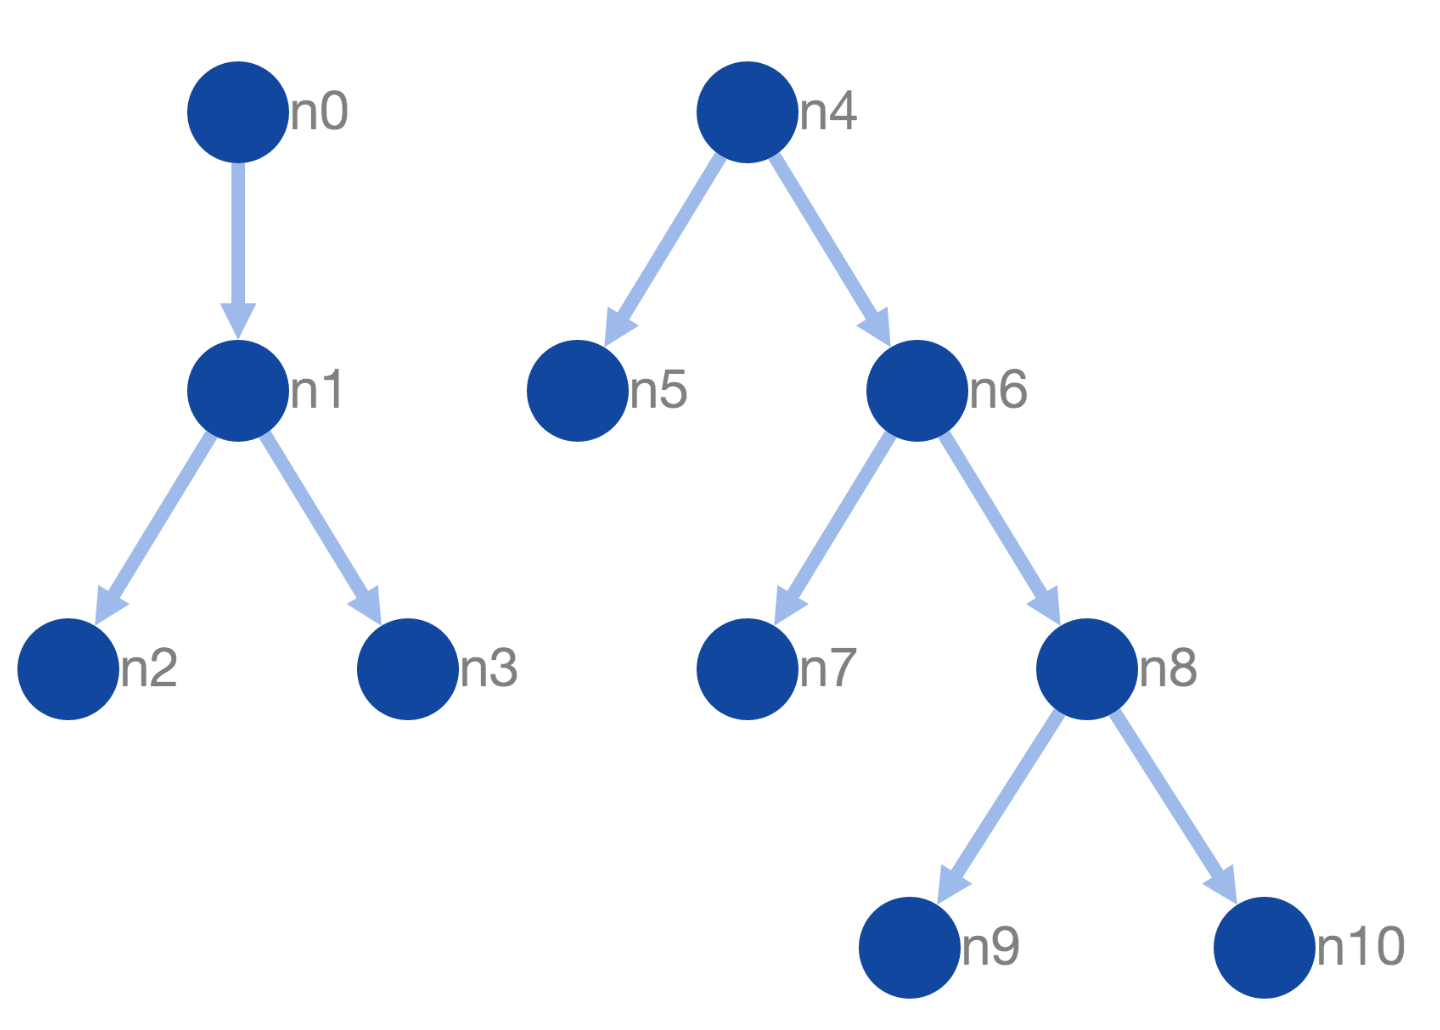
\includegraphics[width=0.4\textwidth]{cytoscape}
\caption{Beispiel Cytoscape}
\label{fig:bsp-cytoscape}
\end{figure}


\begin{longtable}{|p{0.5cm}|p{0.5cm}|p{0.5cm}|p{0.5cm}|p{0.5cm}|p{0.5cm}|p{0.5cm}|p{0.5cm}|p{0.5cm}|p{0.7cm}|p{0.7cm}|}
  \hline
    K1 & K2 & K3 & K4 & K5 & K6 & K7 & K8 & K9 & K10 & K11 \\\hline
    2 & 2 & 2 & 2 & 2 & 2 & 3 & 2 & 2 & 3 & 1\\\hline
    \caption{Bewertung  \textit{cytoscape.js}}
  \label{tab:bewertung-cytoscape}
\end{longtable}

\subsubsection{greuler}
Hier gibt es viele Parallelen zur vorgängigen Bibliothek (\textit{cytoscape.js}). \textit{Greuler} spezialisiert sich nun aber auf die Visualisierung und baut wie viele andere auf \textit{D3}. Bezüglich der Handhabung ist es grösstenteils identisch mit \textit{Cytoscape}, allerdings hat es hier bei weiten nicht so viele Erweiterungsmöglichkeiten. \autoref{fig:bsp-greuler} zeigt ein kleines Beispielnetzwerk. \citep{2_maurizzzio/greuler_2016}

\begin{figure}[htbp]
\centering
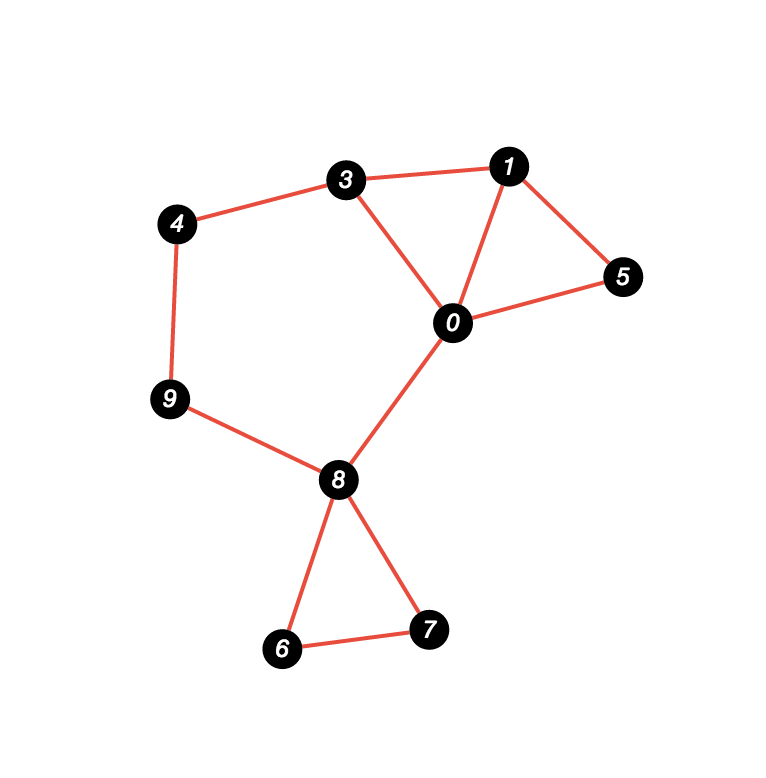
\includegraphics[width=0.4\textwidth]{greuler}
\caption{Beispiel Greuler}
\label{fig:bsp-greuler}
\end{figure}

\begin{longtable}{|p{0.5cm}|p{0.5cm}|p{0.5cm}|p{0.5cm}|p{0.5cm}|p{0.5cm}|p{0.5cm}|p{0.5cm}|p{0.5cm}|p{0.7cm}|p{0.7cm}|}
  \hline
    K1 & K2 & K3 & K4 & K5 & K6 & K7 & K8 & K9 & K10 & K11 \\\hline
    2 & 2 & 2 & 2 & 2 & 4 & 4 & 2 & 2 & 4 & 3\\\hline
    \caption{Bewertung \textit{greuler}}
  \label{tab:bewertung-greuler}
\end{longtable}

\subsubsection{JointJS}
Auch bei JointsJS handelt es sich um eine \textit{open-source}-Bibliothek. Im Gegensatz zu den obigen beiden geht die Funktionalität eine Ebene weiter. Hier werden zusätzlich zur eigentlichen Darstellung auch Werkzeuge zur Manipulation des Diagramms mitgeliefert. Viele Funktionalitäten sind aber erst mit der kostenpflichten Version \textit{Rappid} ver\-füg\-bar, welche auf JointJS aufbaut. \citep{jointsjs}

Die Bibliothek ist für den hier vorliegenden Anwendungsfall zu umfangreich. Die vielen Funktionen machen die Implementation sehr komplex. Dieser Aufwand ist für die eigentlich einfache Anwendung zu gross. Die Vorteile, welche der vorhandene Funktionsumfang bietet, erkennt man erst nach längerer Einarbeitung. Der notwendige Funktionsumfang kann in anderem \gls{Framework}[s] ohne grossen Aufwand selbst implementiert werden. So ist die Übersicht stets geboten und der Code bleibt verhältnismässig einfach.

\begin{longtable}{|p{0.5cm}|p{0.5cm}|p{0.5cm}|p{0.5cm}|p{0.5cm}|p{0.5cm}|p{0.5cm}|p{0.5cm}|p{0.5cm}|p{0.7cm}|p{0.7cm}|}
  \hline
    K1 & K2 & K3 & K4 & K5 & K6 & K7 & K8 & K9 & K10 & K11 \\\hline
    1 & 3 & 3 & 3 & 3 & 4 & 4 & 5 & 4 & 5 & 3\\\hline
    \caption{Bewertung \textit{JointJS}}
  \label{tab:bewertung-jointjs}
\end{longtable}

\subsubsection{jsPlumb}
\label{jsPlumb}

\begin{longtable}{|p{0.5cm}|p{0.5cm}|p{0.5cm}|p{0.5cm}|p{0.5cm}|p{0.5cm}|p{0.5cm}|p{0.5cm}|p{0.5cm}|p{0.7cm}|p{0.7cm}|}
  \hline
    K1 & K2 & K3 & K4 & K5 & K6 & K7 & K8 & K9 & K10 & K11 \\\hline
    2 & 2 & 2 & 1 & 3 & 2 & 2 & 2 & 3 & 3 & 2\\\hline
    \caption{Bewertung \textit{jsPlumb}}
  \label{tab:bewertung-jsplumb}
\end{longtable}

Als einzige Bibliothek basiert jsPlump auf reinen \gls{HTML}-Objekten. Somit werden diese nicht in einem \gls{Canvas} gezeichnet, sondern wie normaler \gls{HTML} Code dargestellt. Somit kann das Aussehen der Elemente direkt durch \gls{CSS}-Klassen angepasst werden. 

\clearpage

Jedoch legt jsPlump den Fokus vor allem auf das Zeichnen und Erstellen von Diagrammen. Es bietet daher eine grosse Anzahl von Funktionen, welche nicht benötigt werden. Zusätzlich müssten benötigte Funktionen zum Teil manuell implementiert werden. Ebenfalls ist nur die limitierte \textit{Community Edition} kostenlos verfügbar. \citep{jsplump}

\begin{figure}
\centering
\begin{subfigure}[b]{0.5\textwidth}
   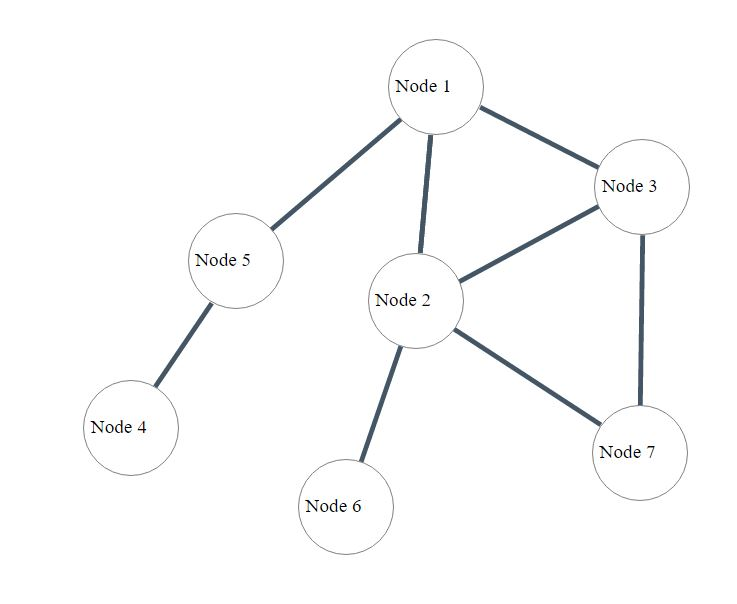
\includegraphics[width=0.9\linewidth]{JsPlump}
\caption{Beispiel JsPlump}
\label{fig:bsp-jsplump}
    \end{subfigure}
\begin{subfigure}[b]{0.4\textwidth}
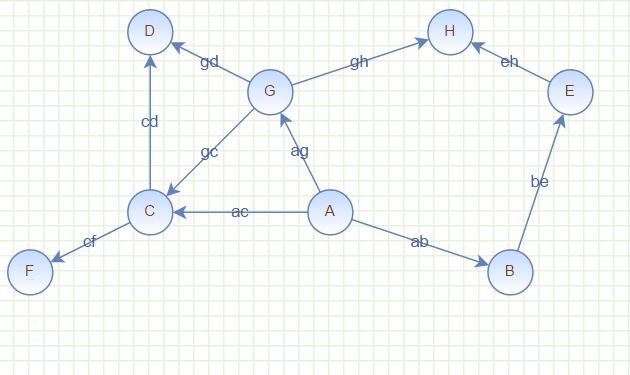
\includegraphics[width=0.9\linewidth]{MxGraphEval}
\caption{Beispiel mxGraph}
\label{fig:bsp-mxgraph}
    \end{subfigure}
    \caption{Frameworks}
\end{figure}



\subsubsection{mxGraph}
Wie auch schon bei der Bibliothek jsPlump setzt mxGraph den Fokus auf die Darstellung und Bearbeitung von ganzen Diagrammen. Es wurde schon als Grundlage von grossen Anwendung wie \textit{draw.io} verwendet. Dadurch ist eine Vielzahl von Funktionen verfügbar. Jedoch würde sich eine Erweiterung dieser eher kompliziert gestalten. \citep{mxGraph}

\begin{longtable}{|p{0.5cm}|p{0.5cm}|p{0.5cm}|p{0.5cm}|p{0.5cm}|p{0.5cm}|p{0.5cm}|p{0.5cm}|p{0.5cm}|p{0.7cm}|p{0.7cm}|}
  \hline
    K1 & K2 & K3 & K4 & K5 & K6 & K7 & K8 & K9 & K10 & K11 \\\hline
    2 & 3 & 3 & 2 & 3 & 2 & 2 & 2 & 4 & 4 & 2\\\hline
    \caption{Bewertung \textit{mxGraph}}
  \label{tab:bewertung-mxgraph}
\end{longtable}


\chapter{Implementation} \label{implementation}

Die Implementation hat zum Ziel, die bereits erarbeitete konzeptionelle Lösung in Form von Code praktisch umzusetzen. Nach einer Übersicht über die abgeschlossene Visualisierung und einem Einblick in die eingesetzten Technologien wird im Detail auf nennenswerte Eigenheiten des Projektes eingegangen.

\section{Übersicht}
Nachfolgend ist die integrierte Visualisierung innerhalb des \gls{ikc-core}[s] ersichtlich (\autoref{fig:overview-implementation}). Sie wurde zwischen der Suche und der Detail-Ansicht platziert. Eine detaillierte Anleitung der Interaktion mit der integrierten Visualisierung ist dem Benutzerhandbuch zu entnehmen. 

\begin{figure}[htbp]
\centerline{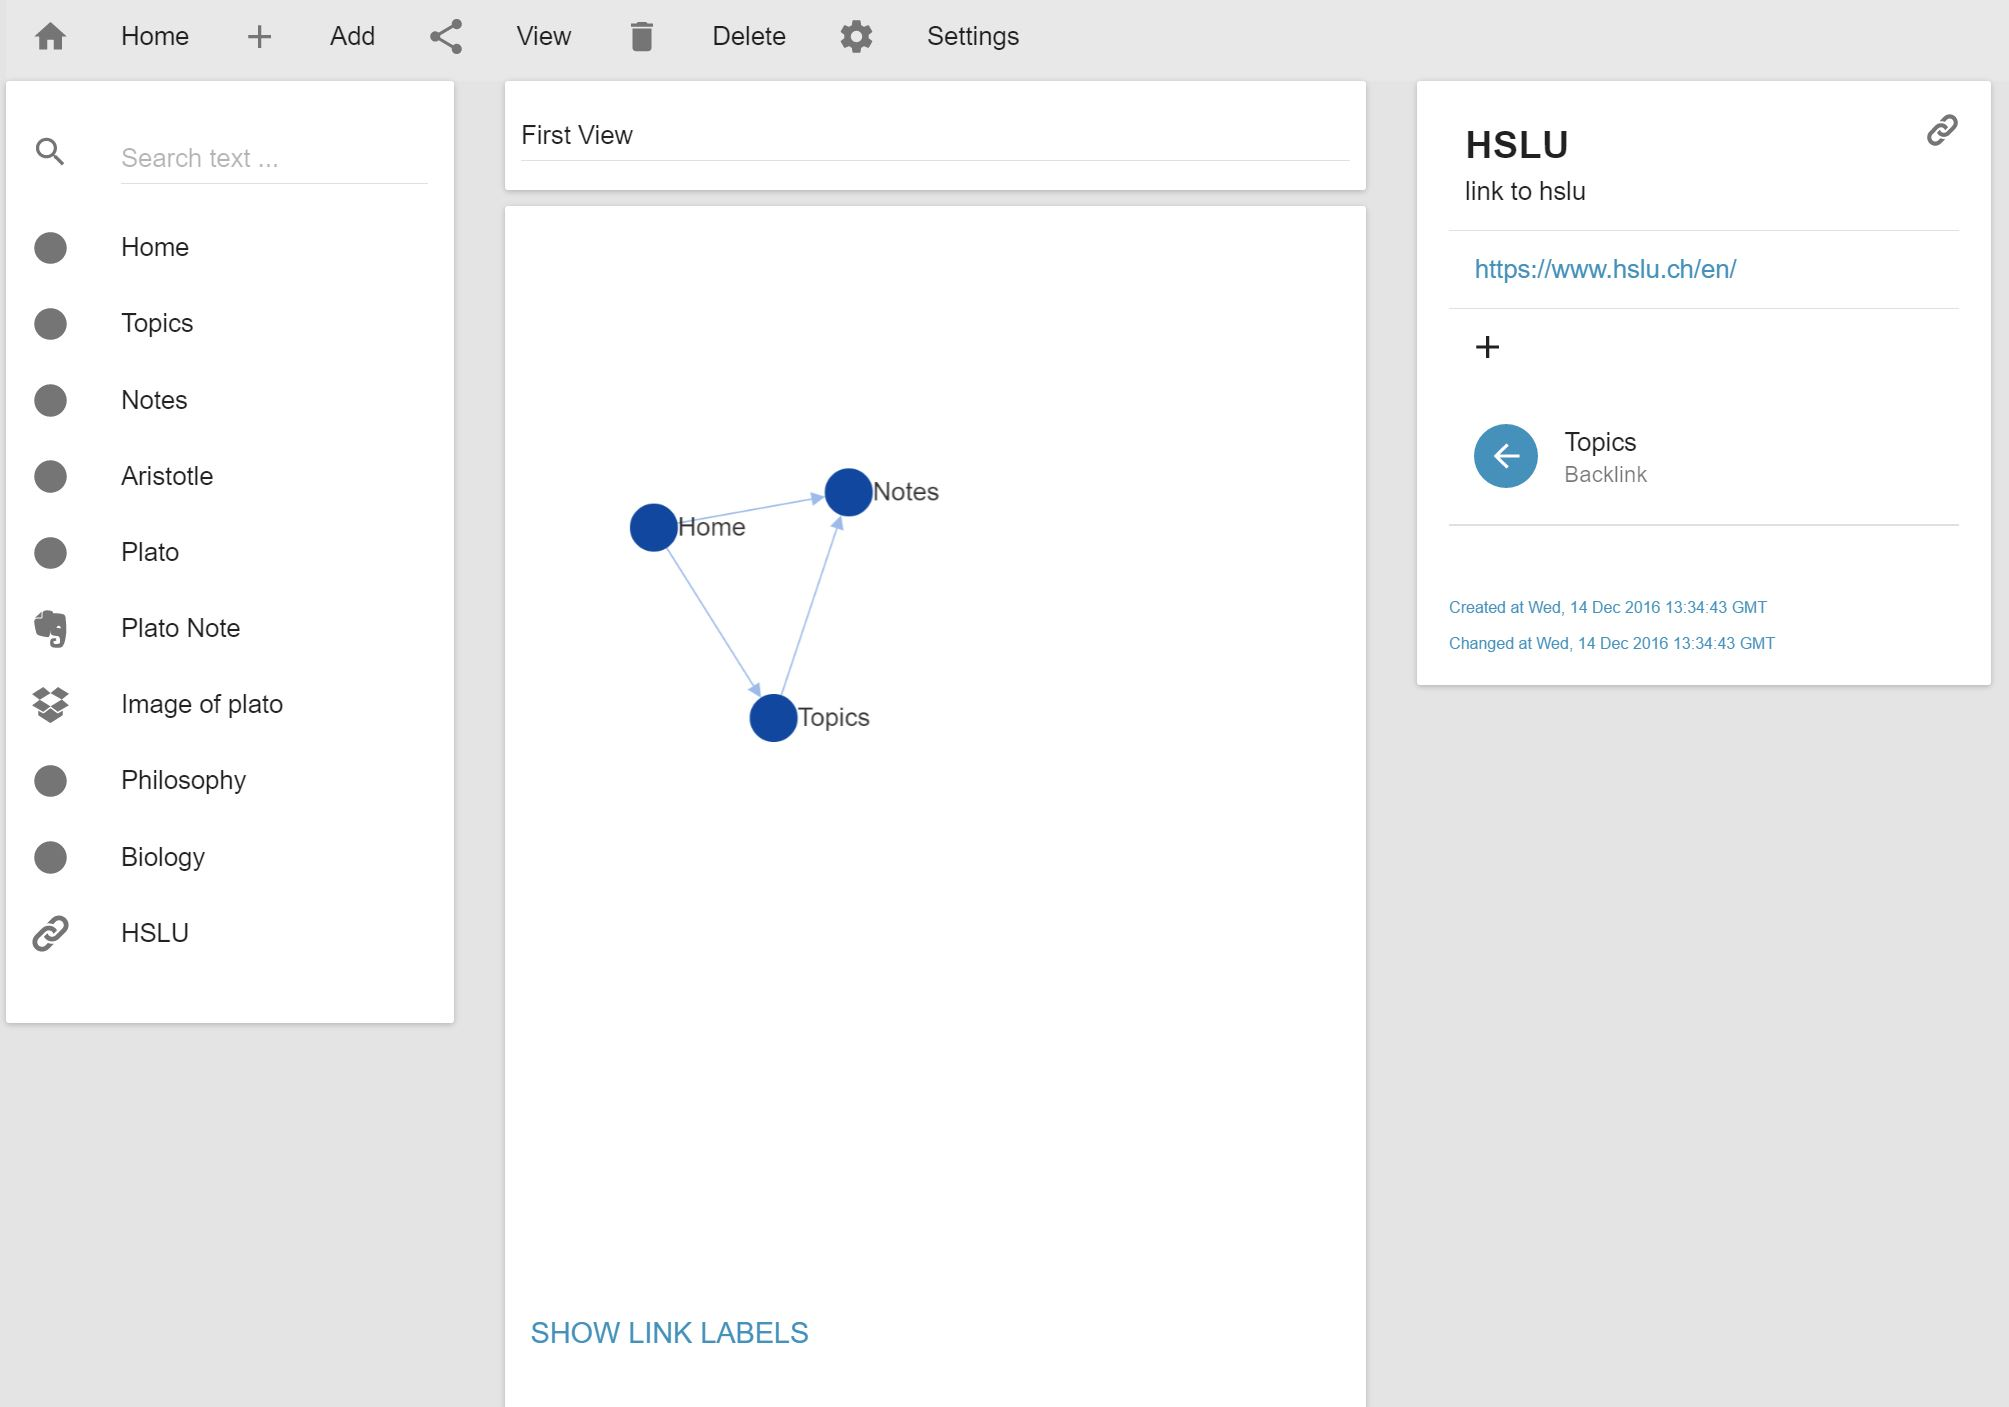
\includegraphics[width=1.3\textwidth]{Overview-Screen}}
\caption {Überblick Implementation}
\label{fig:overview-implementation}
\end{figure}

\section{Technologie} \label{sec:technologie}

Für die Umsetzung wurde aufgrund vieler Parallelen zum \gls{ikc-core} und diverser guten Erfahrungen auf ähnliche Technologien gesetzt. Das Grundgerüst ist daher nahezu identisch mit dem bisherigen. Dabei konnte bereits vorhandenes Wissen wiederverwendet und erweitert werden.

\subsection{Typescript}\label{typescript}

Typescript ist eine von Microsoft entwickelte statisch typisierte Erweiterung von Javascript. Durch die Kompilierung wird es zu üblichen Javascript. Typescript kann bereits während des Schreibens überprüft werden und die Entwicklungstools bieten dadurch viel Hilfestellung. Die Typen sind zwar optional, falls eingesetzt bringen sie aber einige hilfreiche Zusatzfunktionen. Beispielsweise lassen sich Klassen, Interfaces definieren. Dies ist vor allem bei der Entwicklung von grösseren Projekten hilfreich. \citep{typescriptlang}

Typescript wurde vor allem aufgrund der ein\-fach\-er\-en Struk\-tu\-rie\-rung von Projekten und der Typisierung eingesetzt. Zwar kann jegliche Ja\-va\-scri\-pt-Bibliothek eingebunden werden, aber ohne bereits vorhandene statische Typisierung in Form von \textit{Typings} bringt dies keine grossen Vorteile. Unglücklicherweise sind die Typisierungen noch nicht für alle Bibliotheken verfügbar und darum muss teilweise auf eine weniger elegante Integration ausgewichen werden.

\subsection{React}\label{react}

React ist eine Bibliothek für die Entwicklung von Benutzeroberflächen, entwickelt von Facebook. Der Fokus wird insbesondere auf die Interaktivität der Komponenten gelegt, deren Zustände ständig wechseln können. Bei Zustandsänderungen aktualisiert React automatisch alle notwendigen Komponenten. Die Komponentenbauweise bringt hohe Modularität und Wiederverwendbarkeit mit sich, untereinander sind die Komponenten entkoppelt. Einmal erstellte Komponenten können an beliebigen Stellen wiederverwendet werden, so zum Beispiel ein Suchfeld. Verwendet werden dies Komponenten immer in der \textit{XML}-Syntax. Grundsätzlich wird eine React-Komponente in verschiedene Teile zerlegt (\autoref{listing:react-component}): 

\begin{enumerate}
    \item \label{props} \textit{Props-Schnittstelle} - definiert, mit welchen Parameter eine Komponente benutzt werden muss. Optionale Parameter werden mit einem Fragezeichen (\texttt{\textbf{?}}) gekennzeichnet. Innerhalb der Komponente kann \texttt{this.props} auf die Eigenschaften zugreifen. Jedoch können keine Werte aktualisiert werden.
    \item \label{states} \textit{State-Schnittstelle} - spezifiziert den Zustand der Komponente. Diese kann sich abhängig von Ereignissen innerhalb der Komponente aktualisieren. Mit \texttt{this.state} kann ein Zugriff stattfinden.
    \item \textit{Implementierung} - jede Komponente implementiert die Schnittstelle \textit{React.Component$<>$}. Einzig die Methode \texttt{render} muss implementiert werden. Darin wird der darzustellende Inhalt aus \gls{HTML}-Elementen oder weiteren React-Komponenten zusammengestellt. 
    \item \textit{Verwendung} - nach der Implementierung kann jede Komponente von anderen React-Komponenten innerhalb deren \texttt{render} Methode verwendet werden.
\end{enumerate}

\begin{listing}[htbp]
\inputminted[
frame=lines,
framesep=2mm,
baselinestretch=1.2,
linenos,
breaklines=true
]{js}{sourcecode/common/react.ts}
\caption{Beispiel React Komponente}
\label{listing:react-component}
\end{listing}

Jede React-Komponente durchläuft grundlegende Zustände. An diesen kann mit sogenannten \textit{Lifecycle}-Methoden in den jeweiligen Prozess eingegriffen werden. Bei der Implementierung der Visualisierung wurden hauptsächlich folgenden Methoden eingesetzt.
%Zusätzlich durchläuft jede React-Komponente drei grundlegende Zustände, in welchen mit verschiedenen speziellen Methode darauf reagiert werden kann:

\begin{itemize}
   \item \textit{Mounting} - hier werden verschiedene Methoden abgearbeitet, bis eine Komponente erstellt und zu einem \gls{HTML}-Element konvertiert wird.
   \begin{enumerate}
     \item \texttt{constructor}
     \item \texttt{componentWillMount}
     \item \texttt{render}
     \item \texttt{componentDidMount}
   \end{enumerate}
   \item \textit{Updating} - ein Update kann entweder durch eine Aktualisierung des \textit{State} oder der \textit{Props} erfolgen.
   \begin{enumerate}
     \item \texttt{componentWillReceiveProps}
     \item \texttt{shouldComponentUpdate}
     \item \texttt{componentWillUpdate}
     \item \texttt{render}
     \item \texttt{componentDidUpdate}
   \end{enumerate}
   \item \textit{Unmounting} - dieser Schritt wird ausgeführt, bevor die Komponente entfernt wird.
   \begin{enumerate}
     \item \texttt{componentWillUnmount}
   \end{enumerate}
\end{itemize}

Ein weiterer, besonderer Punkt von React ist der uni\-di\-rek\-tio\-nale Datenfluss. Dieser wird nachfolgend im \autoref{unidirectional} behandelt. \citep{reactjs, reactjs-blog}

\subsection[Datenfluss]{Unidirektionaler Datenfluss}\label{unidirectional}
Die Verwendung von unidirektionalen Datenflüssen erleichtert die Verwendung von React-Komponenten, welche auch in dem, von Facebook präsentierten, Architektur-Muster \textit{Flux} enthalten sind. Auf eine strikte Verwendung von \textit{Flux} wurde verzichtet, jedoch wurden trotzdem unidirektionale Datenflüsse eingesetzt. Wie diese genau funktionieren, wird anhand des Beispiels in \autoref{fig:unidirectional} genauer aufgezeigt: 
   \begin{enumerate}
     \item Die \textit{GraphScreen}-Komponente verwendet die \textit{Graph}-Komponente in ihrer \texttt{render}-Methode in Form von (\texttt{<Graph ... />}). 
     \item Sobald den \textit{Graph}-Komponente erstellt ist, wird der Zustand anhand der übergebenen Parameter initialisiert.
     \item Angestossen von \gls{Event}s aus dem \textit{cytoscape}-Framework werden \gls{Callback}-Methoden aufgerufen, um Information an die \textit{GraphScreen}-Komponente zu senden. Die entsprechenden Methoden werden als Parameter an die \textit{Graph}-Komponente übergeben, beispielsweise \texttt{this.prop.handleNewLink(...)}
     \item Innerhalb den von der \textit{Graph}-Komponente aufgerufenen Methoden in der \textit{GraphScreen}-Komponente wird nun der Zustand der \textit{GraphScreen}-Komponente aktualisiert. Dies geschieht mit der Methode \texttt{this.setState({...})}, welche von dem React-Framework zur Verfügung gestellt wird. Hier werden die Änderungen weitergegeben. Diese werden im Hintergrund ausgeführt.
     \item Sobald der Zustand angepasst wurde, wird die \texttt{render}-Methode neu ausgeführt. Dadurch werden die Aktualisierungen der \textit{Graph}-Komponente per Parameter (\textit{Props}) weitergegeben.
     \item Durch die Aktualisierung der Parameter wird nun auch die \texttt{render} Methode der \textit{Graph}-Komponente neu ausgeführt und der Zustand aktualisiert. 
   \end{enumerate}

\begin{figure}[htbp]
\centerline{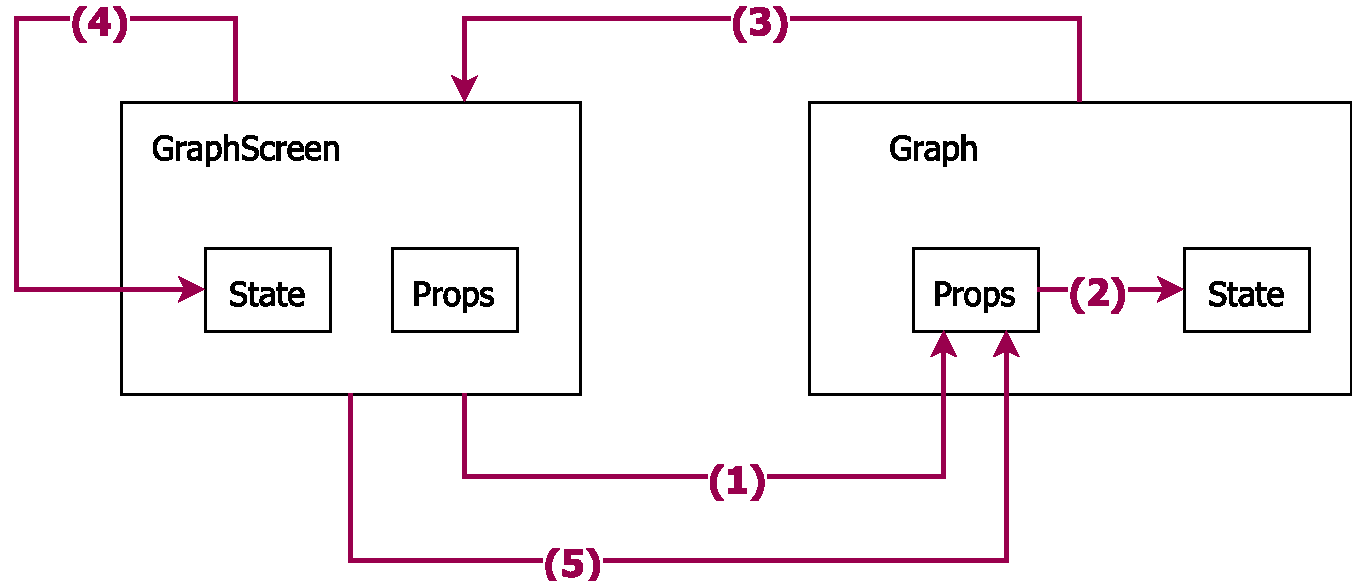
\includegraphics[width=1\textwidth]{unidirectional}}
\caption {Unidirektionaler Datenfluss}
\label{fig:unidirectional}
\end{figure}


\subsection{Material Design}

Die React Erweiterung \textit{Material UI} ist zuständig für das Erscheinungsbild der Visualisierung, wie auch schon beim \textit{ikc-core}. Dafür gibt es diverse vorgefertigte Komponenten, welche praktisch ohne Zusatzaufwand verwendet werden können. Googles Material Design kombiniert klassische Design Prinzipien mit Innovation auf Technik und Wissenschaft. \citep{react-material-ui, google-material-ui}

\subsection{Webpack}

Mit der Verwendung von zahlreichen Erweiterungen und \hyperref[typescript]{\textit{Typescript}} als primäre Programmiersprache ergeben sich diverse Abhängigkeiten und auch eine Kompilierung ist notwendig. Für die Sammlung der Abhängigkeiten und die Übersetzung in Javascript wird Webpack eingesetzt. Das Resultat ist beispielweise eine Javascript-Datei, welche alle Abhängigkeiten im richtigen Format enthält. Darum ist vom Webserver nur eine Datei zu laden, so verkürzt die Ladezeit zusätzlich. \citep{webpack}

\section[Interkation]{Interaktion mit bestehenden Komponenten}\label{interaktion}

Innerhalb der Visualisierung werden verschiedene bestehende Komponenten aus dem \gls{ikc-core} genutzt. Diese implementieren die beschriebenen Schnittstellen (\autoref{schnittstellen}) und werden an den \textit{GraphScreen} üb\-er\-ge\-ben. Die Implementationen gelten als Voraussetzung für die Verwendung der Visualisierung.

\subsubsection{GraphDialogFactory/GraphSearchFieldFactory}
Mit Hilfe dieser beiden Klassen kann die Visualisierung auf \hyperref[react]{\textit{React}}-Komponenten zugreifen, welche im \gls{ikc-core} implementiert sind. Diese sind in erster Linie Dialoge oder Suchfelder. Im folgenden Ablaufdiagramm (\autoref{fig:interaction-dialog} und \autoref{listing:interaction-factory}) ist die Funktionsweise am Beispiel des \textit{NewNodeDialog}s detailliert ersichtlich. Das Prinzip gilt ebenfalls für die Dialoge \textit{NewNodeToConnect}, \textit{NodeSearchToConnect} und die beiden Suchfelder \textit{NodeSearchField} und \textit{LinkSearchField}:

\begin{enumerate}
    \item Die Komponente \textit{GraphVisualisation} erstellt ein Objekt der Klasse \textit{GraphDialogFactory}. Sie implementiert die Schnittstelle \hyperref[DialogFactory]{\textit{DialogFactory}} aus der Visualisierung.
    \item Bei der Verwendung der Visualisierung (\textit{GraphScreen}) wird unter anderem das \textit{GraphDialogFactory}-Objekt an die Visualisierung übergeben. Dabei ändert das Objekt den Typ von \textit{GraphDialogFactory} zu \hyperref[DialogFactory]{\textit{DialogFactory}}. Da ersteres der Visualisierung unbekannt ist, kann so eine beidseitige Kopplung verhindert werden. Alle Objekte, welche übergeben werden, sind in der Schnittstelle \hyperref[GraphScreenProps]{\textit{GraphScreenProps}} zusammengefasst. Diese wird innerhalb des \hyperref[react]{\textit{React}}-Frameworks implementiert.
    \item Wenn nun die Visualisierung einen \textit{NewNode}-Dialog benötigt, wird dieser von der \textit{GraphDialogFactory} bezogen. Diese wird von dem \hyperref[GraphScreenProps]{\textit{GraphScreenProps}} zur Verfügung gestellt. Dazu wird die Methode \texttt{getNewNodeDialog} aufgerufen, welcher die benötigten Informationen für die Erstellung des Dialogs mitgegeben werden.
    \item Nachdem der Dialog geschlossen wurde, werden die entsprechenden \gls{Callback}-Methoden ausgeführt. Diese stehen dem Dialog durch das \textit{DialogNewNodeProps}-Objekt zu Verfügung, welches zuvor von der \textit{GraphDialogFactory} anhand der Informationen der Visualisierung entsprechend bestückt wurde. Somit wird die Visualisierung über das Resultat des Dialogs informiert und kann die Informationen entsprechend weiterverarbeiten. 
\end{enumerate}

\begin{figure}[htbp]
\centerline{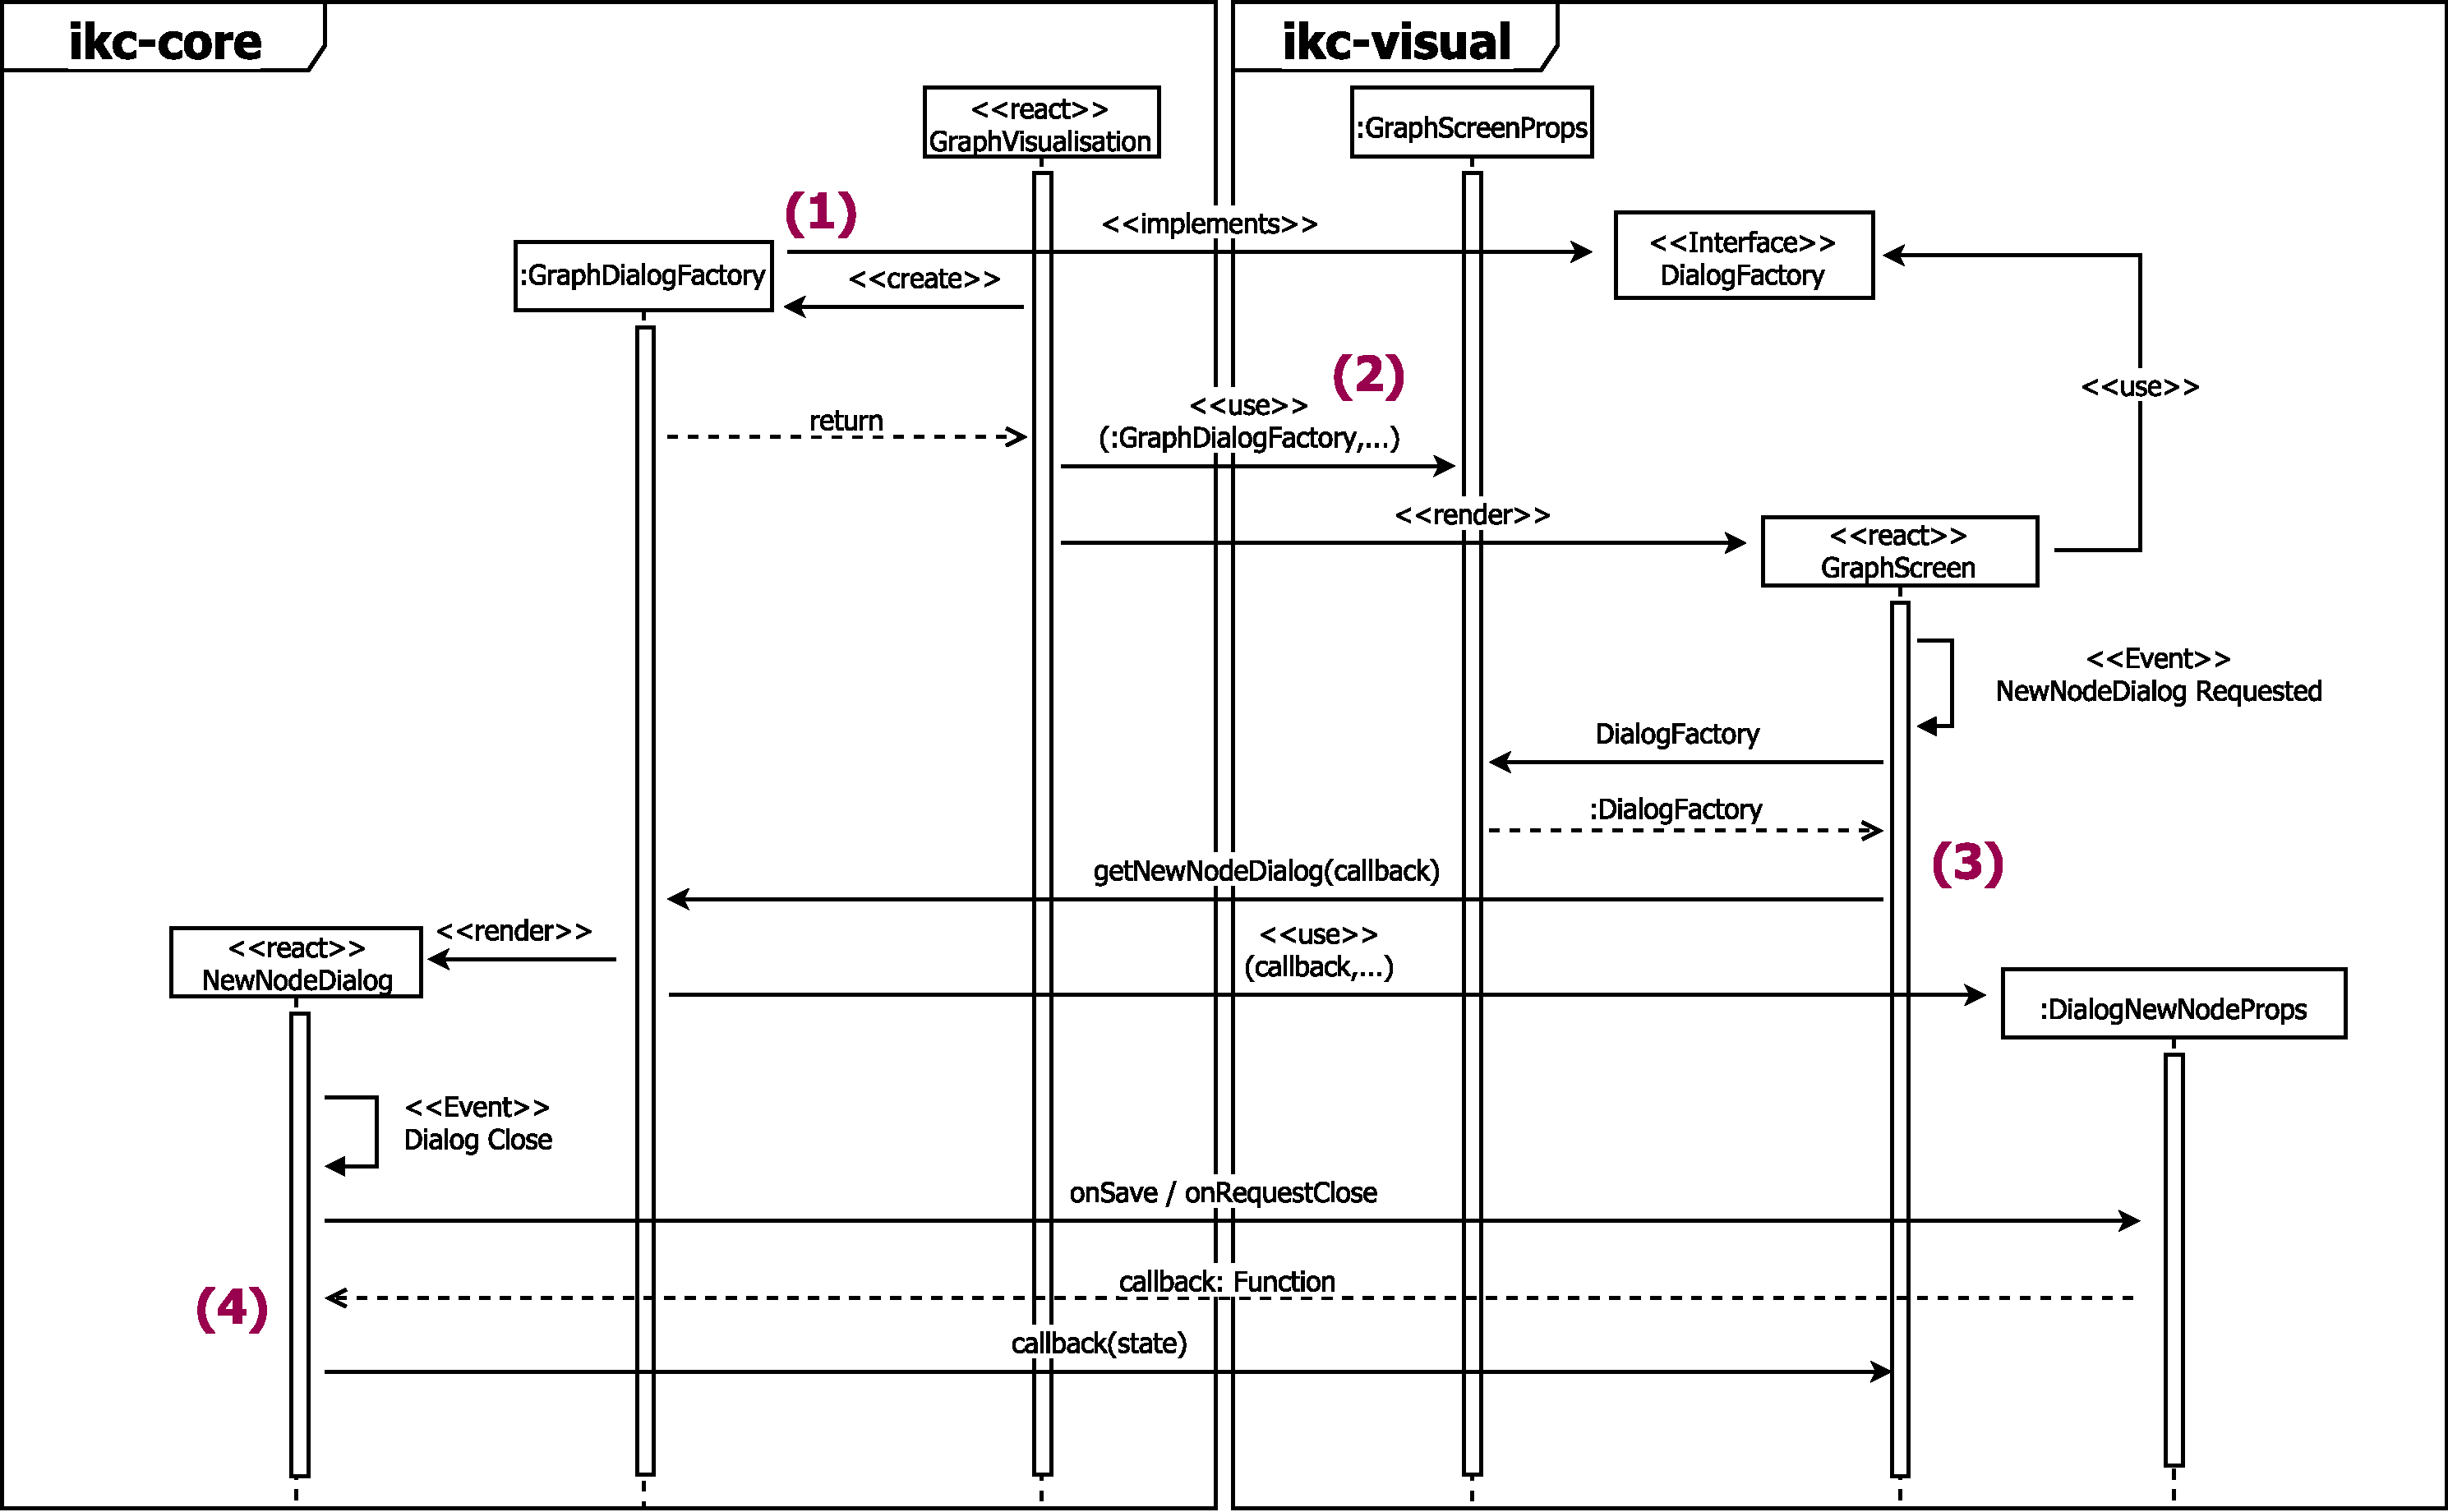
\includegraphics[width=1.3\textwidth]{ExternalComponentDialog}}
\caption{Interaktion mit den Factories}
\label{fig:interaction-dialog}
\end{figure}

\begin{listing}[htbp]
\inputminted[
frame=lines,
framesep=2mm,
baselinestretch=1.2,
linenos,
breaklines=true
]{js}{sourcecode/common/InteractionFactory.ts}
\caption{Beispiel Interaktion Factory}
\label{listing:interaction-factory}
\end{listing}

\subsubsection{Weitere Implementationen}
Mit Hilfe der Implantation der Schnittstellen \hyperref[NodeInformationProvider]{\textit{NodeInformationProvider}},  \hyperref[OperationService]\textit{OperationService},  \hyperref[IdentityService]{\textit{IdentityService}} können der Visualisierung konkrete Implementationen zu Verfügung gestellt werden (\autoref{fig:interaction-nodeinformationprovider}, \autoref{fig:interaction-identityservice}, \autoref{fig:interaction-operationservice} und \autoref{listing:interaction-components}):
\begin{enumerate}
    \item Das entsprechende Objekt der Implementierung wird erstellt.
    \item Bei der Erstellung der Visualisierung wird das Objekt übergeben.
    \item Über \hyperref[GraphScreenProps]{\textit{GraphScreenProps}} kann die Visualisierung auf das entsprechende Objekt zugreifen und mit den Methoden die benötigten Informationen abrufen.
\end{enumerate}

\begin{figure}[htbp]
\centerline{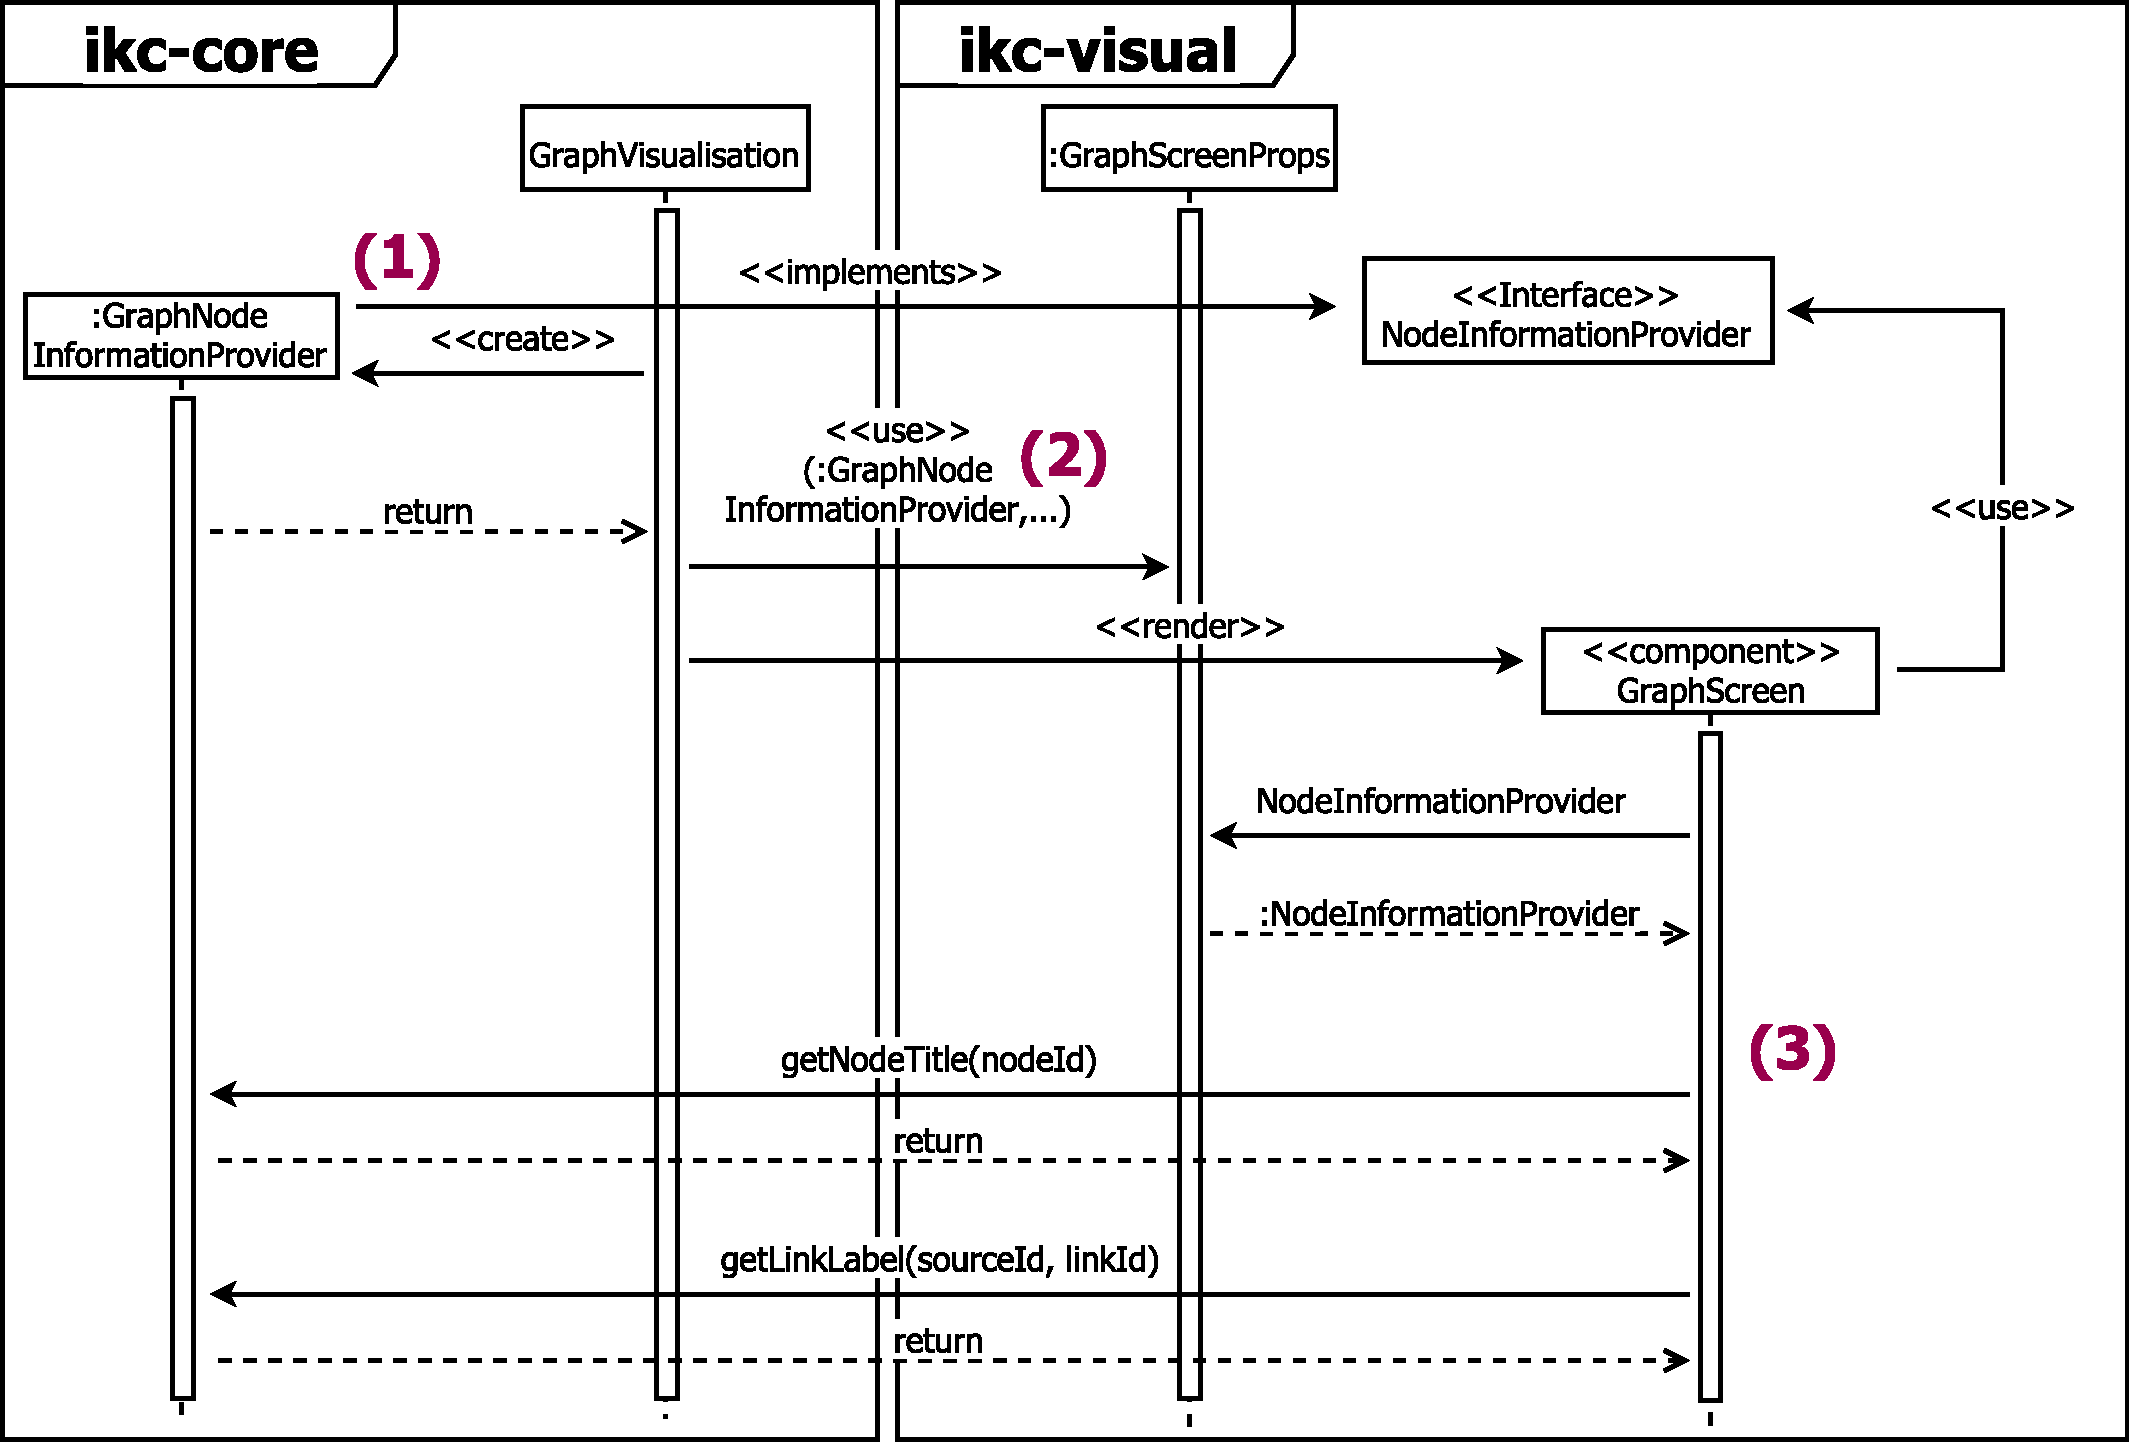
\includegraphics[width=1.3\textwidth]{ExternalComponentInformationProvider}}
\caption{Interaktion mit dem NodeInformationProvider}
\label{fig:interaction-nodeinformationprovider}
\end{figure}


\begin{figure}[htbp]
\centerline{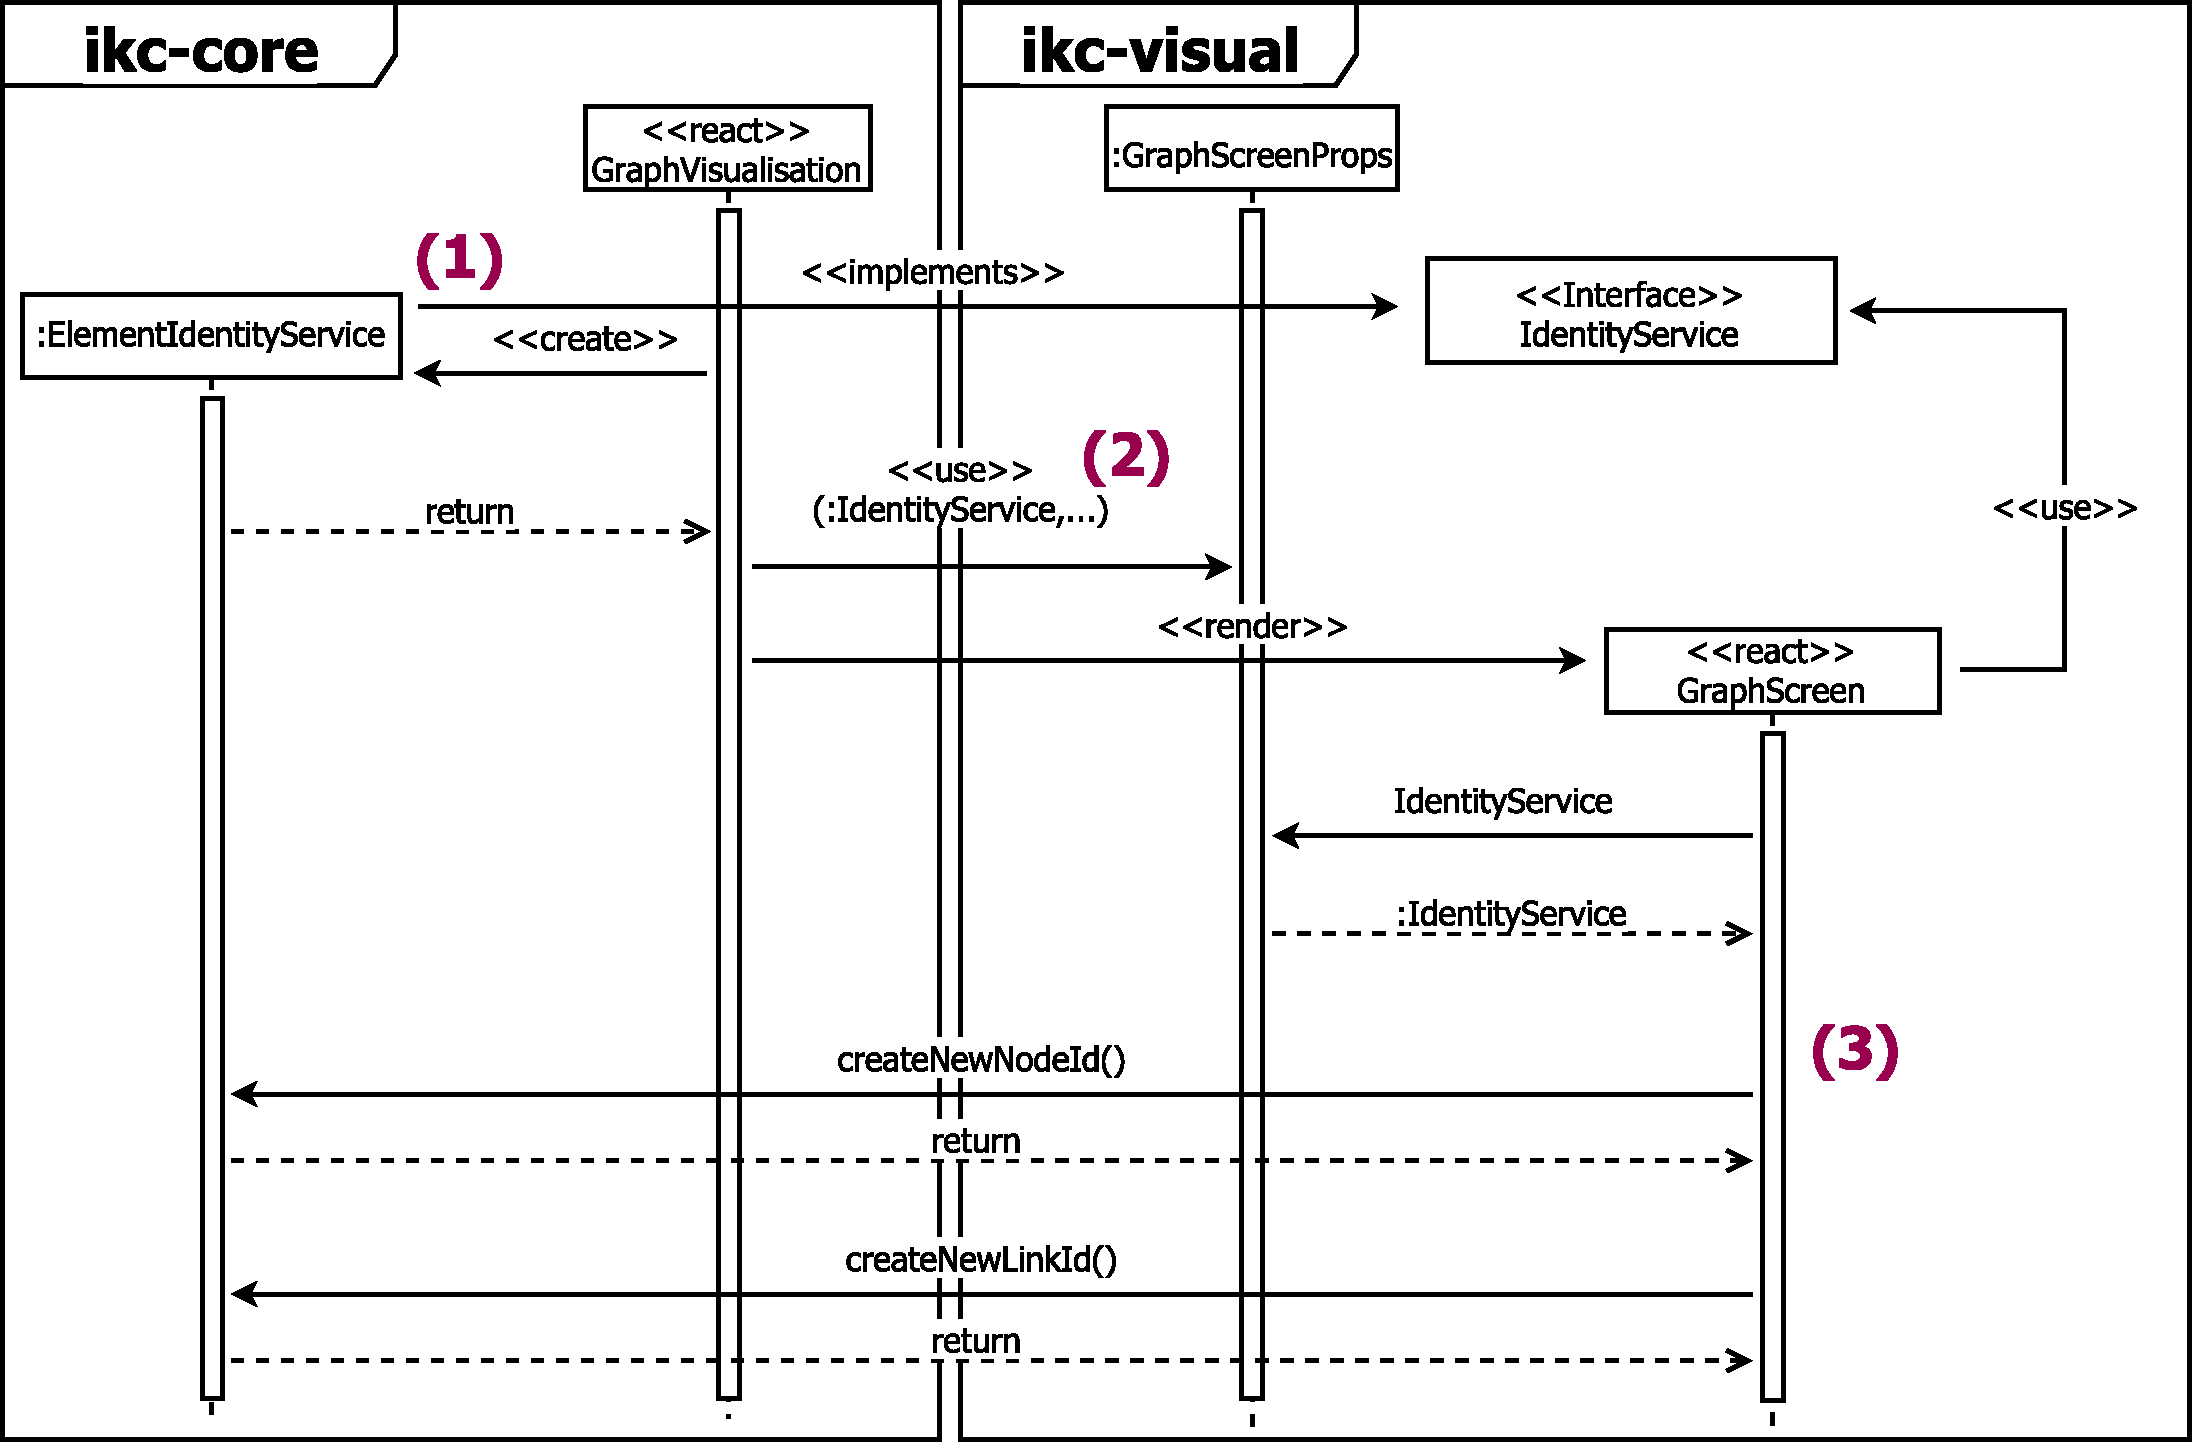
\includegraphics[width=1.3\textwidth]{ExternalComponentIdentityService}}
\caption{Interaktion mit dem IdentityService}
\label{fig:interaction-identityservice}
\end{figure}


\begin{figure}[htbp]
\centerline{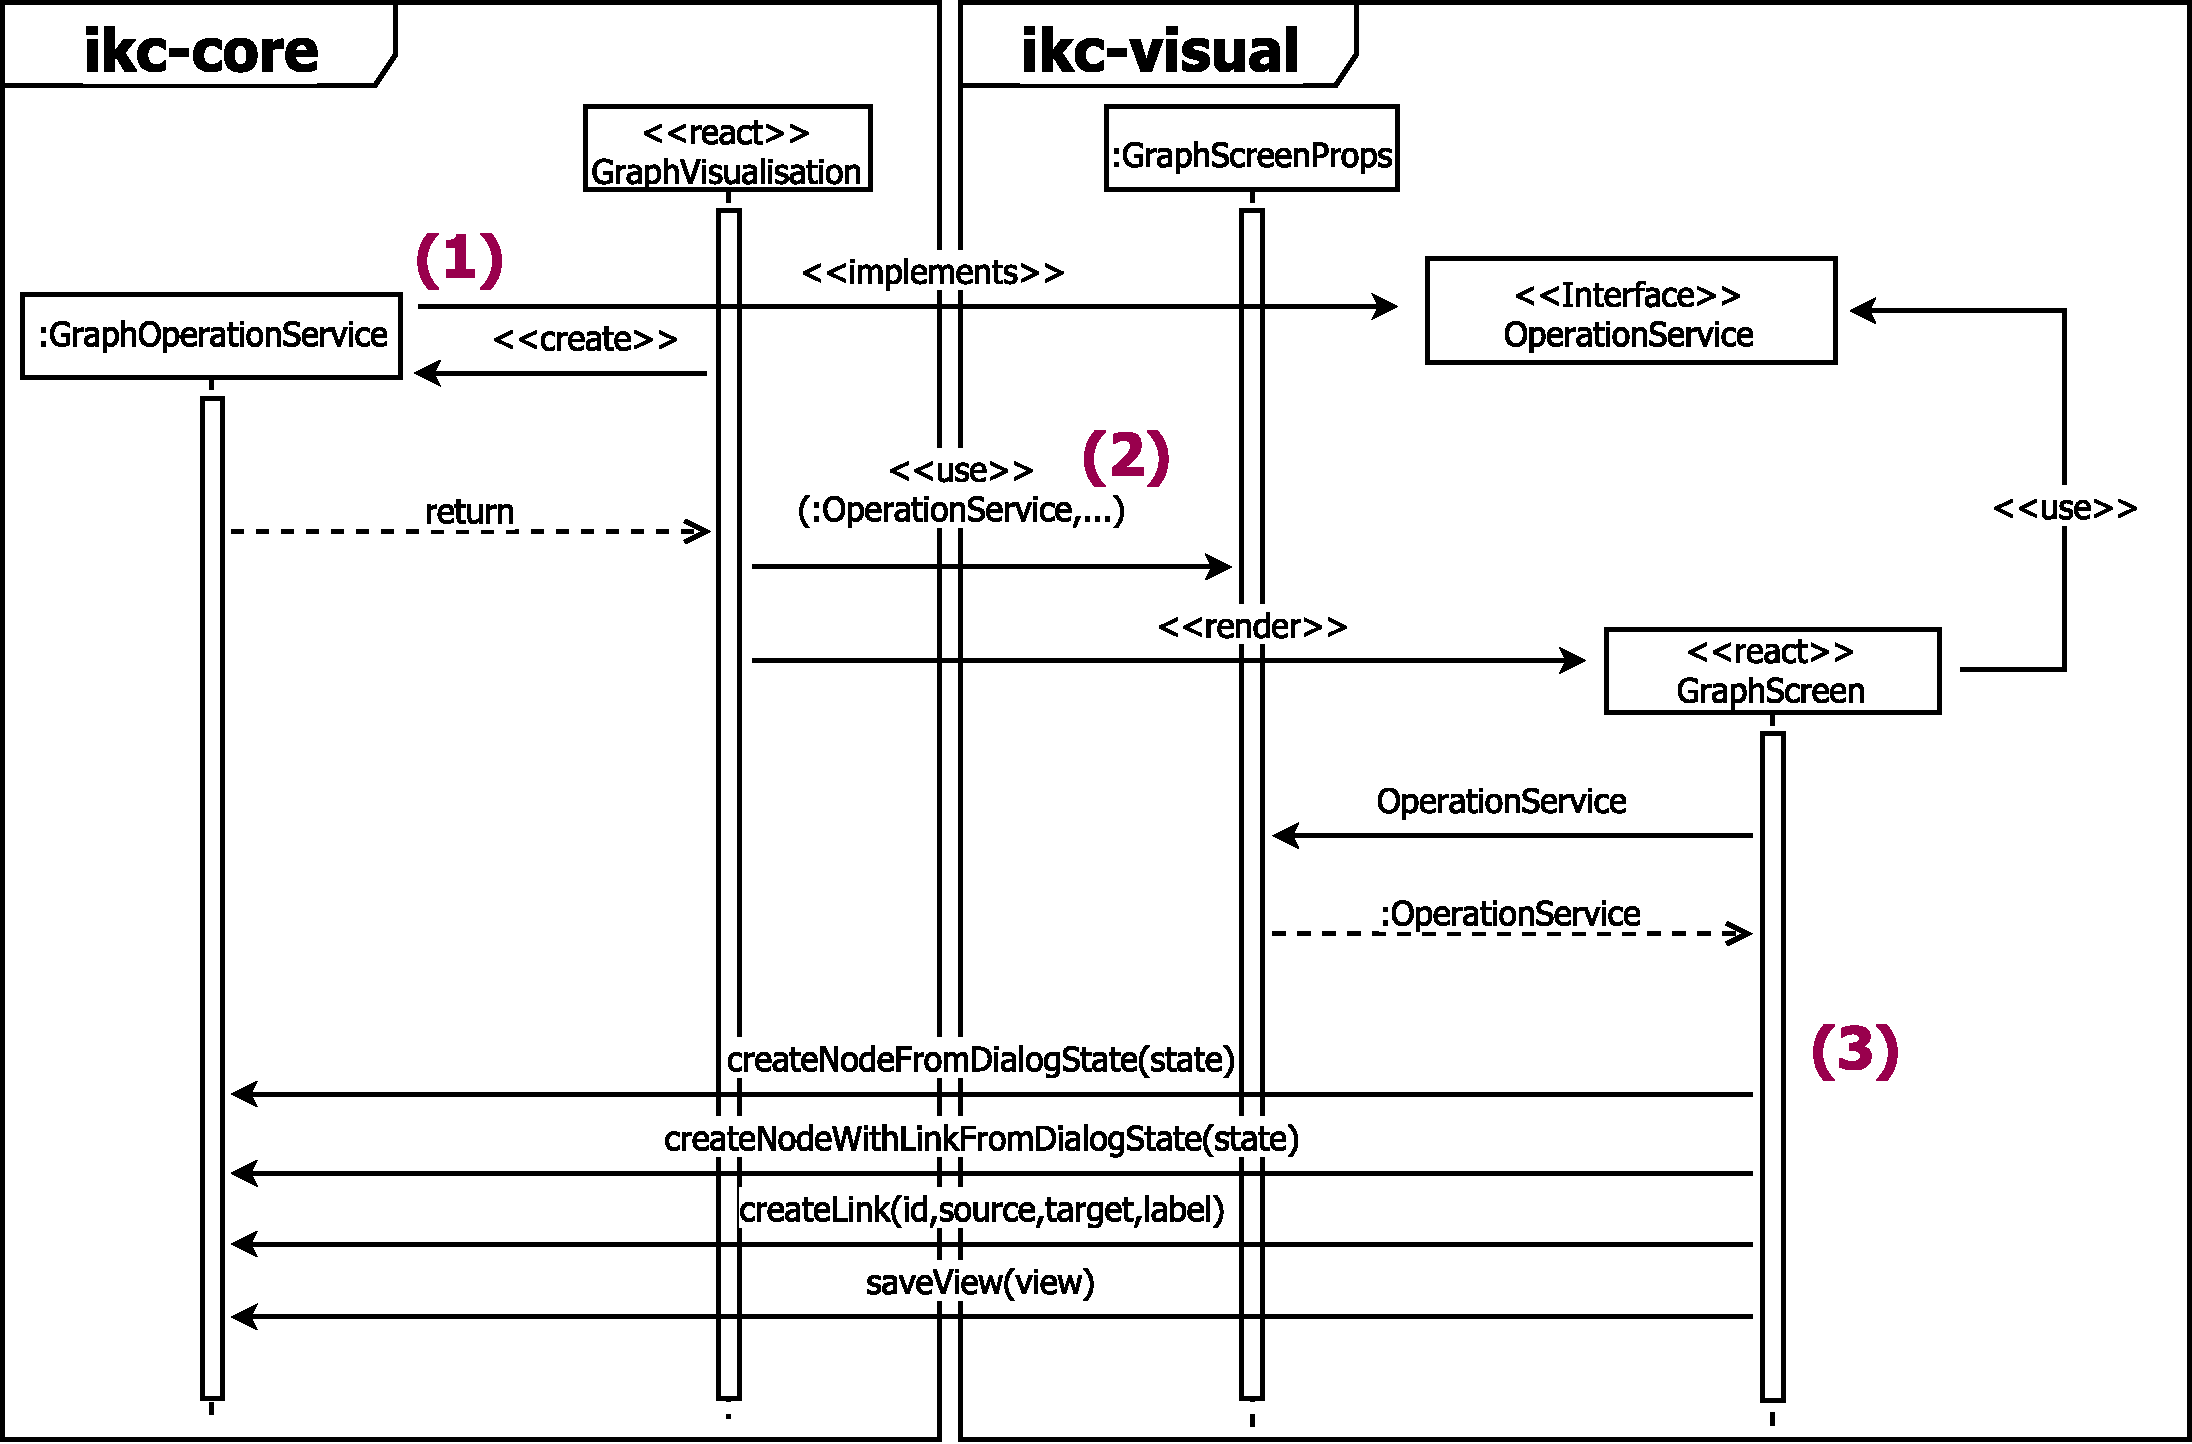
\includegraphics[width=1.3\textwidth]{ExternalComponentOperationService}}
\caption{Interaktion mit dem OperationService}
\label{fig:interaction-operationservice}
\end{figure}

\begin{listing}[htbp]
\inputminted[
frame=lines,
framesep=2mm,
baselinestretch=1.2,
linenos,
breaklines=true
]{js}{sourcecode/common/InteractionComponents.ts}
\caption{Beispiel: Interaktion weiterer Komponenten}
\label{listing:interaction-components}
\end{listing}

\section{Drag'n'Drop}
\label{dnd}
Die \gls{Drag'n'Drop}-Funktionalität bietet sowohl auf dem mobilen als auch auf dem Desktop-Gerät die Möglichkeit, Benutzerinteraktion intuitiv und einfach zu gestalten. Wie im \autoref{subsec:aktionen} bereits definiert, sind dies \textit{Add Node}, \textit{New Link}, \textit{Link To Existing Node} und \textit{Update Position}. Dies kann sowohl innerhalb der Visualisierung oder auch von einer externen Komponente aus geschehen. In diesem Abschnitt werden die grundsätzlichen Abläufe erläutert, welche es ermöglichen einen \gls{Node} von einer externen Komponente in die Visualisierung zu ziehen. Wie die Aktionen innerhalb der Visualisierung funktionieren, wird im \autoref{subsec:graph-manipulation} erläutert.

Grundsätzlich wird der Vorgang des \gls{Drag'n'Drop}[s] in vier Phasen unterteilt:

\begin{itemize}
    \item \textit{Registration} - Alle Elemente, auf welche ein Drag (Nodes) oder ein Drop (Visualisierung) möglich sein soll, müssen registriert werden. 
    \item \textit{Drag} - Ein Drag wird mit einem Klick oder Tap auf einem Element gestartet.
    \item \textit{Move} - Das Element wird auf dem Monitor bewegt.
    \item \textit{Drop} - Das Element wird auf der Visualisierung losgelassen. Wenn dies an einer freien Stelle geschieht, wird der \gls{Node} an dieser Stelle hinzugefügt (4.a). Geschieht dies jedoch über einem bestehenden \gls{Node}, wird ein neuer \gls{Link} erstellt und der neue \gls{Node} im Umkreis des bestehenden positioniert (4.b).
\end{itemize}


\begin{figure}[htbp]
\centerline{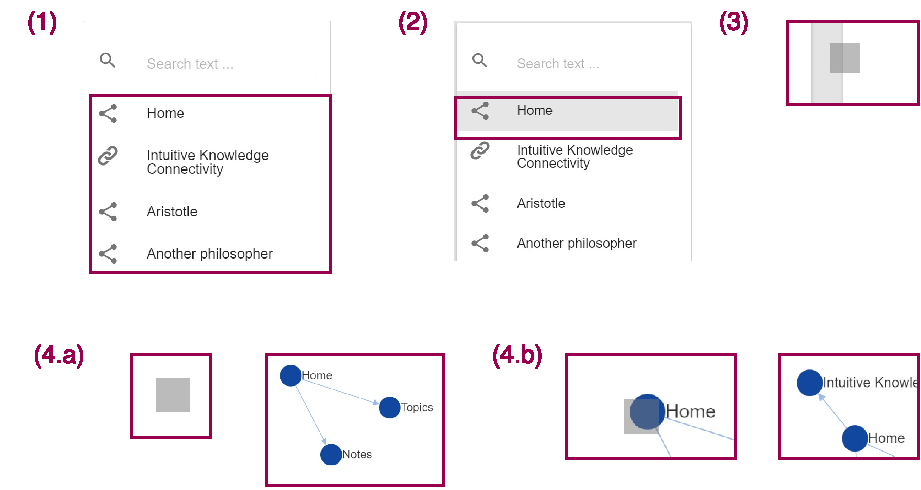
\includegraphics[width=1.3\textwidth]{DragNDropScreen}}
\caption{Übersicht \gls{Drag'n'Drop}}
\label{fig:dnd-screen}
\end{figure}

Damit diese Phasen korrekt ausgeführt werden können, ist es wichtig zu wissen, welcher \gls{Node} an der Aktion beteiligt ist. Weiter müssen verschiedene \gls{Event}s abgefangen und verarbeitet werden. Um dies möglichst simpel und effizient zu implementieren, wird dies in eine externe \gls{Javascript}-Datei ausgelagert und somit vom Rest entkoppelt (\autoref{listing:dnd-handling}). Dieses bietet zwei zwingende und zwei optionale Methoden:
\begin{itemize}
    \item \textit{registerDragZone} - Mit der Registration wird das \gls{Drag'n'Drop} auf dem entsprechenden \gls{HTML}-Element aktiviert. Dazu muss das entsprechende \gls{HTML}-Objekt als auch die entsprechende Node-ID übergeben werden.
    \item \textit{registerDropZone} - Ebenfalls muss die Visualisierung als Drop-Zone registriert werden. Dadurch kann bei einem Drop über ihr die \gls{Callback}-Methode \textit{onDrop} ausgeführt werden, welche übergeben werden muss. 
    \item \textit{registerCallbackForStart} - Hiermit wird jedem Element ermöglicht, bei einem Start eines \gls{Drag'n'Drop} informiert zu werden. 
    \item \textit{registerCallbackForEnd} - Dadurch ist es möglich benachrichtigt zu werden, sobald der \gls{Drag'n'Drop}-Vorgang beendet ist.
\end{itemize}

\begin{listing}[htbp]
\inputminted[
frame=lines,
framesep=2mm,
baselinestretch=1.2,
linenos,
breaklines=true
]{js}{sourcecode/common/MobileDrop.js}
\caption{Drag'n'Drop Handhabung}
\label{listing:dnd-handling}
\end{listing}

Wie diese Phasen im Detail abgehandelt wird, ist in Ablaufdiagramm (\autoref{fig:dnd-sequence}) ersichtlich. Sie sind ebenfalls in die vier Phasen des \gls{Drag'n'Drop} unterteilt.

\begin{figure}[htbp]
\centerline{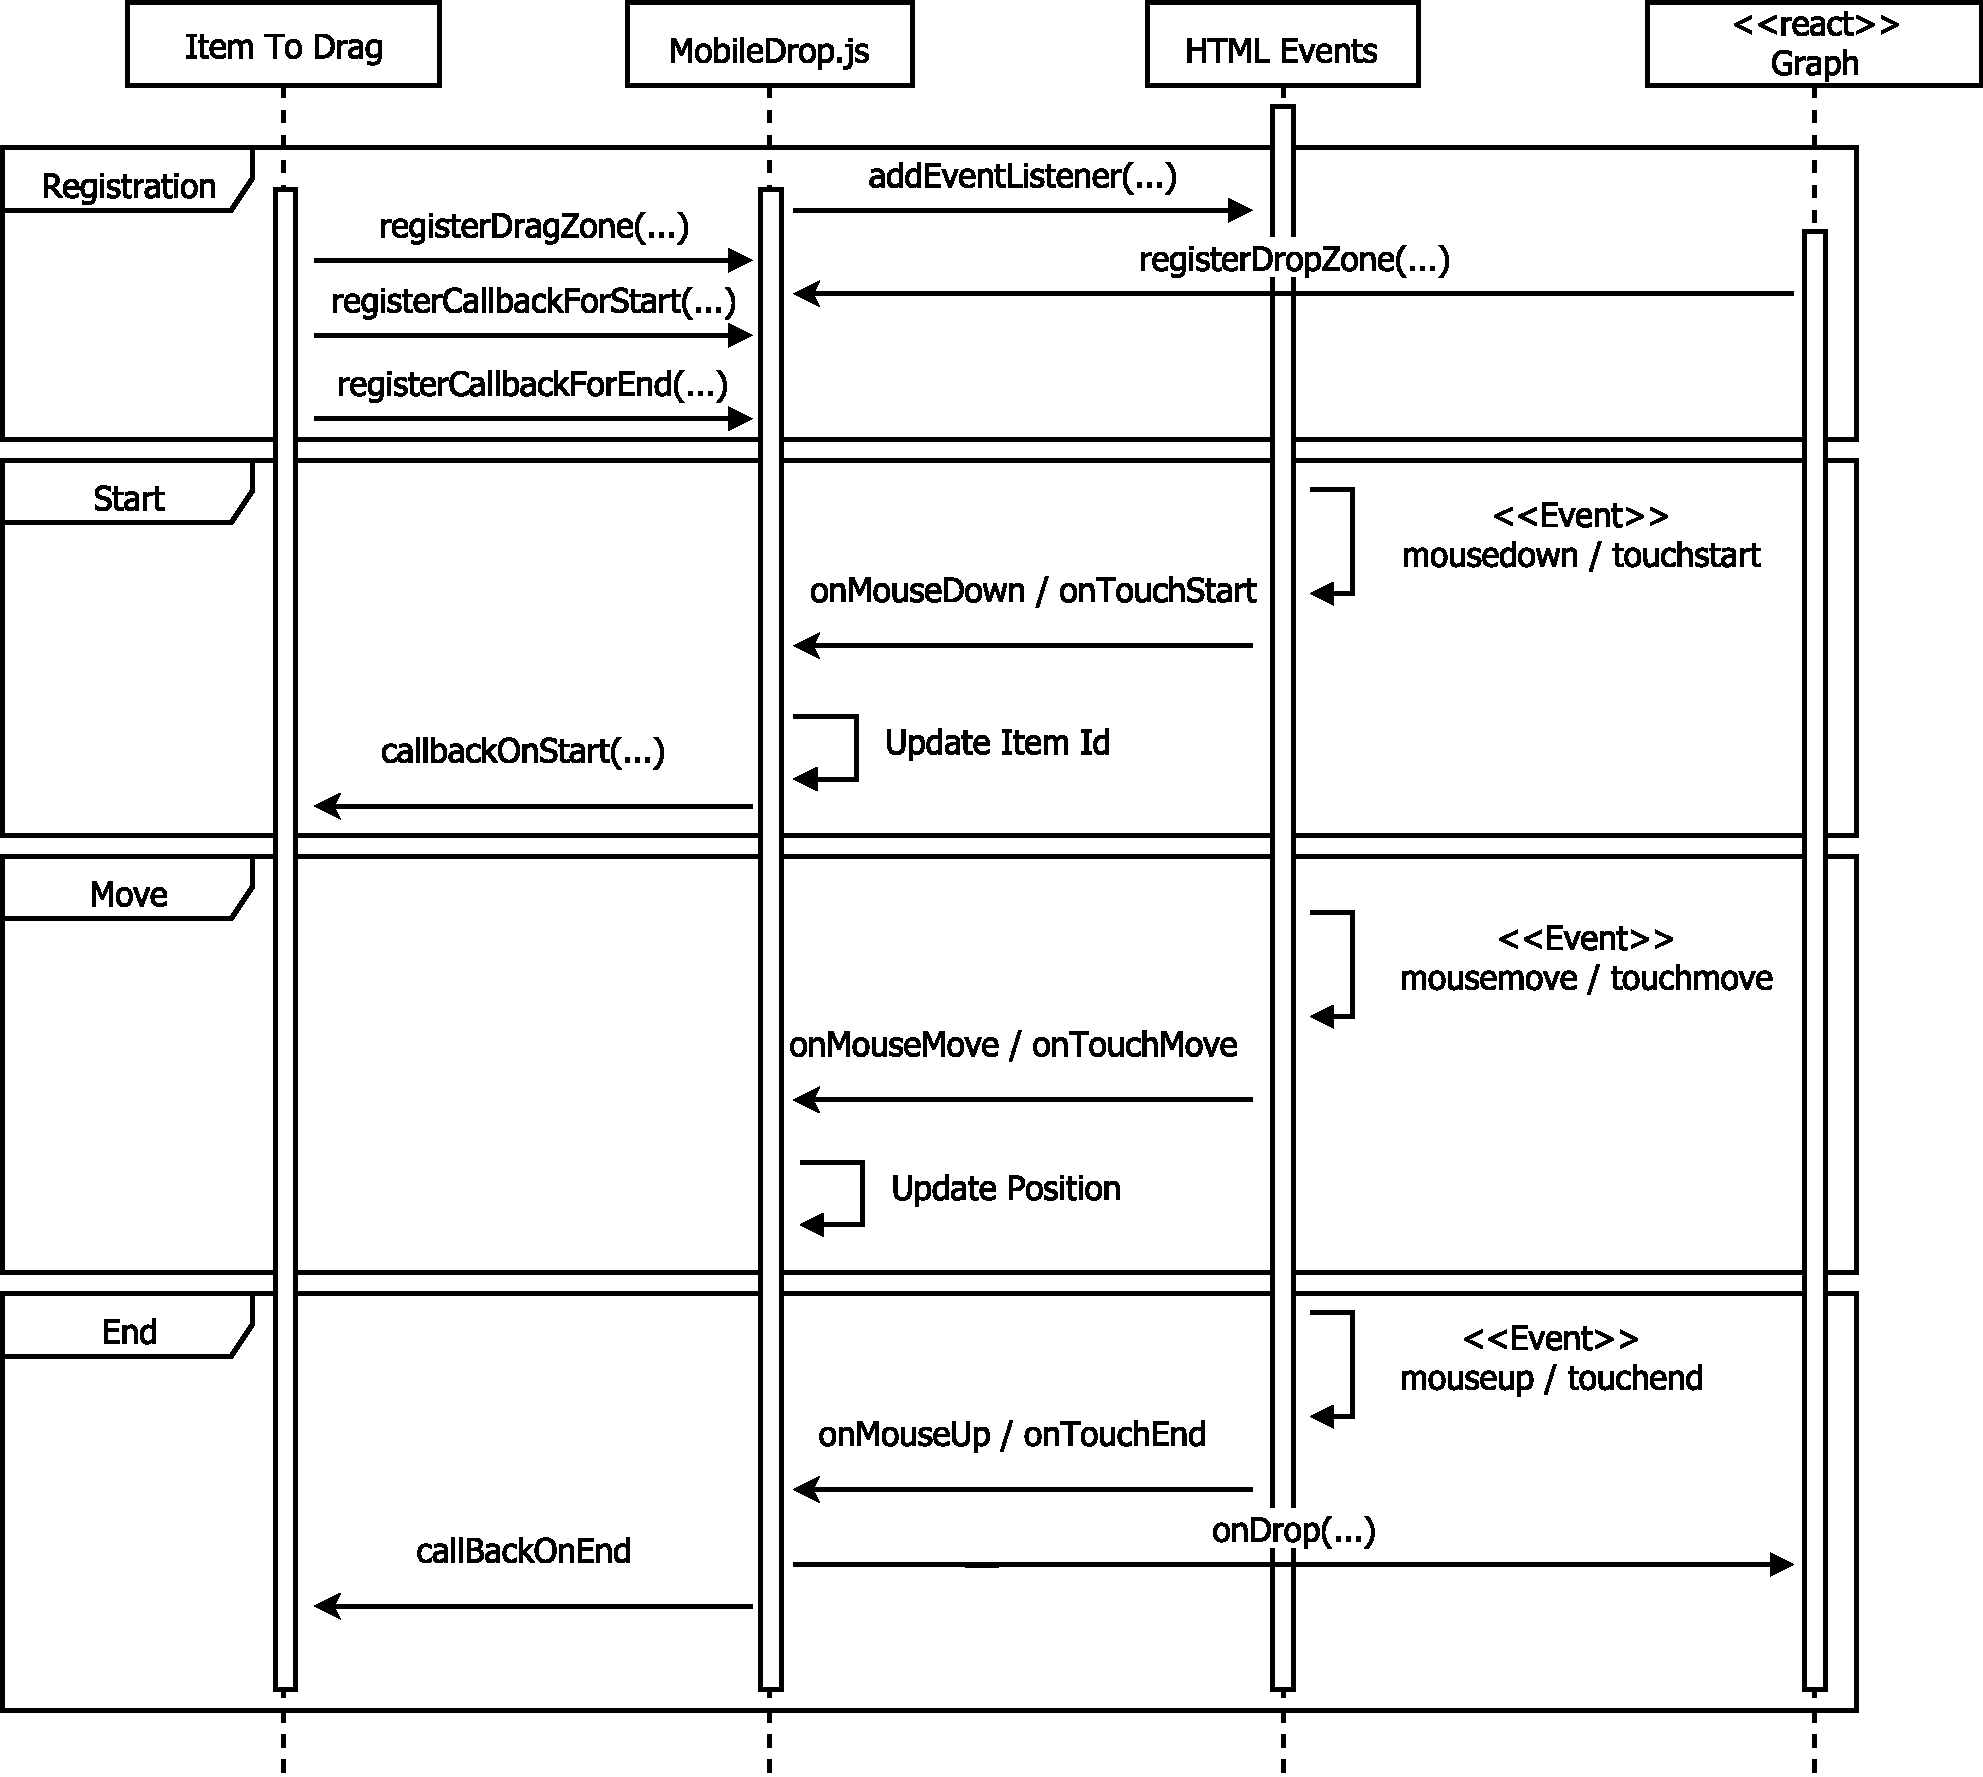
\includegraphics[width=1.2\textwidth]{DragAndDrop}}
\caption{Ablauf \gls{Drag'n'Drop}}
\label{fig:dnd-sequence}
\end{figure}

\section{Visualisierung}\label{visual}
Die Funktionalitäten der Visualisierung werden hauptsächlich durch vier \hyperref[react]{\textit{React}}-Komponenten abgedeckt: \textit{GraphScreen} fungiert dabei als zentrale Stelle und initialisiert alle anderen Komponenten. Insbesondere wird das entsprechende \hyperref[view]{\textit{View}}-Objekt, \textit{viewToLoad} analysiert, die darzustellenden \gls{Node}[s] und \gls{Link}[s] extrahiert und der \textit{Graph}-Komp\-on\-en\-te übergeben.

Sobald innerhalb der Visualisierung ein \gls{Event} aufgrund einer Benutzerinterkation ausgelöst wird, werden die entsprechenden \gls{Callback}-Methoden des \textit{GraphScreen} aufgerufen. Darüber werden die entsprechenden Schritte ausgeführt, welche wiederum zu Aktualisierungen in den einzelnen Komponenten führen (\autoref{fig:component-visualisation}). Jegliche Kommunikation zwischen den Komponenten wird nach dem Prinzip des unidirektionalen Datenflusses (\autoref{unidirectional}) realisiert.

Zum Beispiel soll ein \gls{Link} dargestellt werden. Dazu wird im \textit{GraphScreen} beim entsprechenden \hyperref[GraphLinkElement]{Link} die Eigenschaft \textit{visible} auf \texttt{VISI\-BILI\-TY.VISI\-BLE} gesetzt. Durch die Aktualisierung des Zustands werden nun die \gls{Node}[s] und \gls{Link}[s], welche der \textit{Graph}-Komponente übergeben werden, aktualisiert. Darin enthalten ist nun auch der neu darzustellende Link.

\begin{figure}[htbp]
\centerline{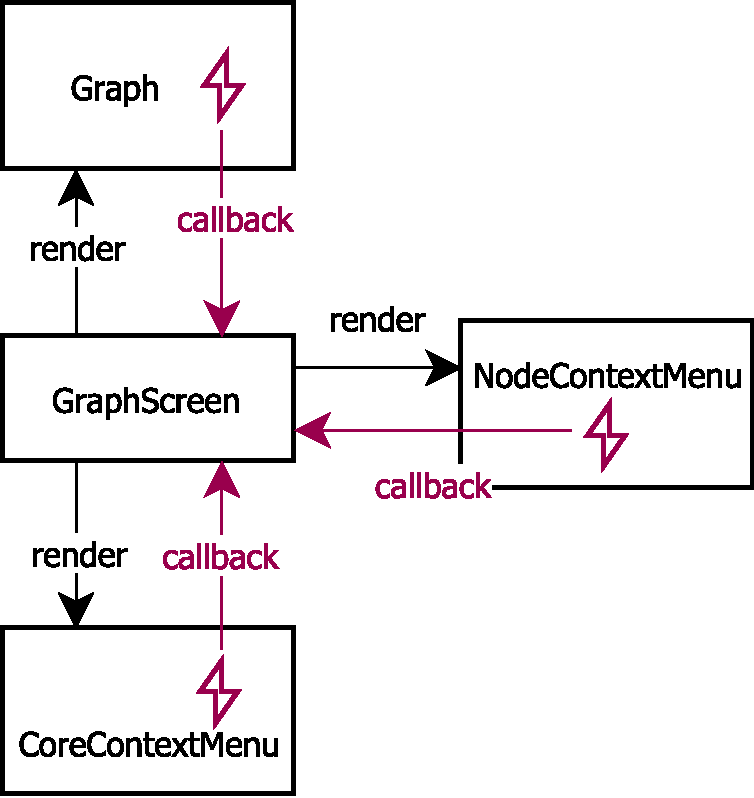
\includegraphics[width=0.5\textwidth]{VisualisationComponents}}
\caption{Komponenten der Visualisierung}
\label{fig:component-visualisation}
\end{figure}


\subsection{Manipulation des \gls{Netzwerk}[s]}
\label{subsec:graph-manipulation}

Die Manipulationen innerhalb des \gls{Netzwerk}[s] haben ihren Ursprung immer im \textit{cytoscape}-Framework. Hier werden verschiedene \gls{Event}s registriert, um entsprechend reagieren zu können. Dies geschieht auf verschiedenen Ebenen der Visualisierung:
\begin{enumerate}
    \item Auf der ganzen Visualisierung, zum Beispiel \textit{Rechtsklick} an einer freien Stelle.
    \item Auf mehreren \gls{Node}[s] der Visualisierung, zum Beispiel \textit{durch Auswahl}.
    \item Auf mehreren \gls{Link}[s] der Visualisierung, zum Beispiel durch \textit{Auswahl}.
    \item Auf einem spezifischen Element der Visualisierung, zum Beispiel \textit{Loslassen} eines \gls{Node}[s].
\end{enumerate}


\begin{listing}[htbp]
\inputminted[
frame=lines,
framesep=2mm,
baselinestretch=1.2,
linenos,
breaklines=true
]{js}{sourcecode/common/cytoscape-event.ts}
\caption{Cytoscape Event Beispiel}
\label{listing:cytoscape-event}
\end{listing}

\subsubsection{Update Position/New Link (Drag'n'Drop)}
Wenn die Aktion \textit{Update Position} und \textit{New Link} per \gls{Drag'n'Drop} ausgeführt werden, startet ein teilweise ähnlicher Ablauf (\autoref{fig:sequence-movenode}):
\begin{enumerate}
    \item Der erste Schritt ist Teil des allgemeinen Ablaufs der Visualisierung. Darin wird die \textit{Graph}-Komponente erstellt. Falls eine Aktion auf einem \gls{Node} ausgeführt wird, wird der \gls{Event} \textit{grab} registriert.
    \item Bei der Auswahl und Bewegung eines \gls{Node}[s], wird nun der \gls{Event} \textit{free} temporär registriert, welcher ausgeführt wird sobald der \gls{Node} losgelassen wird.
    \item Sobald der \gls{Node} losgelassen wird, wird überprüft, ob an dieser Stelle in der Visualisierung ein anderer \gls{Node} positioniert ist. Ist dies der Fall, wird ein neuer \gls{Link} zwischen den zwei \gls{Node}[s] erstellt und dazu folgende Schritte ausgeführt:  
        \begin{itemize}
            \item Die \textit{GraphScreen}-Komponente wird mittels einer \textit{Callback}-Meth\-ode informiert.
            \item Innerhalb der \textit{GraphScreen}-Komponente wird der neue \gls{Link} erstellt und die Datenbasis durch den \hyperref[OperationService]{\textit{OperationService}} informiert.
            \item Nun wird der Zustand der \textit{GraphScreen}-Komponente aktualisiert, die \texttt{render}-Methode ausgeführt und die Aktualisierungen an die \textit{Graph}-Komponente weitergegeben. Zum Schluss werden die Änderungen angezeigt.    
        \end{itemize}
    Wenn dies jedoch nicht zutrifft, werden folgende Schritte ausgeführt. So kann die neue Position des \gls{Node}[s] gespeichert werden: 
        \begin{itemize}
            \item Durch die entsprechende \textit{Callback}-Methode wird die \textit{GraphScreen}-Komponente informiert.
            \item Die Position wird innerhalb der \textit{GraphScreen}-Komponente aktualisiert und die Datenbasis durch den \hyperref[OperationService]{\textit{OperationService}} informiert.
            \item Ebenfalls wird der Zustand der \textit{GraphScreen}-Komponente aktualisiert, die \texttt{render} Methode ausgeführt und die Aktualisierungen an die \textit{Graph}-Komponente weitergegeben. Wiederum werden zum Schluss die Änderungen sichtbar.
        \end{itemize}
\end{enumerate}

\begin{figure}[htbp]
\centerline{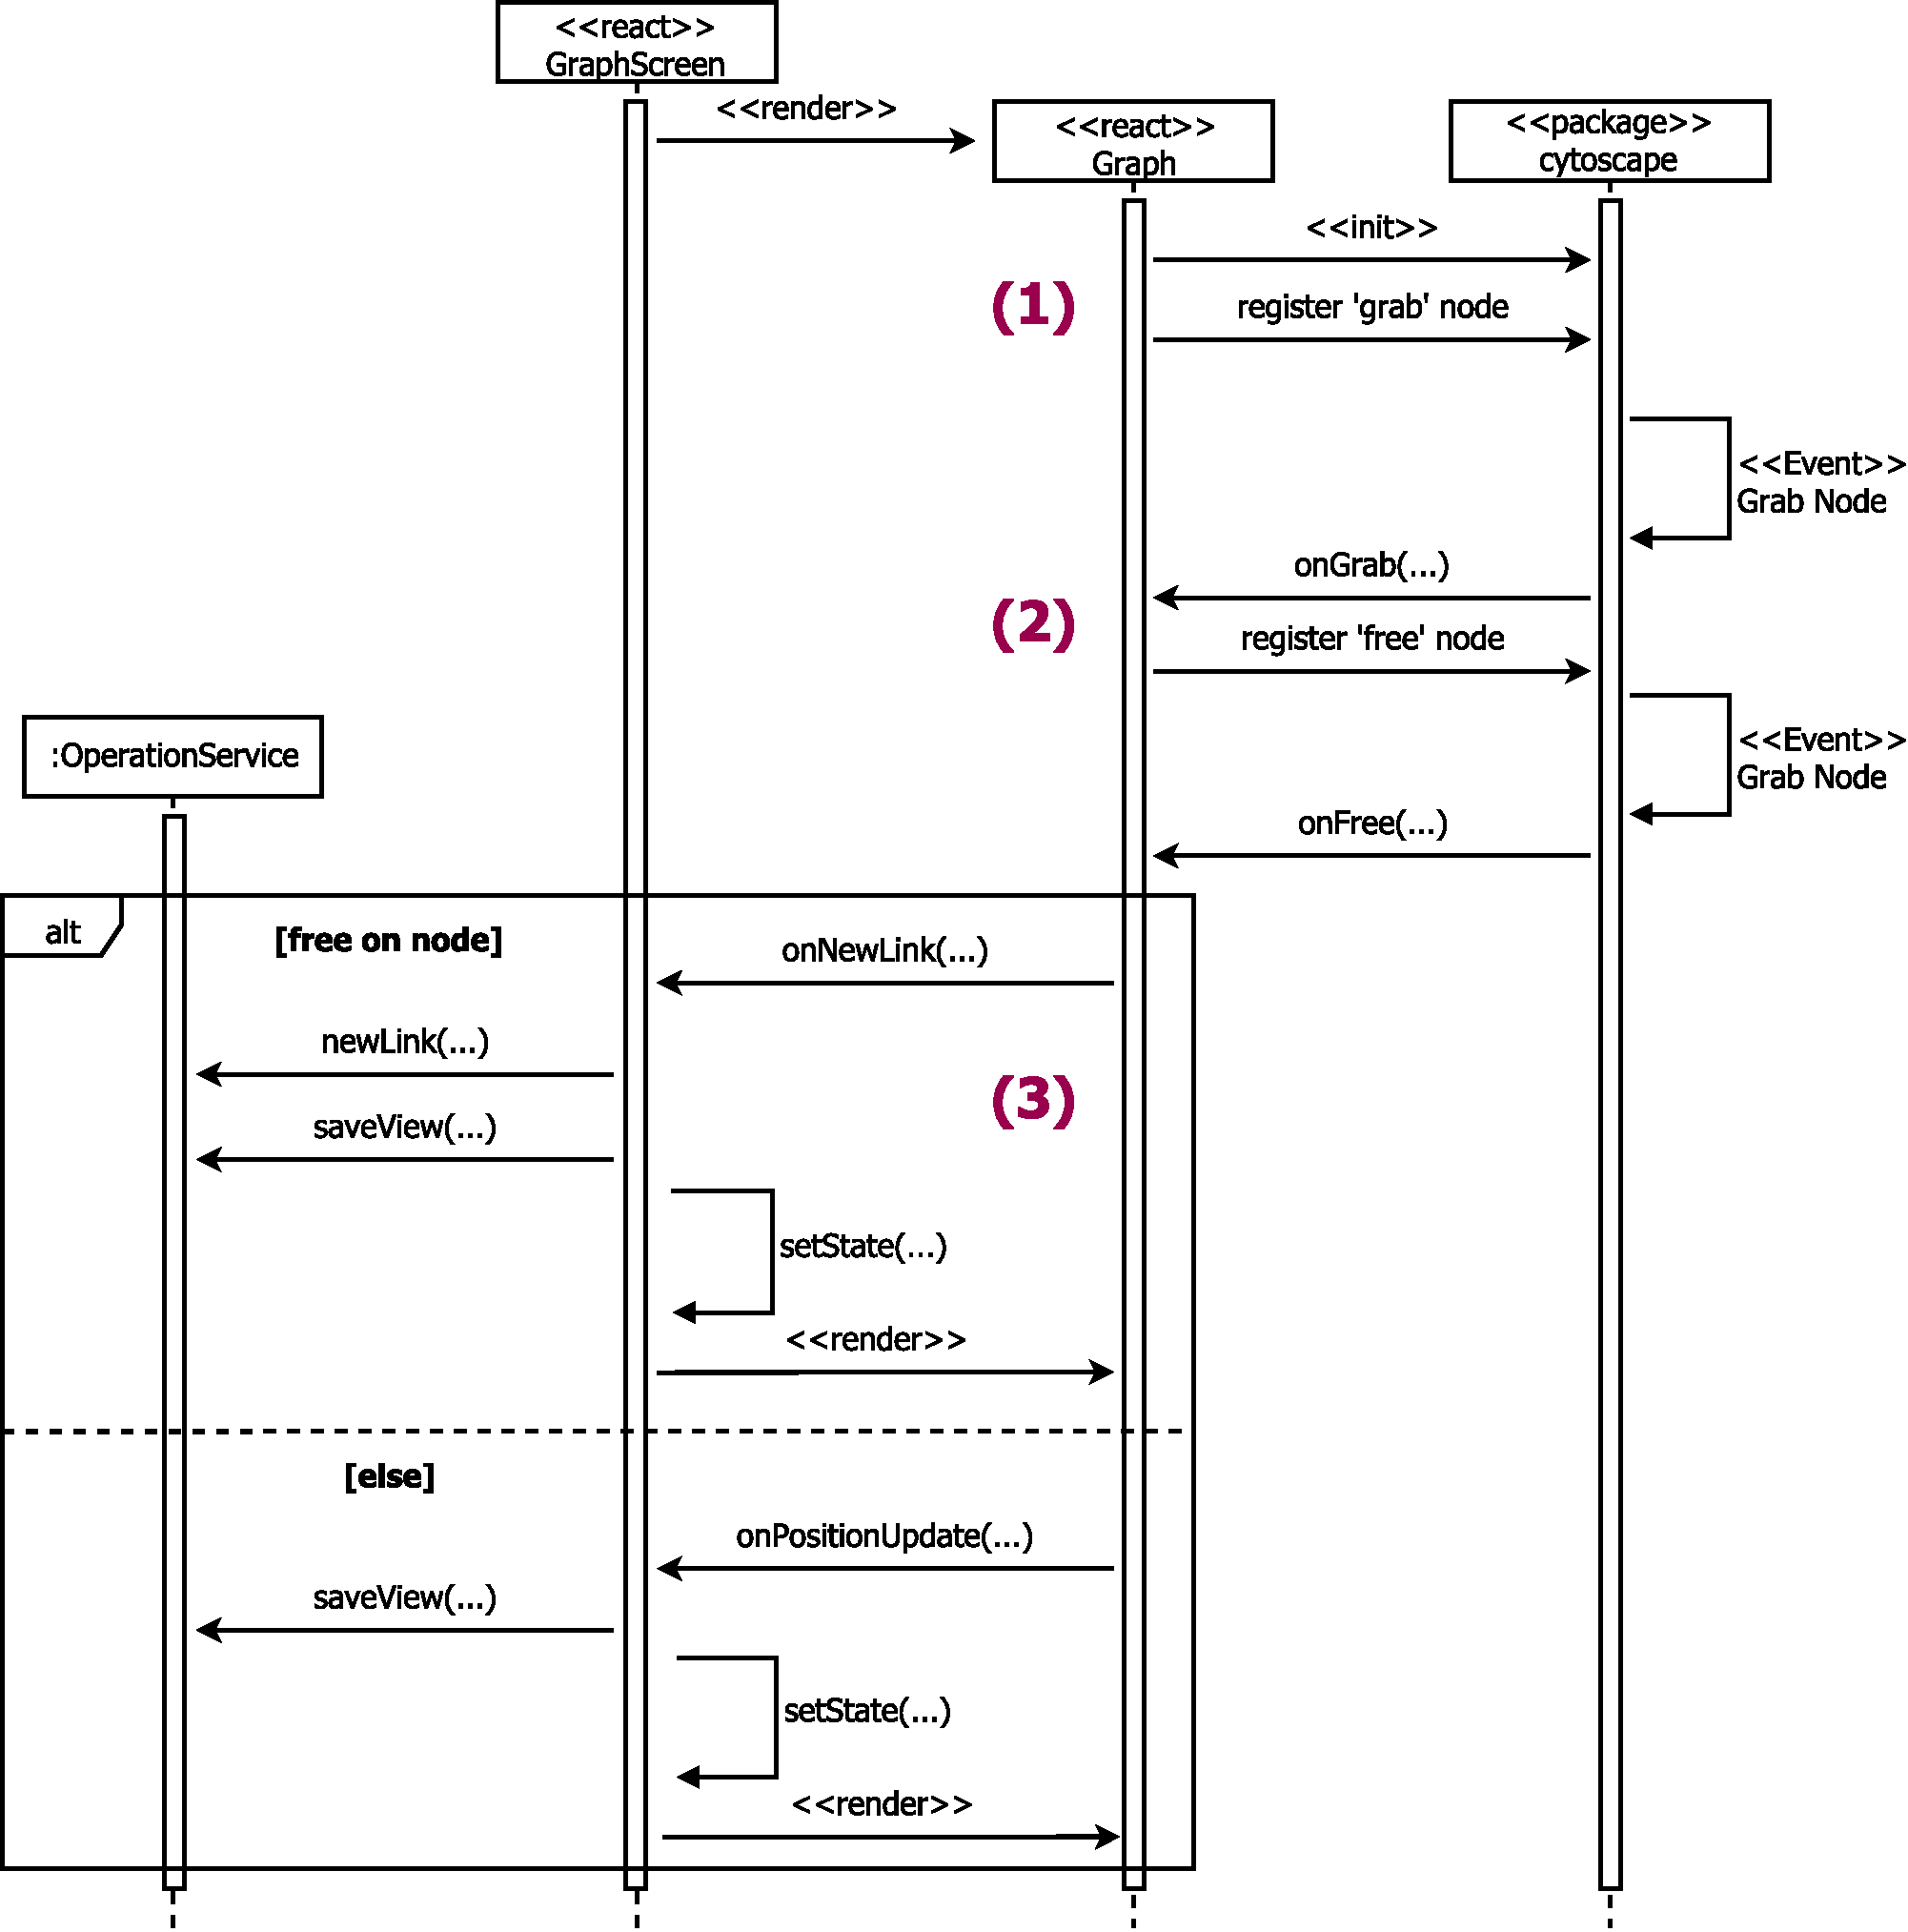
\includegraphics[width=1.2\textwidth]{UpdatePositionDiagramm}}
\caption{Ablauf Update Position / New Link}
\label{fig:sequence-movenode}
\end{figure}

\subsubsection{Add Node/Link To Existing \gls{Node} (Drag'n'Drop)}
Im \autoref{dnd} wurde bereits erläutert, wie ein \gls{Drag'n'Drop} eines \gls{Node}[s] von ausserhalb behandelt wird. Dadurch wird es ermöglicht, die Aktionen \textit{AddNode} und \textit{LinkToExistingNode} per \textit{Drag'n'Drop} auszuführen. Dazu werden weitere Schritte ausgeführt, welche auf diejenigen in der \autoref{fig:dnd-sequence} folgen (\autoref{fig:sequence-afterdrop}):
\begin{enumerate}
    \item Auch bei diesen beiden Aktionen werden zuerst die allgemeinen Schritte abgearbeitet und die Visualisierung als \textit{DropZone} registriert (vgl. \autoref{listing:dnd-handling}).  
    \item Sobald nun ein \gls{Node} über der Visualisierung losgelassen wird, wird die \textit{Graph}-Komponente informiert. 
    \item Anhand der Position des losgelassenen \gls{Node}[s] wird nun ermittelt, ob an dieser Stelle bereits ein \gls{Node} in der Visualisierung dargestellt wird. Falls dies zutrifft, muss der losgelassene \gls{Node} in der Visualisierung dargestellt werden und mit einem \gls{Link} zum \gls{Node} an der losgelassenen Stelle verbunden werden. Dafür sind folgenden Schritte notwendig:
        \begin{itemize}
            \item Mithilfe der entsprechenden \textit{Callback}-Methode wird die \textit{GraphScreen}-Komponente informiert.
            \item Die Änderungen werden nun in der \textit{GraphScreen}-om\-po\-nen\-te ausgeführt und die Datenbasis durch den \hyperref[OperationService]{\textit{OperationService}} informiert.
            \item Durch die Aktualisierung des Zustands der \textit{GraphScreen}-Komponente wird die \texttt{render}-Methode ausgeführt und die Aktualisierungen an die \textit{Graph}-Komponente weitergegeben und somit die Änderungen angezeigt.    
        \end{itemize}
    Wenn nun der \gls{Node} an einer freien Stelle losgelassen wird, soll dieser ohne einen neuen \gls{Link} erstellt werden. Dazu sind folgende Schritte nötig:
        \begin{itemize}
            \item Durch die entsprechenden \textit{Callback}-Methode wird die Information an die \textit{GraphScreen}-Komponente weitergegeben.
            \item Änderungen werden nun innerhalb der \textit{GraphScreen}-Kom\-po\-nen\-te abgearbeitet und die Informationen durch den \hyperref[OperationService]{\textit{OperationService}} an die Datenbasis weitergegeben.
            \item Auch hier wird zum Schluss die Aktualisierung des Zustands der \textit{GraphScreen}-Komponente ausgeführt und somit die \texttt{render}-Methode aufgerufen. Die Aktualisierungen werden an die \textit{Graph}-Komponente weitergegeben und somit die Änderungen angezeigt.    
        \end{itemize}
\end{enumerate}
\begin{figure}[htbp]
\centerline{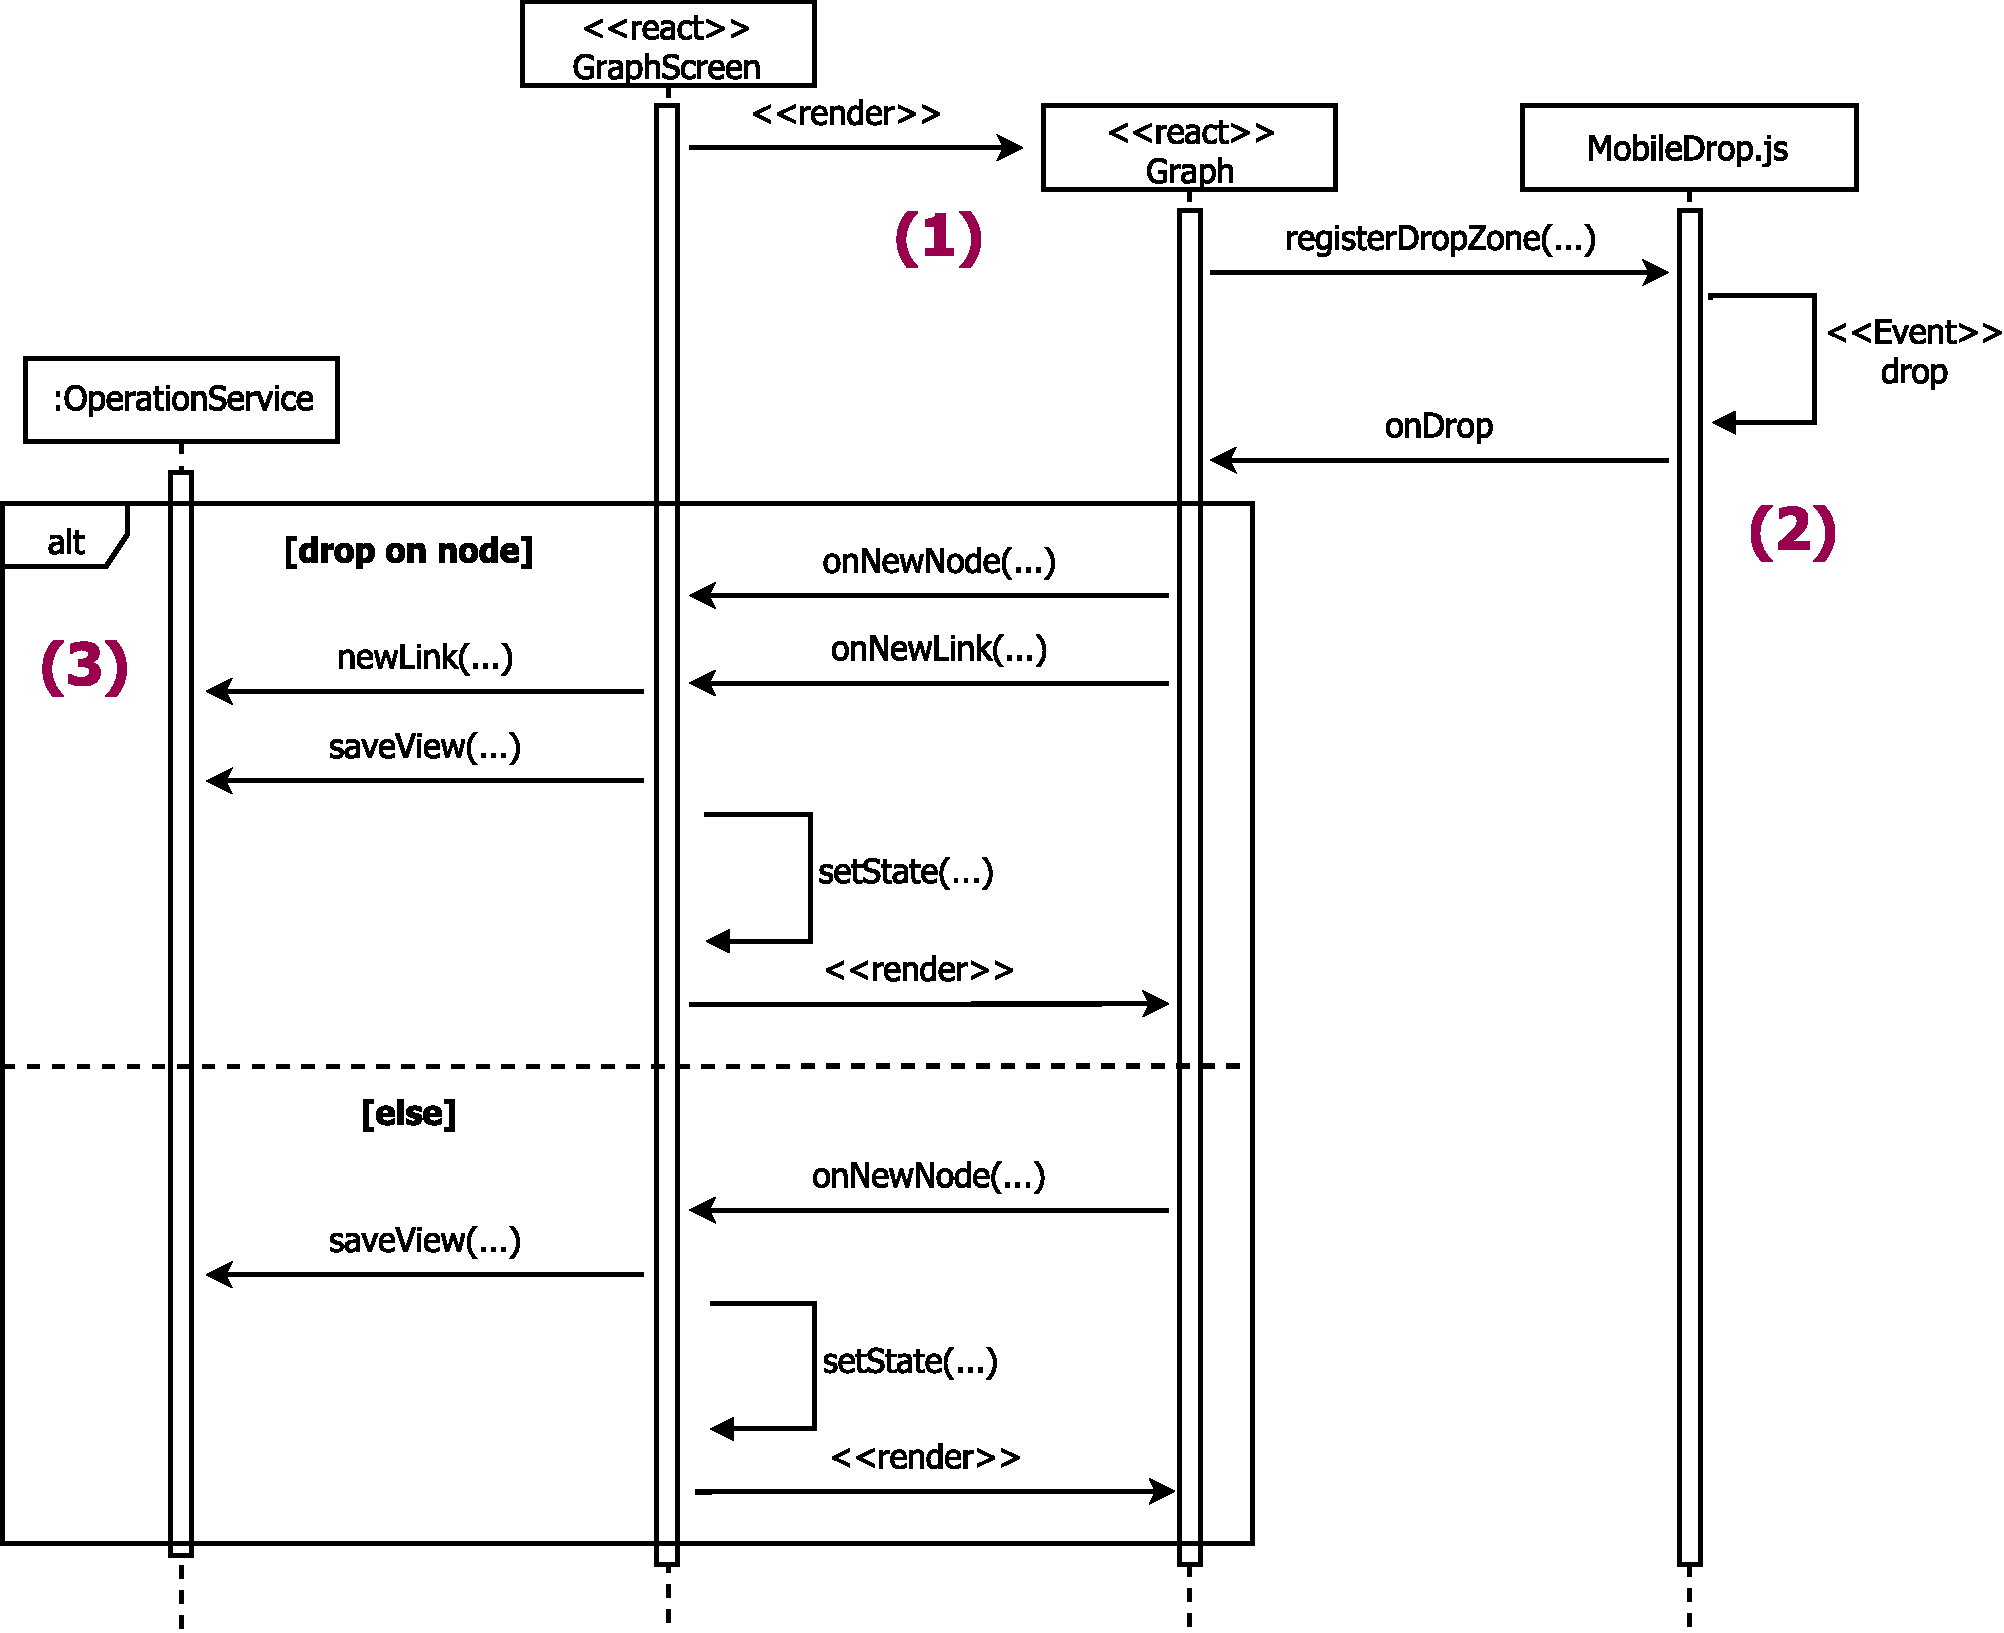
\includegraphics[width=1.2\textwidth]{FurtherProcessDropNode}}
\caption{Ablauf Add Node / Link To Existing Node}
\label{fig:sequence-afterdrop}
\end{figure}


\subsection{Kontextmenüs}
Die beiden Kontextmenüs (\autoref{fig:core-contextmenu} und \autoref{fig:node-contextmenu}) bieten eine Sammlung von \hyperref[subsec:aktionen]{\textit{Aktionen}}, welche der entsprechenden Situation angepasst sind. Beide werden entweder durch einen Rechtsklick (Desktop) oder einen langen Tap (Mobile) aufgerufen. Diese \gls{Event}s werden ebenfalls, wie in \autoref{visual} beschrieben, innerhalb der \textit{Graph}-Komponente beim \textit{cytoscape}-Framework registriert. Sobald der \gls{Event} auftritt werden durch die entsprechenden \textit{Callback}-Methoden die \textit{GraphScreen}-Komponente informiert, damit diese das entsprechende Menü öffnet.

Um die entsprechenden Suchfelder oder Dialoge aufzurufen, nutzen beide Menüs die Implementierung der Schnittstellen \hyperref[SearchFieldFactory]{SearchFieldFactory} oder \hyperref[DialogFactory]{DialogFactory} (\autoref{interaktion}).

\begin{figure}
\centering
\begin{subfigure}[b]{0.5\textwidth}
    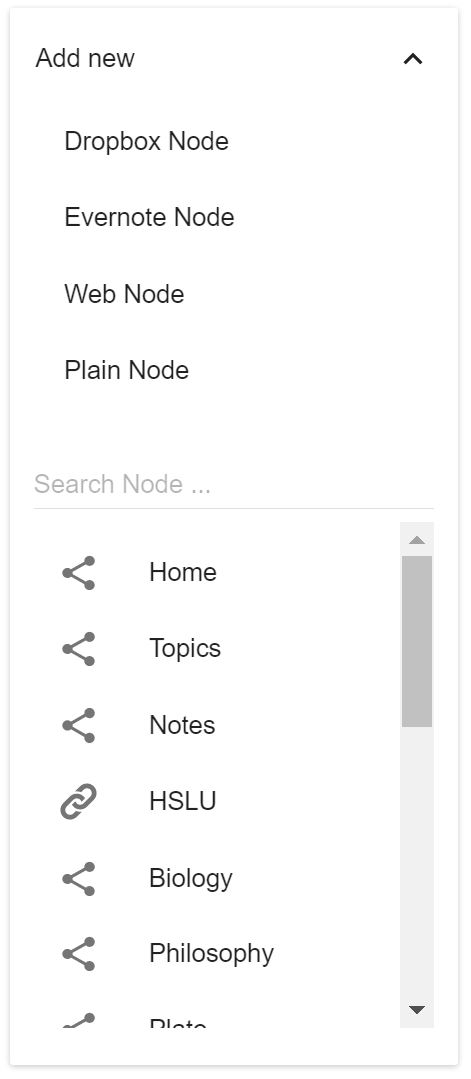
\includegraphics[width=1\linewidth]{CoreContextMenu-Screen}
    \caption{CoreContextMenu}
    \label{fig:core-contextmenu}
    \end{subfigure}
\begin{subfigure}[b]{0.4\textwidth}
    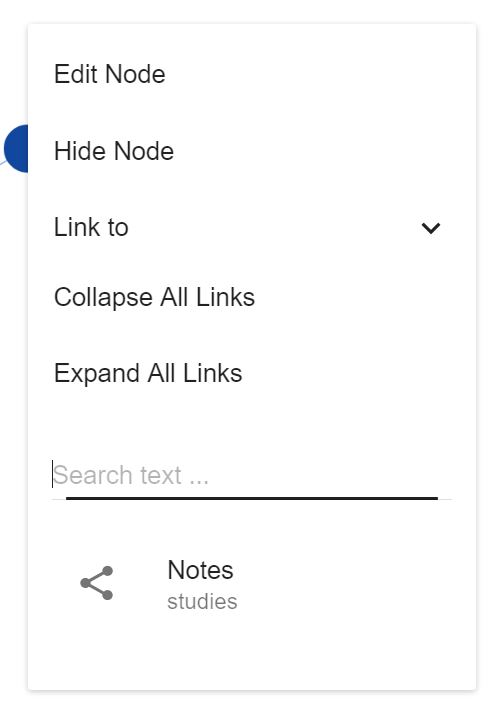
\includegraphics[width=1\linewidth]{NodeContextMenu-Screen}
    \caption{NodeContextMenu}
    \label{fig:node-contextmenu}
    \end{subfigure}
    \caption{Kontextmenüs}
\end{figure}


\subsubsection{CoreContextMenu}
Im \textit{CoreContextMenu} (\autoref{fig:core-contextmenu}) werden die beiden Aktionen \textit{AddNode} und \textit{NewNode} zur Verfügung gestellt (\autoref{subsec:aktionen}). Dabei werden durch die Implementierungen der beiden Schnittstellen \hyperref[SearchFieldFactory]{SearchFieldFactory} und \hyperref[DialogFactory]{DialogFactory} das Suchfeld \textit{GraphNodeSearchField} und der Dialog \textit{NewNodeDialog} bezogen und eingebunden (\autoref{fig:sequence-corecontextmenu}).

\begin{figure}[htbp]
\centerline{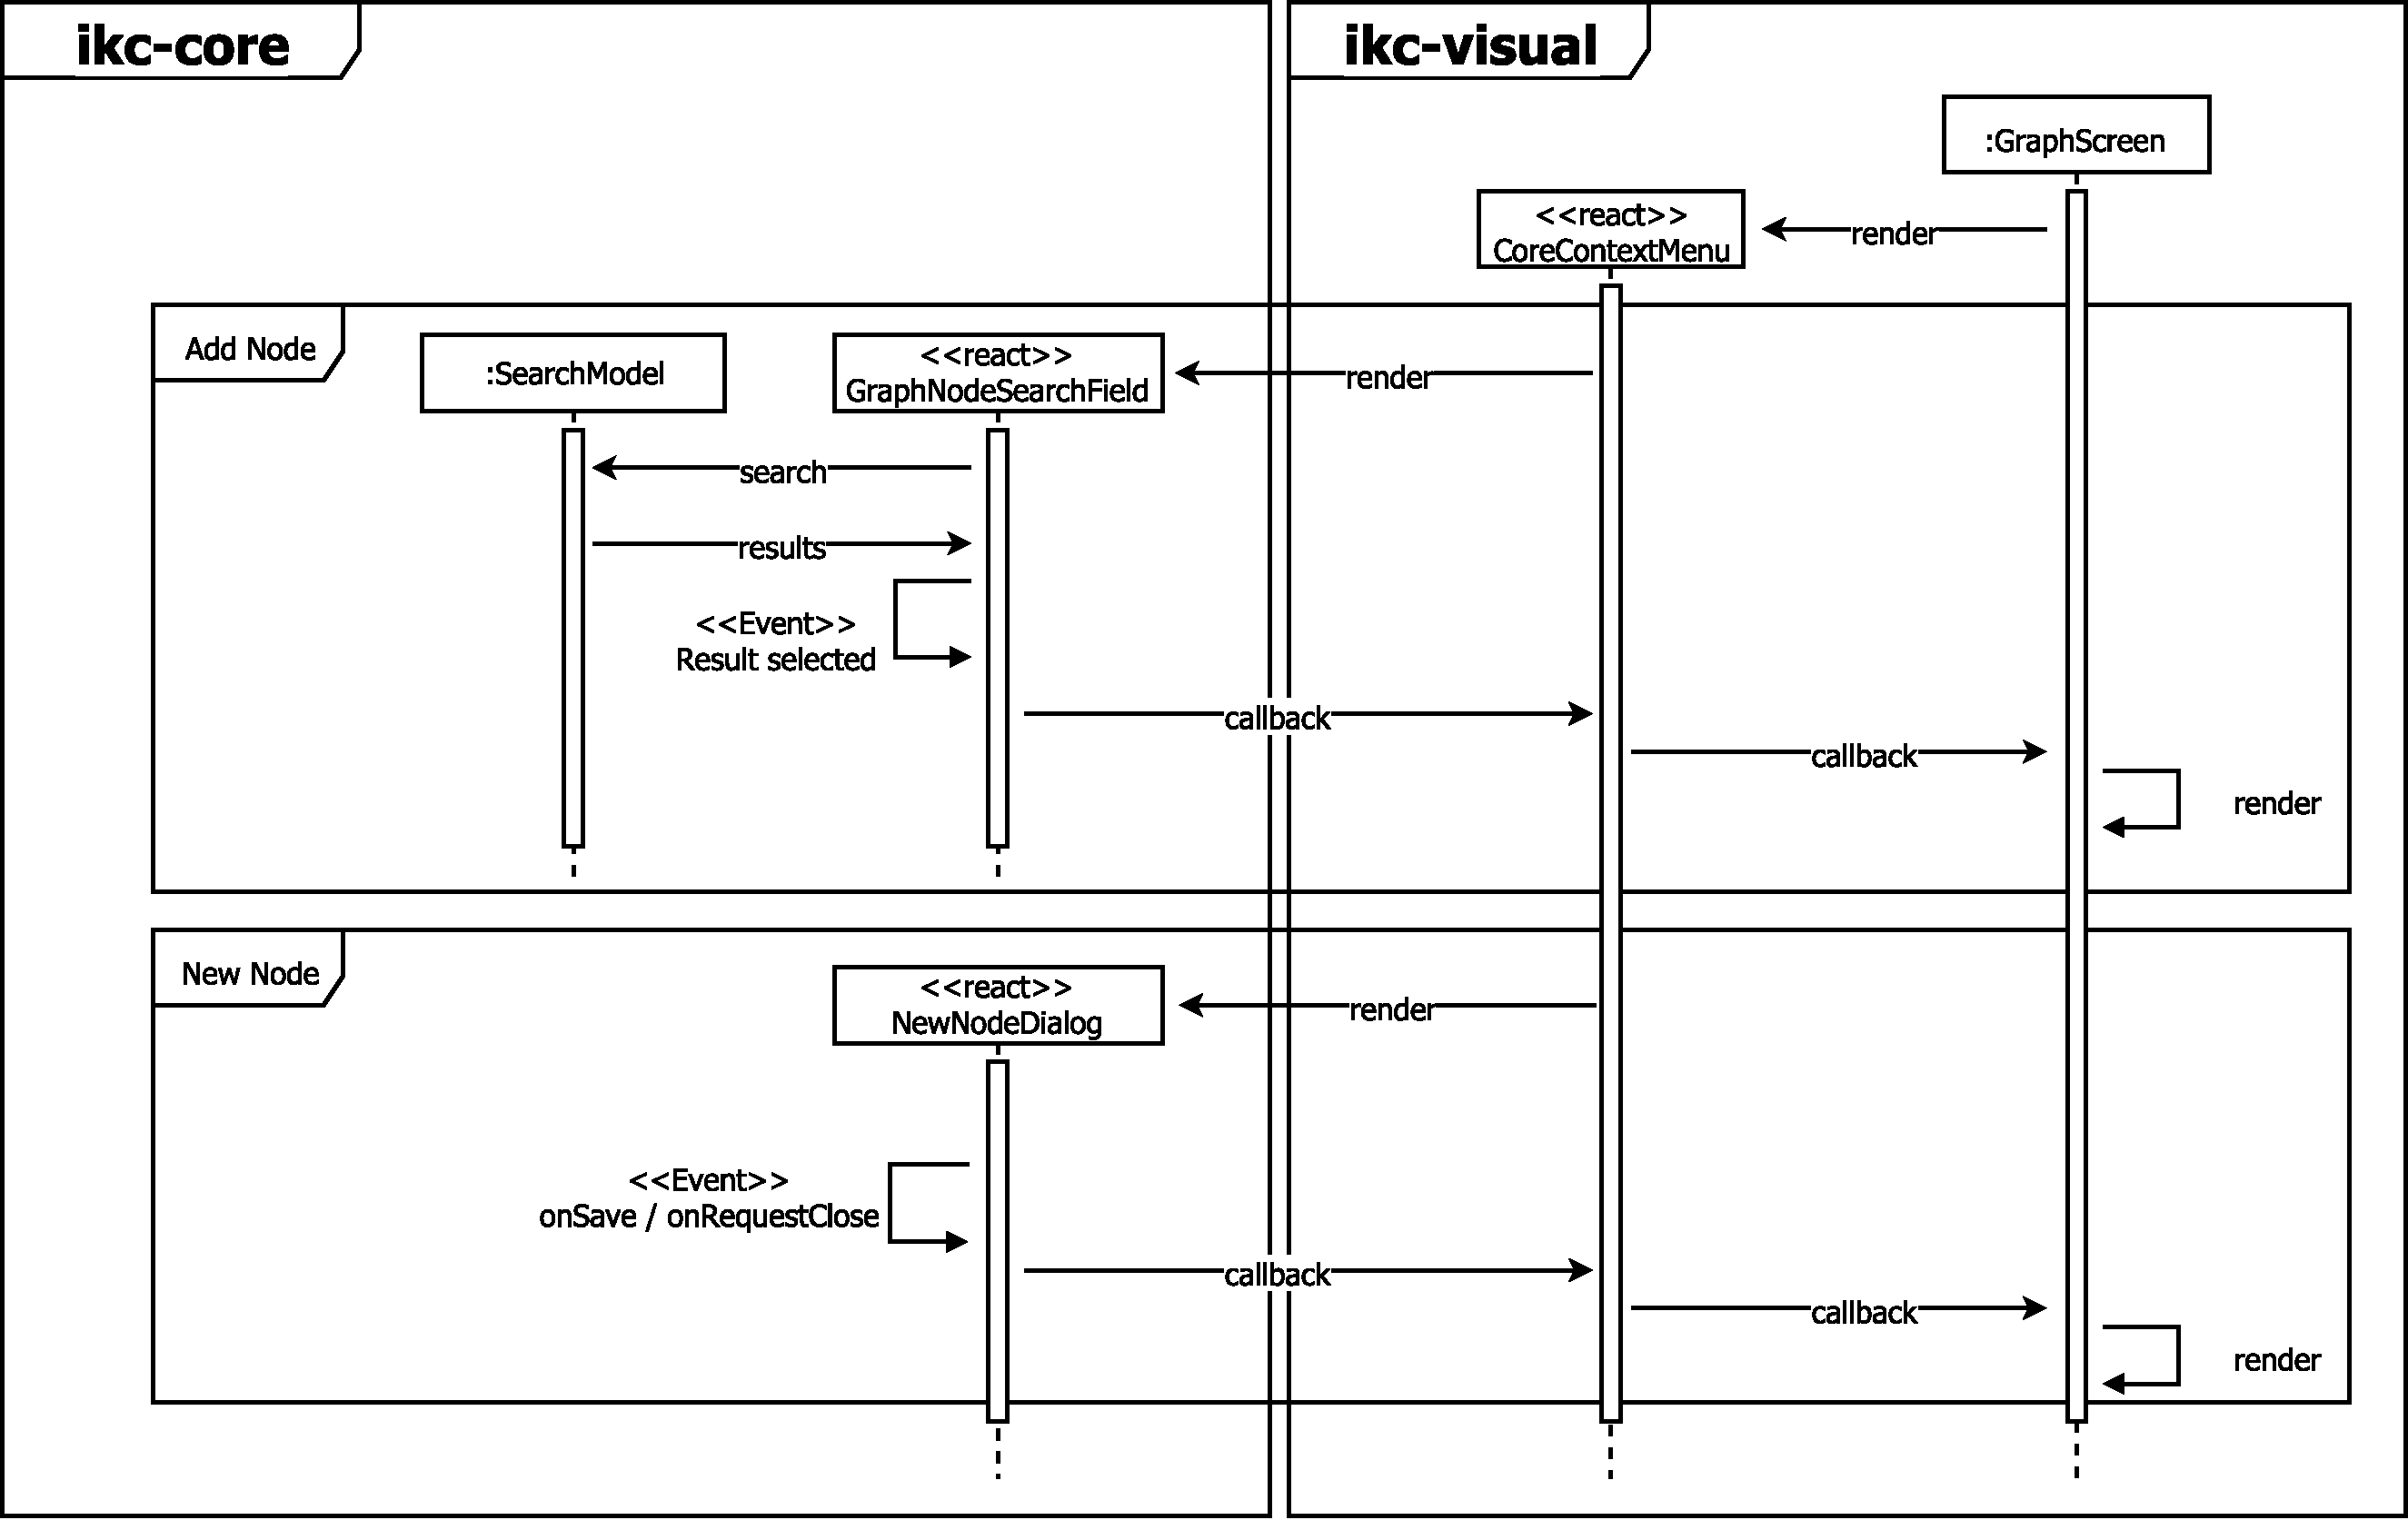
\includegraphics[width=1.2\textwidth]{CoreContextMenuSequence}}
\caption{Ablauf CoreContextMenu}
\label{fig:sequence-corecontextmenu}
\end{figure}


\subsubsection{NodeContextMenu}
Diverse \gls{Node} spezifische Aktionen werden im \textit{CoreContextMenu} zusammengefasst (\autoref{subsec:aktionen}). Dazu werden ebenfalls mithilfe der Implementierungen der beiden Schnittstellen \hyperref[SearchFieldFactory]{SearchFieldFactory} und \hyperref[DialogFactory]{DialogFactory} das Suchfeld \textit{GraphLinkSearchField} und die beiden Dialoge \textit{NewNodeToConnect} und \textit{ExistingNodeToConnect} genutzt (\autoref{fig:sequence-nodecontextmenu}). 
\begin{figure}[htbp]
\centerline{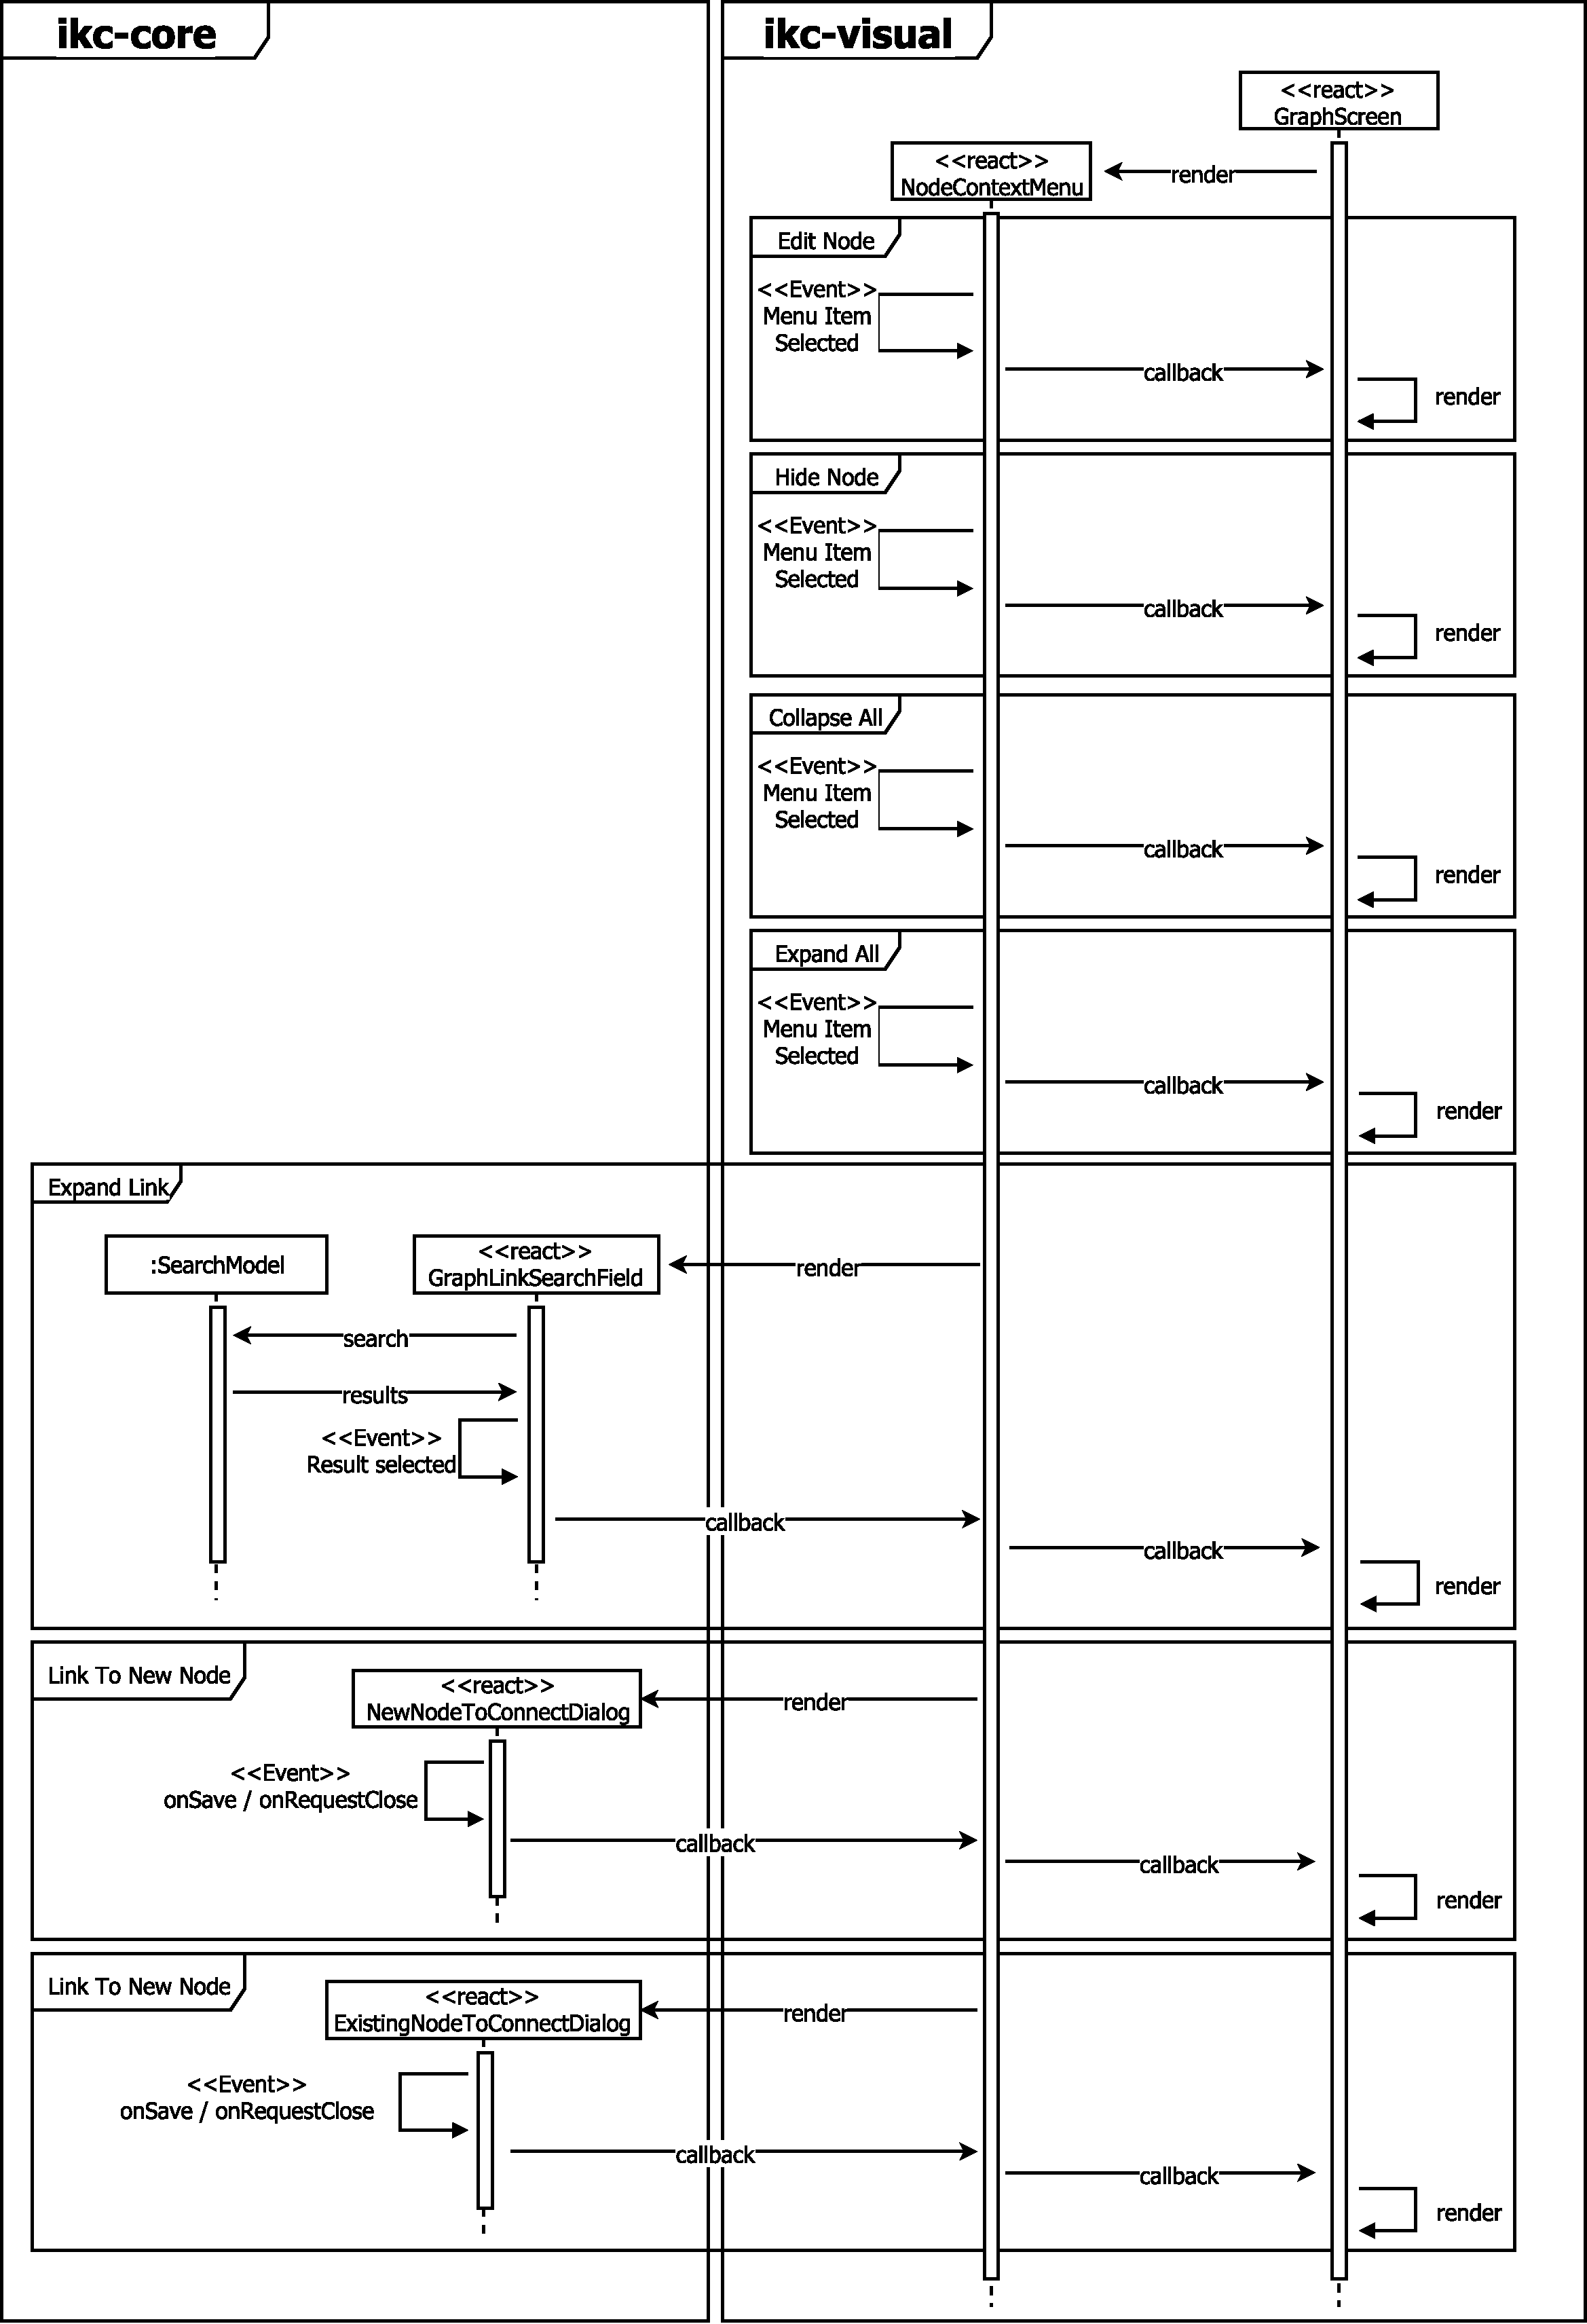
\includegraphics[width=1.15\textwidth]{NodeContextMenuSequence}}
\caption{Ablauf NodeContextMenu}
\label{fig:sequence-nodecontextmenu}
\end{figure}

\section{Integration}
Mit der Integration der Visualisierung in den \textit{ikc-core} wird die Implementation abgeschlossen. Dazu sind die nötigen Schnittstellen zu implementieren und zusätzlich weitere Anpassungen  (\autoref{fig:integration-visualisation}) notwendig:

\begin{itemize}
    \item \textit{GraphVisualisation} - nutzt die \textit{GraphScreen}-Komponente und üb\-er\-gi\-bt ihr alle nötigen Implementationen und Informationen. 
    \item \textit{GraphNodeInformationProvider} - ermöglicht der Visualisierung den Zugriff auf die Datenbasis, um Informationen abzufragen und implementiert die Schnittstelle \hyperref[NodeInformationProvider]{NodeInformationProvider}.
    \item \textit{GraphOperationService} - Dadurch kann die Visualisierung Informationen an die Datenbasis (\textit{NodeService}, \textit{PropertyService} und \textit{ViewService}) weiterleiten. Dazu wird die Schnittstelle \hyperref[OperationService]{OperationService} verwendet.
    \item \textit{GraphDialogFactory} - kapselt die Erstellung der verschiedene Dialog und stellt diese zur Verfügung. Es werden die verschiedenen Methoden der Schnittstelle \hyperref[DialogFactory]{DialogFactory} implementiert.
    \item \textit{GraphSearchFieldFactory} - um die beiden Suchfelder \textit{GraphNodeSearchField} und \textit{GraphLinkSearchField} der Visualisierung zu Ver\-füg\-ung zu stellen, wird die Schnittstelle \hyperref[SearchFieldFactory]{SearchFieldFactory} implementiert.
    \item \textit{ElementIdentityService} - damit die Visualisierung konsistente IDs für neue \gls{Node}[s] und \gls{Link}[s] vergeben kann, werden diese mithilfe der Schnittstelle \hyperref[IdentityService]{IdentityService} implementiert.
    \item \textit{Dialoge} - die verschiedenen Dialoge, welche der Visualisierung durch die \textit{GraphDialogFactory} zu Verfügung gestellt werden, nutzen die \hyperref[subsec:dialoginterfaces]{Dialog-Schnittstellen}. Diese dienen als Grundlage für die \gls{Props}- und \gls{State}-Schnittstellen der \hyperref[react]{\textit{React}}-Komponente.
    \item Um die verschiedenen \gls{View}s strukturiert halten zu können, werden die Klassen \textit{ViewService} und \textit{ViewModel} verwendet. Innerhalb des \textit{ViewModel}s wird auch die Verbindung zur externen Persistierung auf \gls{Dropbox} implementiert.
    \item Bisher wurde die Applikation nach folgendem Schema aufgerufen: \url{https://<host>/node/:node}, wobei \textit{:node} die darzustellende Node-ID enthält, z.B. \url{https://localhost:8888/node/0}. Neu wird das folgende Schema verwendet: \url{https://<host>/:node(/:view)(/:focus)}. Dabei wurden die beiden optionalen Parameter \textit{:view} und \textit{:focus} hinzugefügt. \textit{:view} enthält die entsprechende ID der View, welche darzustellen ist und \textit{:focus} den Wert \textit{node} oder \textit{view} je nachdem, auf welcher Darstellung der Fokus liegt. Dies ist jedoch nur auf der Mobile-Ansicht relevant. Mit dem Aufruf \url{https://localhost:8888/0/0/view} wird der \gls{Node} mit der ID \textit{0} und die Sicht mit der ID \textit{0} geladen, weiter soll der Fokus auf der Visualisierung liegen, falls die Anfrage von einem mobilen Gerät kommt.
    \item Der mobilen Navigationsleiste wurde ein neues Icon hinzugefügt, mit welchem zwischen der Visualisierung und der NodeDetail-Ansicht gewechselt werden kann. 
    \item Für die Navigation in der Mobile- und der Desktop-Ansicht wurde ein neuer Punkt \textit{View} hinzugefügt. Dadurch können neue Views erstellt, bestehende durchsucht und dargestellt werden. Weiter wurde dem Punkt \textit{Delete} zwei Menüpunkte \textit{DeleteView} und \textit{DeleteNode} hinzugefügt. 
    \item Innerhalb des \textit{NodeService} wurden entsprechende Methoden des \textit{ViewService} eingebaut. Somit wird sichergestellt, dass alle Änd\-er\-ung\-en der Datenbasis auch den verschiedenen Sichten weitergegeben werden. So zum Beispiel falls ein \gls{Link} in der Datenbasis gelöscht wird. Diese Änderung muss auch in den Views ausgeführt werden, sodass dieser \gls{Link} nicht mehr dargestellt wird. 
    
\end{itemize}

\begin{figure}[htbp]
\centerline{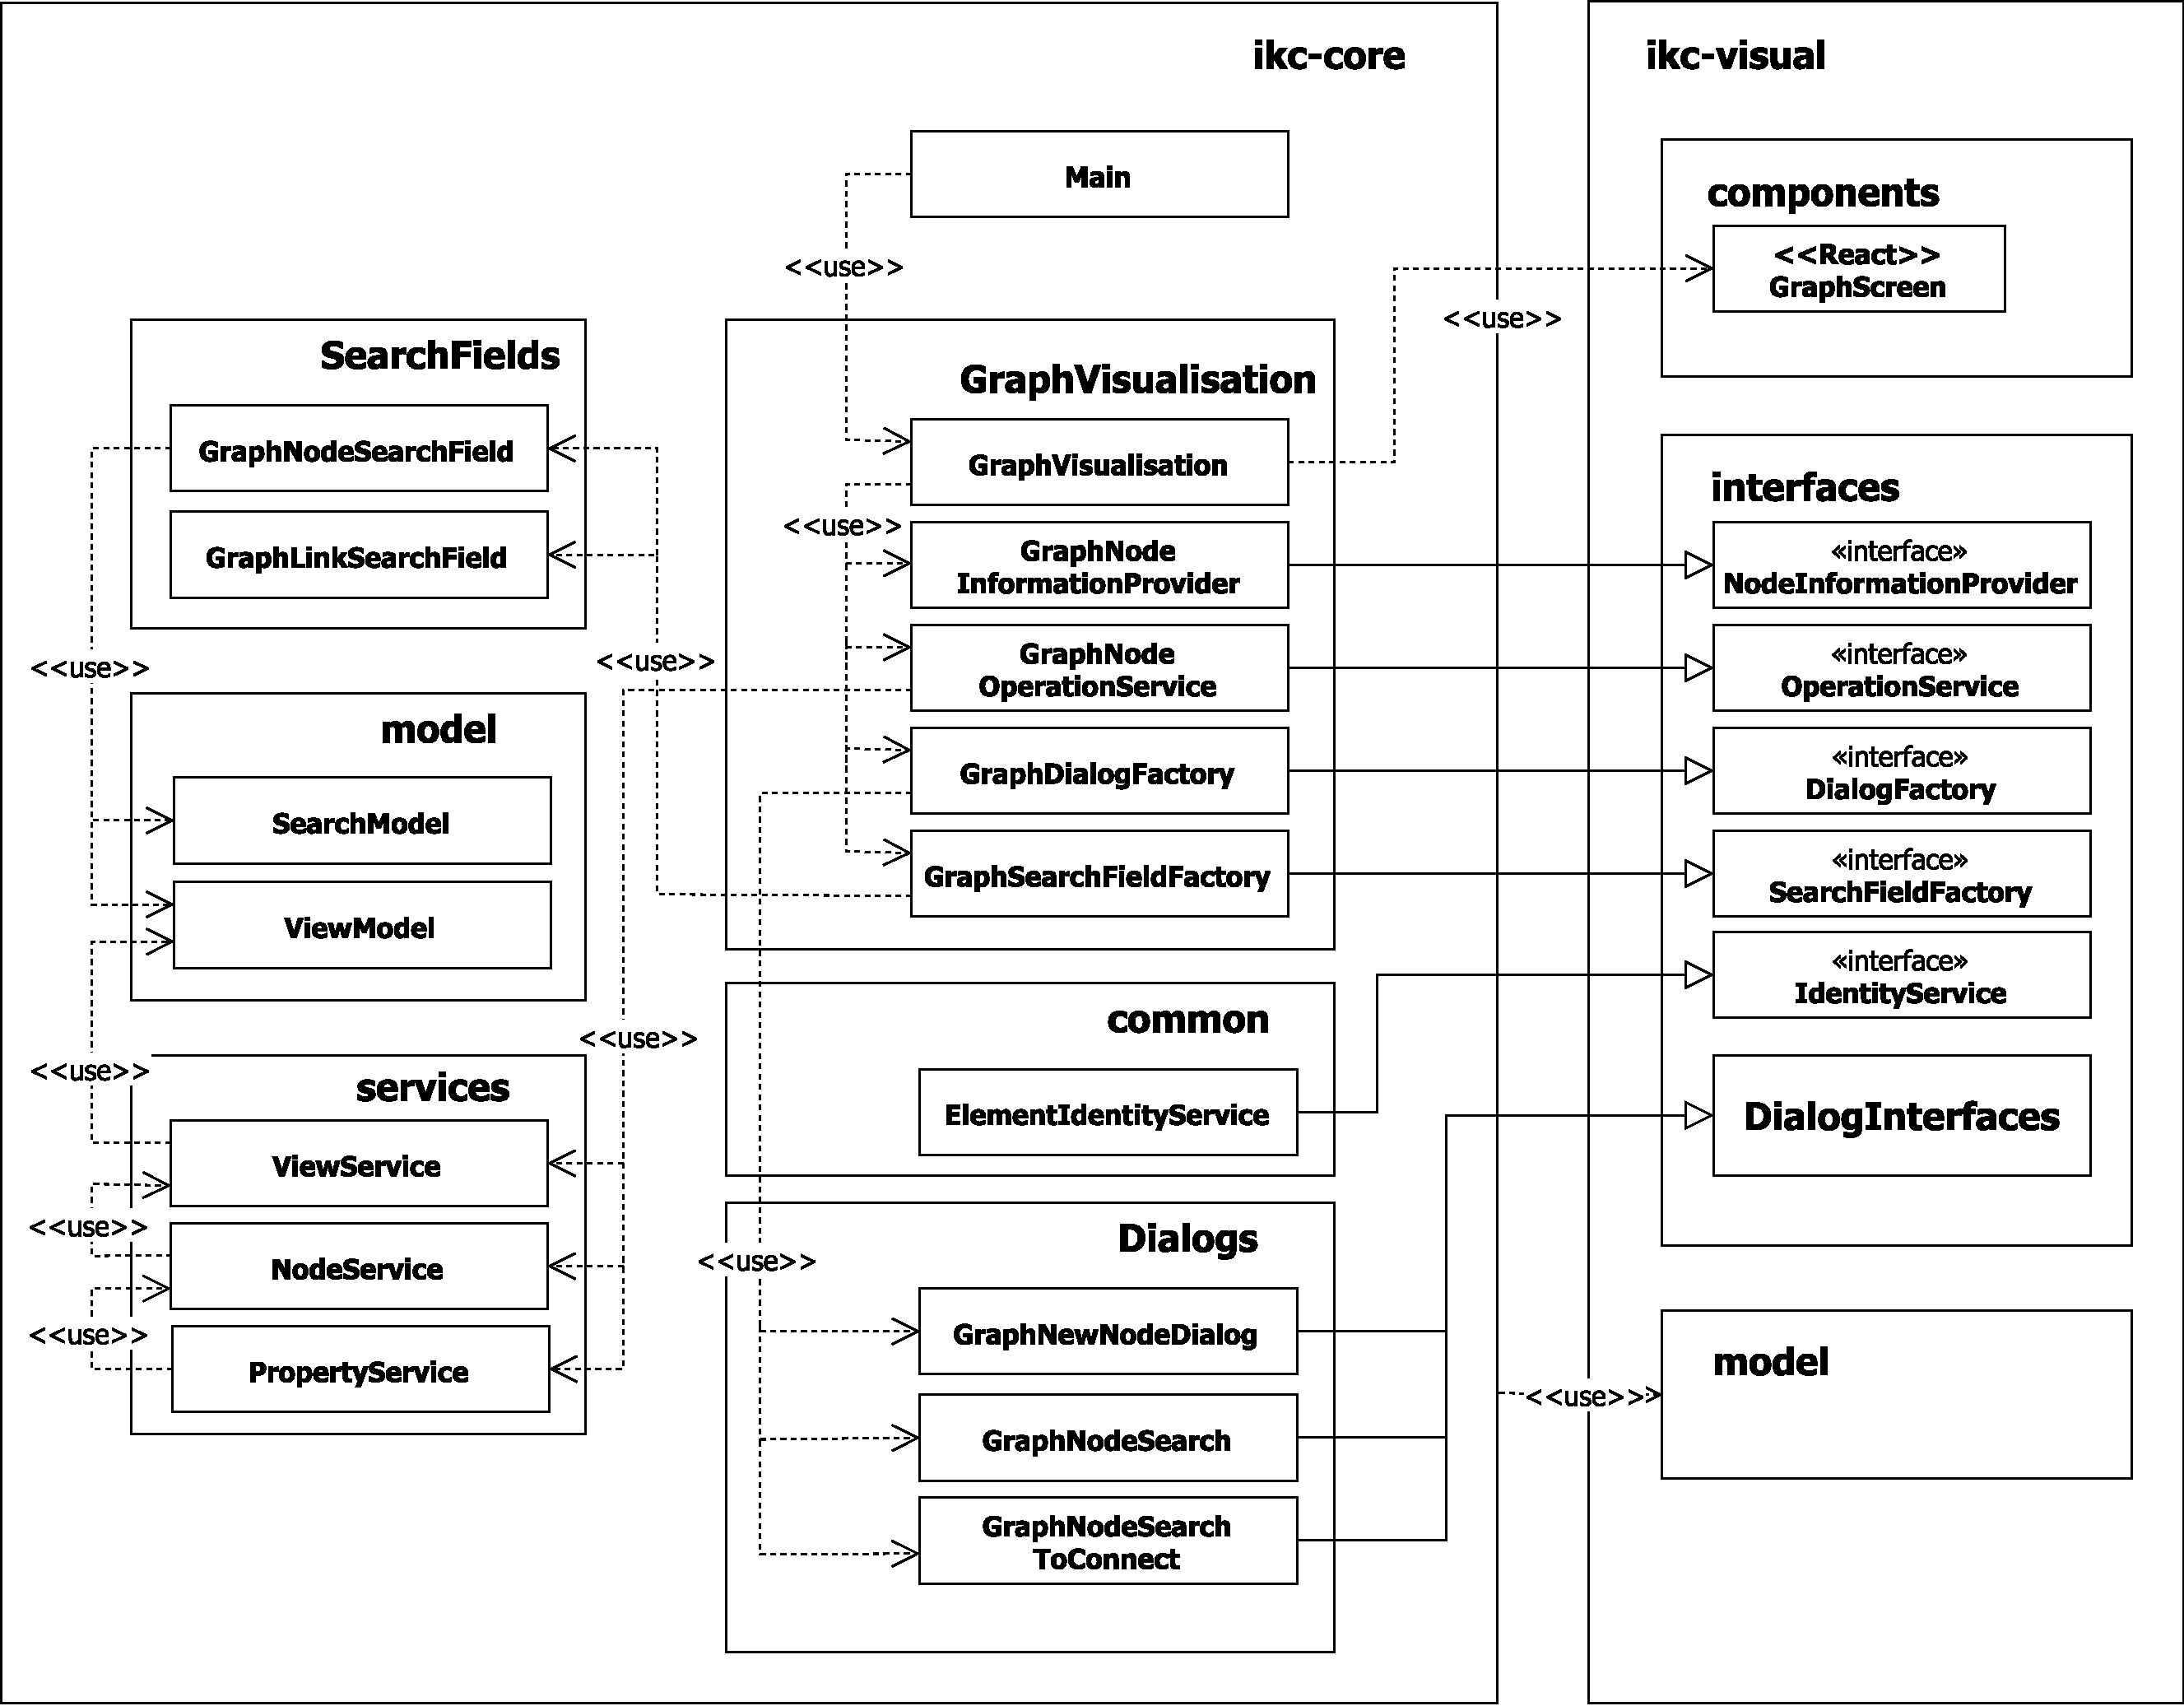
\includegraphics[width=1.3\textwidth]{ikc-visual-integration}}
\caption{Intergration Visualisierung}
\label{fig:integration-visualisation}
\end{figure}



\chapter{Schlussfolgerungen}
Mit dem Abschluss dieser Arbeit wird ein Prototyp einer Visualisierung zur intuitiven Interaktion mit einem Wissensnetzwerk präsentiert. Dieser Prototyp wurde losgelöst von der Hauptapplikation (\gls{ikc-core}) entwickelt und kann als externes Software-Packet verwendet werden. Durch das Erfüllen aller Testfälle des Testkonzepts sind sämtliche Anforderungen erfüllt.

Der Prototyp ermöglicht dem Benutzer ein besseres Verständnis und einfacheren Zugang zur Datenbasis des \gls{ikc-core}[s]. Zusätzlich wurde der Funktionsumfang erweitert: Mittels den neu eingeführten \gls{View}[s] kann ein \gls{Netzwerk} weiter unterteilt oder gar kontextuell gestaltet und dargestellt.
%Durch diesen Prototyp ist es nun möglich die zugrundeliegende Datenbasis des \gls{ikc-core} für den Benutzer besser zugänglich zu machen. Weiter kann der Benutzer mittels verschiedener Views, seine Wissensnetzwerk unterteilen und situationsangepasst darstellen. 

\section{Erkenntnisse}
Während der Durchführung dieser Arbeit haben wir uns vertieft mit der Visualisierung von \gls{Netzwerk}[en] und deren Interaktion beschäftigt. Dabei haben wir folgenden Erkenntnisse gewonnen: 

\begin{itemize}
    \item Durch die Evaluationen der verschiedenen \gls{Framework}s zu Beginn der Arbeiten verschafften wir uns einen breiten Überblick über bestehenden Lösungen. Zum einen konnten wir ein \gls{Framework} auswählen, welches unseren Anforderungen bestmöglich entspricht. Zum anderen erlangten wir dadurch einen Einblick in verschiedene Implementierungen und deren Konzept der Problemlösung
    %, im Bereich einer Netz\-werk-Vi\-su\-a\-li\-si\-er\-ung.
    Dadurch erhielten wir bereits vor der tatsächlichen Implementation ein gutes Gespür für die Thematik und deren Umsetzung, was schlussendlich zu einer guten Ressourcenplanung und Aufwandsschätzung führte. 
    \item Das \hyperref[cytoscape]{cytoscape}-\gls{Framework} überzeugt uns für die Visualisierung von \gls{Netzwerk}[en]: Es bietet eine Vielzahl von Erweiterungen, welche zusätzliche Funktionalität zur Verfügung stellen. Diese sind eigentlich für die Visualisierung von \gls{Netzwerk}[en] aus der Biologie %(zum Beispiel die Auswirkungen der Existenz von verschiedenen Genen) 
    gedacht. Welches nicht unserem Anwendungsfall entspricht. Trotzdem konnten wir verschiedene Konzepte davon aufgreifen und somit unsere Lösung zu modellieren. 
    \item Die Darstellung von \gls{Netzwerk}[en] und deren Interaktion wird schnell unübersichtlich. Insbesondere, falls \gls{Link}[s] in beide Richtungen existieren oder dadurch Schleifen über mehrere Ebenen entstehen.
    \item Auch die Interaktion mit einem \gls{Netzwerk} gestaltet sich schwieriger als erwartet. Beispielsweise erweist sich das Zuklappen von \gls{Link}[s] als ein Vorgang mit diversen Abhängigkeiten: Gibt es mehrere \gls{Link}[s] an einem \gls{Node}, wird anders reagiert als wenn nur ein \gls{Link} oder keiner existiert. Somit können gleiche Aktionen je nach \gls{Netzwerk}-Kontext unterschiedliche Resultate ergeben.
    \item Die Verwendung auf mobilen Geräten mit kleinem Bildschirmen erfordert besondere Beachtung. Dabei müssen Aktionen für den Benutzer möglichst einfach erreichbar sein und gleichzeitig darf die Applikation nicht überladen wirken. Die Bedienung mit den Fingern hat andere Anforderungen als eine Bedienung mit der Maus und Tastatur.
    \item Die Interaktion mit einer Benutzeroberfläche kann bereits vor der Implementierung konzeptionell genau geplant werden. Die Missachtung von kleinen Details kann unter Umständen später zu Unklarheiten und erheblichem Zusatzaufwand führen.
    %Definitionen von der Benutzung einer Applikation sind essentiell für die nachfolgende Implementierung. Dabei verursachen die Missachtung von kleinen Details in der Konzeption oft grosse Unklarheiten, welche mit einer exakten Definition verhindert werden kann.    
\end{itemize}

\section{Lessons learned}
Basierend auf den Erkenntnissen und der Reflexion unserer Arbeit, sind die folgenden Punkte, die wichtigsten Schlüsse, welche wir aus dem Modul mitnehmen:
\begin{itemize}
    \item Die Anforderungen an die Benutzeroberfläche und deren Bedienung müssen möglichst früh genau festgelegt werden. Obwohl wir dies zum Teil gemacht haben, tauchten im Laufe der Entwicklung diverse Unklarheiten auf. Mit detaillierteren Anforderungen und genaueren Modellen, hätten diese vermieden werden können.
    %hätten wir, mit einem höheren Detailgrad, Unklarheiten in der Implementierung vermeiden können.
    \item Durch das punktuelle Ein- und Ausblenden der Beschriftungen von \gls{Link}[s] kann die Übersichtlichkeit in grossen Netzwerken zusätzlich erhöht werden. 
    %Da die Übersichtlichkeit mit der Grösse des \gls{Netzwerk}[s] stark abnimmt, kann durch das punktuelle Ein- und Ausblenden der \gls{Link}-Labels diese erhöht werden.
    \item Die vom \gls{ikc-core} losgelöste Entwicklung erzwang eine komplett eigenständige Entwicklung gleich von Beginn an. Dadurch war eine lose Kopplung und gleichzeitige hohe Kohäsion stets gewährleistet.
    %Durch die Entwicklung des Prototypen, losgelöst vom gls{ikc-core}, waren wir gezwungen die Archtektur und unsere Arbeitsweise einer möglichst geringen Kopplung und einer starker Kohäsion zu unterstellen. 
    \item Aufgrund der internationalen Projektorganisation musste den Methoden und den Mittel für eine Kollaboration besondere Beachtung geschenkt werden. Mit den angegebenen Hilfsmitteln funktionierte dies ausgezeichnet. Trotz den gegebenen Um\-ständ\-en war eine enge Zusammenarbeit und ein ständiger Austausch stets gegeben. Sehr hilfreich waren dabei auch Bildschirmaufzeichnungen. Die grösste Herausforderung stellte sicherlich die zeitlichen Koordinaten dar. Besprechungen wurden darum mög\-lich\-st regelmässig zu fixen Zeiten abgehalten.
    
    Die Auslastung konnte stets gut der aktuellen Situation angepasst werden. So konnten sich Andreas Waldis im Dezember und Patrick Siegfried im Januar praktisch ausschliesslich den Prüfungen widmen. Auch konnte an Teile der Arbeit gut unabhängig gearbeitet werden, sodass der Arbeits-Fortschritt trotz zeitweiser intensiver Auslastung nie ausblieb. Eine Erleichterung war die Erweiterung des Zeitrahmens seitens der HSLU. Dadurch war es einfacher möglich die Arbeit trotz den unterschiedlichen Semesterterminen erfolgreich abzuschliessen.
    %Durch die Zusammenarbeit zwischen Amerika und der Schweiz über weite Dauer der Arbeit, musste einen besonderen Stellenwert auf Methoden und Mittel der Zusammenarbeit gelegt werden. Dies funktionierte vor allem durch die Verwendung der verschiedenen Hilfsmittel sehr gut. Hilfreich war insbesondere die enge Zusammenarbeit und der Austausch ausserhalb dieser Arbeit. So bestand ein ständiger Informationsfluss welcher nicht mit grossem Aufwand aufrechterhalten werden musste. Die grösste Herausforderung war dabei die zeitliche Koordination von Besprechungen und Ressourcenplanung. So wurden fix Termine in einen zeitlich normierten Kalender eingetragen und Auslastung entsprechend der aktuellen Situation angepasst. So konnte sich Andreas Waldis im Dezember auf seine Abschlussprüfungen konzentrieren und Patrick Siegfried betrieb einen grösseren Aufwand. Nach der Rückkehr von Amerika konnte dann die Situation umgekehrt werden, da Patrick Siegfried im Januar mit seinen Prüfungen beschäftigt war. Ebenfalls war es eine grosse Hilfe, dass der Zeitraum der Arbeit um einen Monat von der HSLU erweitert wurde. 
\end{itemize}

\section{Ausblick}
Der präsentierte Prototyp erfüllt die Anforderungen und ist in den \gls{ikc-core} integriert. Jedoch gibt es verschiedene mögliche Optimierungen:
\begin{itemize}
    \item Mit Hilfe der Erweiterung \textit{cytoscape.js-undo-redo} können Operationen rückgängig gemacht werden. Dies könnte zum Beispiel eine nutzliche Funktion sein, um versehentlich gelöschte Elemente wiederherzustellen. \citep{cytoscape-js-undo-redo}.
    \item Beim Hinzufügen eines neuen \gls{Node}[s] wird dieser automatisch zufällig unter dem Eltern-\gls{Node} angezeigt. Dies kann problematisch werden, falls exakt an dieser Stelle bereits ein \gls{Node} angezeigt wird. Dies könnte verhindert werden, indem die Positionen aller bereits angezeigten Nodes berücksichtigt würde.
    %Aktuell wird die Position eines \gls{Node}[s] zufällig unter dem Eltern \gls{Node} berechnet. So kann es sein das dieser Stelle bereits ein anderer \gls{Node} oder \gls{Link} dargestellt wird. Dies könnte verhindert werden mit der Berücksichtigung aller bereits dargestellten \gls{Node}[s] in der Positionsberechnung. 
    \item Durch die Verwendung von verschiedenen Farben, Formen und Grössen wäre es möglich \gls{Node}[s] unterschiedlicher grafisch zu differenzieren, und so unterschiedliche \gls{Node}-Typen sichtbar hervorzuheben. Die Erweiterung \textit{cytoscape.js-supportimages} würde eine Einbindung von Piktogrammen ermöglichen. \citep{cytoscape-js-supportimages}.
    \item Die Erweiterung \textit{js-cytoscape-navigator} zeigt eine Übersicht über das dargestellte Netzwerk an. Der Vorteil ist vor allem die erhöhte Übersicht in grossen \gls{Netzwerk}[en].
    %Mit einer kleine Übersicht über dem dargestellten Netzwerk, würde die Übersicht auf kleinen Monitoren zunehmen. Dies wird durch die Erweiterung \textit{js.cytoscape-navigator} angeboten \citepp{js.cytoscape-navigator}. 
    \item Die Erweiterung \textit{cytoscape.js-clipboard} bietet 'Copy-Paste'-Funk\-tio\-na\-li\-tät. Damit könnten Teile einer \gls{View} wiederverwendet werden. \citep{cytoscape-js-clipboard}.
    \item Eine denkbare Erweiterung ist eine automatische Generierung von \gls{View}[s]. Diese würde dem Benutzer eine Übersicht über sein Wissen bieten. Es ist vorstellbar, dass er bestimmte Parameter, beispielsweise die Tiefe des darzustellenden Netzwerks von einem gewählten Ausganspunkt aus, beeinflussen kann. 
    %Mit Hilfe von automatischer Generierung von Visualisierung könnte einem Benutzer einfach eine Übersicht über die Umgebung eines \gls{Node}[s] gewährt werden. So ist es Vorstellbar, bei Bedarf eine \gls{View} zu generieren, welche einen ausgewählten \gls{Node} und alle \gls{Node}[s] welche über n-Ebenen verbunden sind.
    \item \hyperref[cytoscape]{cytoscape} hat seine Ursprünge in der \gls{Netzwerk}-Theorie. Darum bietet es neben der Darstellung auch diverse Algorithmen an. Dazu gehören beispielsweise bekannte Algorithmen \textit{Dijkstra} oder auch \textit{A*}. \citep{cytoscape-js}
    %\hyperref[cytoscape]{cytoscape} bietet neben der ganzen Visualisierung auch eine Struktur um \gls{Node}[s] und \gls{Link}[s] strukturiert zu halten und entsprechende Operation. Dazu gehören verschieden Algorithmen welche für Graphen und Netzwerken bekannt sind. So zum Beispiel \textit{Dijkstra} oder \textit{A*} \citep{cytoscape.js}.
    \item Ab einer gewissen \gls{Node}-Titellänge wird die Darstellung un\-gün\-stig. Der Titel ragt über die jeweilige Komponente. Dies könnte einfach mit \gls{CSS} oder \gls{Javascript} gelöst werden.
\end{itemize}

\bibliographystyle{apacite}
\bibliography{refs}

\renewcommand\listoflistingscaption{Code}
\listoflistings

%\appendix

%\chapter{Dummy Appendix}

You can defer lengthy calculations that would otherwise only interrupt
the flow of your thesis to an appendix.


\backmatter

\end{document}
